\documentclass{article}

% Language setting
\usepackage[T1,T2A]{fontenc}
\usepackage[utf8]{inputenc}
\usepackage[english,russian]{babel}

% Set page size and margins
\usepackage[letterpaper,top=2cm,bottom=2cm,left=3cm,right=3cm,marginparwidth=1.75cm]{geometry}

% Useful packages
\usepackage{amsmath}
\usepackage{graphicx}
\usepackage[colorlinks=true, allcolors=blue, unicode, pdftex]{hyperref}
\usepackage{diagbox}
\usepackage{caption}
\captionsetup[table]{justification=centering}
\usepackage{blindtext}
\usepackage{titlesec}
\usepackage{indentfirst}
\addto\captionsrussian{\def\refname{Список используемой литературы}}
\usepackage{subfigure}
\usepackage[toc,page]{appendix}
\usepackage{float}
\usepackage{tikz}
\usepackage{amssymb}

\begin{document}

\begin{titlepage}
\begin{center}
    Московский государственный университет имени М. В. Ломоносова

    \bigskip
    
\includegraphics[width=70mm]{msu.eps}

    \bigskip
    Факультет Вычислительной Математики и Кибернетики\\
    Кафедра Математических Методов Прогнозирования\\[10mm]
    
    \textsf{\large\bfseries
        Отчет по второму заданию курса "Практикум на ЭВМ"\\[10mm]
        "Градиентные методы обучения линейных моделей"
    }\\[10mm]
    \begin{flushright}
        \parbox{0.5\textwidth}{
        	Выполнила:\\
        	студентка 3 курса 317 группы \\
        	\emph{Кривуля Полина Юрьевна}\\[5mm]
        }
    \end{flushright}
    \vspace{\fill}
    Москва, 2022
\end{center}
\end{titlepage}

\newpage
\tableofcontents
\newpage

\section{Введение}
Градиентный спуск относится к оптимизационным алгоритмам и используется для настройки параметров модели машинного обучения.

При стандартном (или «пакетном», «batch») градиентном спуске для корректировки параметров модели используется градиент. Градиент обычно считается как сумма градиентов, вызванных каждым элементом обучения. Вектор параметров изменяется в направлении антиградиента с заданным шагом. Поэтому стандартному градиентному спуску требуется один проход по обучающим данным до того, как он сможет менять параметры.

При стохастическом (или «оперативном») градиентном спуске значение градиента аппроксимируется градиентом функции стоимости, вычисленном только на одном элементе обучения. Затем параметры изменяются пропорционально приближенному градиенту. Таким образом параметры модели изменяются после каждого объекта обучения. Для больших массивов данных стохастический градиентный спуск может дать значительное преимущество в скорости по сравнению со стандартным градиентным спуском.

Между этими двумя видами градиентного спуска существует компромисс, называемый иногда «mini-batch». В этом случае градиент аппроксимируется суммой для небольшого количества обучающих образцов \cite{ss0}.

В данном исследовании изучается работа градиентного спуска и стохастического градиентного спуска для различных параметров на примере задачи биномиальной классификации текстов для определения токсичности комментария.

\section{Теоретическая часть}
\subsection{Градиент функции потерь для задачи бинарной логистической регрессии}

Функция потерь для задачи бинарной логистической регрессии представима в виде:

$$Q(X, w) = \frac{1}{l}\sum_{i=1}^l\mathcal{L}(M_i(w))+\frac{\lambda}{2}\|\\w\|_2^2,$$

где $\mathcal{L} = \log{(1+exp(-M))},\: M = y_i\langle w, x_i\rangle$


Так как $d(1 + exp(-y_i\langle w, x_i\rangle)) = d(exp(-y_i\langle w, x_i\rangle)) = - exp(-y_i\langle w, x_i\rangle) * y_i\langle x_i, dw\rangle,$


$d(\|w\|_2^2) = \langle 2w, dw\rangle,$


$$dQ(X, w) = \frac{1}{l}\sum_{i=1}^l\frac{ - exp(-y_i\langle w, x_i\rangle) * y_i\langle x_i, dw\rangle}{1 + exp(-y_i\langle w, x_i\rangle)}  + \lambda \langle w, dw\rangle $$

$$\Rightarrow \triangledown_w Q(X, w) = \frac{1}{l}\sum_{i=1}^l\frac{ - exp(-y_i\langle w, x_i\rangle) * y_i * x_i}{1 + exp(-y_i\langle w, x_i\rangle)}  + \lambda w $$



\subsection{Градиент функции потерь для задачи многоклассовой логистической регрессии}

Функция потерь для задачи мультиномиальной логистической регрессии (без регулязатора) представима в виде:

$$Q(X, w) = -\frac{1}{l}\sum_{i=1}^l\sum_{j=1}^K\left[y_i=j\right]log\frac{exp\langle w_i, x_i\rangle}{\sum_{z=1}^Kexp\langle w_z, x_i\rangle}$$

Найдем ее градиент для некоторого $w_q$:

$$\triangledown_{w_q}Q(w) = - \frac{1}{l}\sum_{i=1}^l\sum_{j=1}^K\left[y_i=j\right]\triangledown_{w_q}log\frac{exp\langle w_i, x_i\rangle}{\sum_{z=1}^K exp\langle w_z, x_i\rangle}$$

Так как $log\frac{exp\langle w_i, x_i\rangle}{\sum_{z=1}^Kexp\langle w_z, x_i\rangle} = log({exp\langle w_i, x_i\rangle}) - log(\sum_{z=1}^Kexp\langle w_z, x_i\rangle)$, 

$$\triangledown_{w_q}Q(w) = - \frac{1}{l}\sum_{i=1}^l\sum_{j=1}^K \left[y_i=j \right] ( x_i\left[ j = q\right] - \frac{x_i*exp\langle w_i, x_i\rangle}{\sum_{z=1}^K exp\langle w_z, x_i\rangle})$$


\subsection{Задача многоклассовой логистической регрессии при двух классах}

При двух классах задача многоклассовой логистической регрессии сводится к бинарной, при этом необходимо "переименовать"{ } классы на -1 и 1:

$$Q(X, w) = -\frac{1}{l}\sum_{i=1}^l\sum_{j=1}^2 \left[y_i=j\right]log\frac{exp\langle w_i, x_i\rangle}{\sum_{z=1}^2 exp\langle w_z, x_i\rangle} = $$

$$= -\frac{1}{l}\sum_{i=1}^l (\left[y_i=1\right]*log\frac{1}{1+exp\langle w_2 - w_1, x_i\rangle} + \left[y_i=2\right]*log\frac{1}{1+exp\langle w_1 - w_2, x_i\rangle}) = $$

$$=\frac{1}{l}\sum_{i=1}^l (\left[y_i=1\right]*log(1+exp\langle w_2 - w_1, x_i\rangle) + \left[y_i=2\right]*log(1+exp\langle w_1 - w_2, x_i\rangle)) = $$

Воспользуемся переходом $\left\{1, 2\right\} \rightarrow \left\{-1, 1\right\} $

$$= \frac{1}{l}\sum_{i=1}^l (\left[y_i=-1\right]*log(1+exp\langle w_{+1} - w_{-1}, x_i\rangle) + \left[y_i=+1\right]*log(1+exp\langle w_{-1} - w_{+1}, x_i\rangle)) =$$

$$=  \frac{1}{l}\sum_{i=1}^l log(1 + exp(-y_i*\langle w, x_i\rangle))$$

Функции потерь эквивалентны. Теперь докажем эквивалентность предсказаний моделей:
$$sign\langle w, x\rangle = (-1)* \left[ \langle w, x\rangle < 0\right] + (+1)* \left[ \langle w, x\rangle < 0\right] = {\underset{y\in\left\{-1, +1\right\}}{SoftMax}}\langle w_y, x\rangle = {\underset{y\in\left\{1, 2\right\}}{SoftMax}}\langle w_y, x\rangle$$


\subsection{Разностная проверка градиента}

Для проверки корректности аналитической формулы градиента функции потерь для задачи бинарной логистической регрессии реализован модуль численного подсчета, вычисляющий градиент приближенно по формуле:

$$\left[\triangledown f(w)\right]_i \approx\frac{f(x + \epsilon e_i) - f(x)}{\epsilon}$$

$e_i = (0, 0, 0, ..., 1, 0, ..., 0)$ – базисный вектор, $\epsilon > 0$ – небольшое положительное число.

На примере используемой в задании выборке при $\epsilon =10^{-8}$ квадрат нормы разности аналитического и численного подсчета вышел равным $1.4 * 10^{-12}$, что говорит о корректности аналитического расчета.


\section{Преобразование выборки}

В качестве предварительной обработки текста выполнены следующие действия:

\begin{itemize}
  \item Все тексты приведены к нижнему регистру;
  \item В тексте все символы, не являющиеся цифрами и буквами, заменены на пробелы, а много раз подряд встречающиеся пробелы заменены на один;
  \item Выборка преобразована в разреженную матрицу, где значение x в позиции (i,j) означает, что в документе i слово j встретилось x раз;
  \item Для уменьшения размерности признакового пространства и ускорения проведения экспериментов применен параметр min\_df=0.0001, уменьшивший размерность пространства с 89658 признаков до 16050.
\end{itemize}

Указанная обработка является стандартной и обычно позволяет улучшить качество работы алгоритма.
Выборка при этом представляется в виде «мешка слов» («Bag of words»). В этом представлении каждому тексту в соответствие ставится «мешок» его слов, в котором не учитывается расположение слов, а лишь их число вхождений в данный текст.


\section{Поведение используемых методов в зависимости от параметров}

Для минимизации функционала $Q(X, w)$  методом градиентного спуска выбирается начальное приближение для вектора весов $w$, затем запускается итерационный процесс, на каждом шаге которого вектор $w$ изменяется в направлении антиградиента функционала $Q(X, w)$:

$$w^{(k+1)}=w^{(k)}-\eta_k\triangledown_wQ(X,w), \:\:\:\:\:\:\: \hypertarget{formula}{(1)}$$

% ВОТ ССЫЛКА НА ФОРМУЛУ - (\hyperlink{formula}{1})

где $\eta_k=\frac{\alpha}{k^\beta}>0$ - темп обучения, монотонно уменьшающийся с течением итераций.

При этом во всех экспериментах выбрано значение регулязатора $\lambda=1$.

При стохастическом градиентном спуске градиент суммы оценивается градиентом подмножества слагаемых, на каждой итерации оно выбирается случайно. Это позволяет ускорить сходимость алгоритма.

В данном эксперименте проводится исследование поведения градиентного и стохастического градиентного спуска для задачи логистической регрессии при изменении следующих параметров:

\begin{itemize}
  \item Размера шага $\alpha$ (step\_alpha);
  \item Размера шага $\beta$ (step\_betta);
  \item Начального приближения весов.
\end{itemize}

Для стохастического градиентного спуска, помимо перечисленного, исследуется поведение метода при изменении размера подвыборки batch\_size.
Исследование поведения проводится при анализе зависимостей значения функции потерь и точности от итерации метода (эпохи в случае стохастического варианта). 



% альфа для граидиентного
\begin{figure}[H]
    \centering
    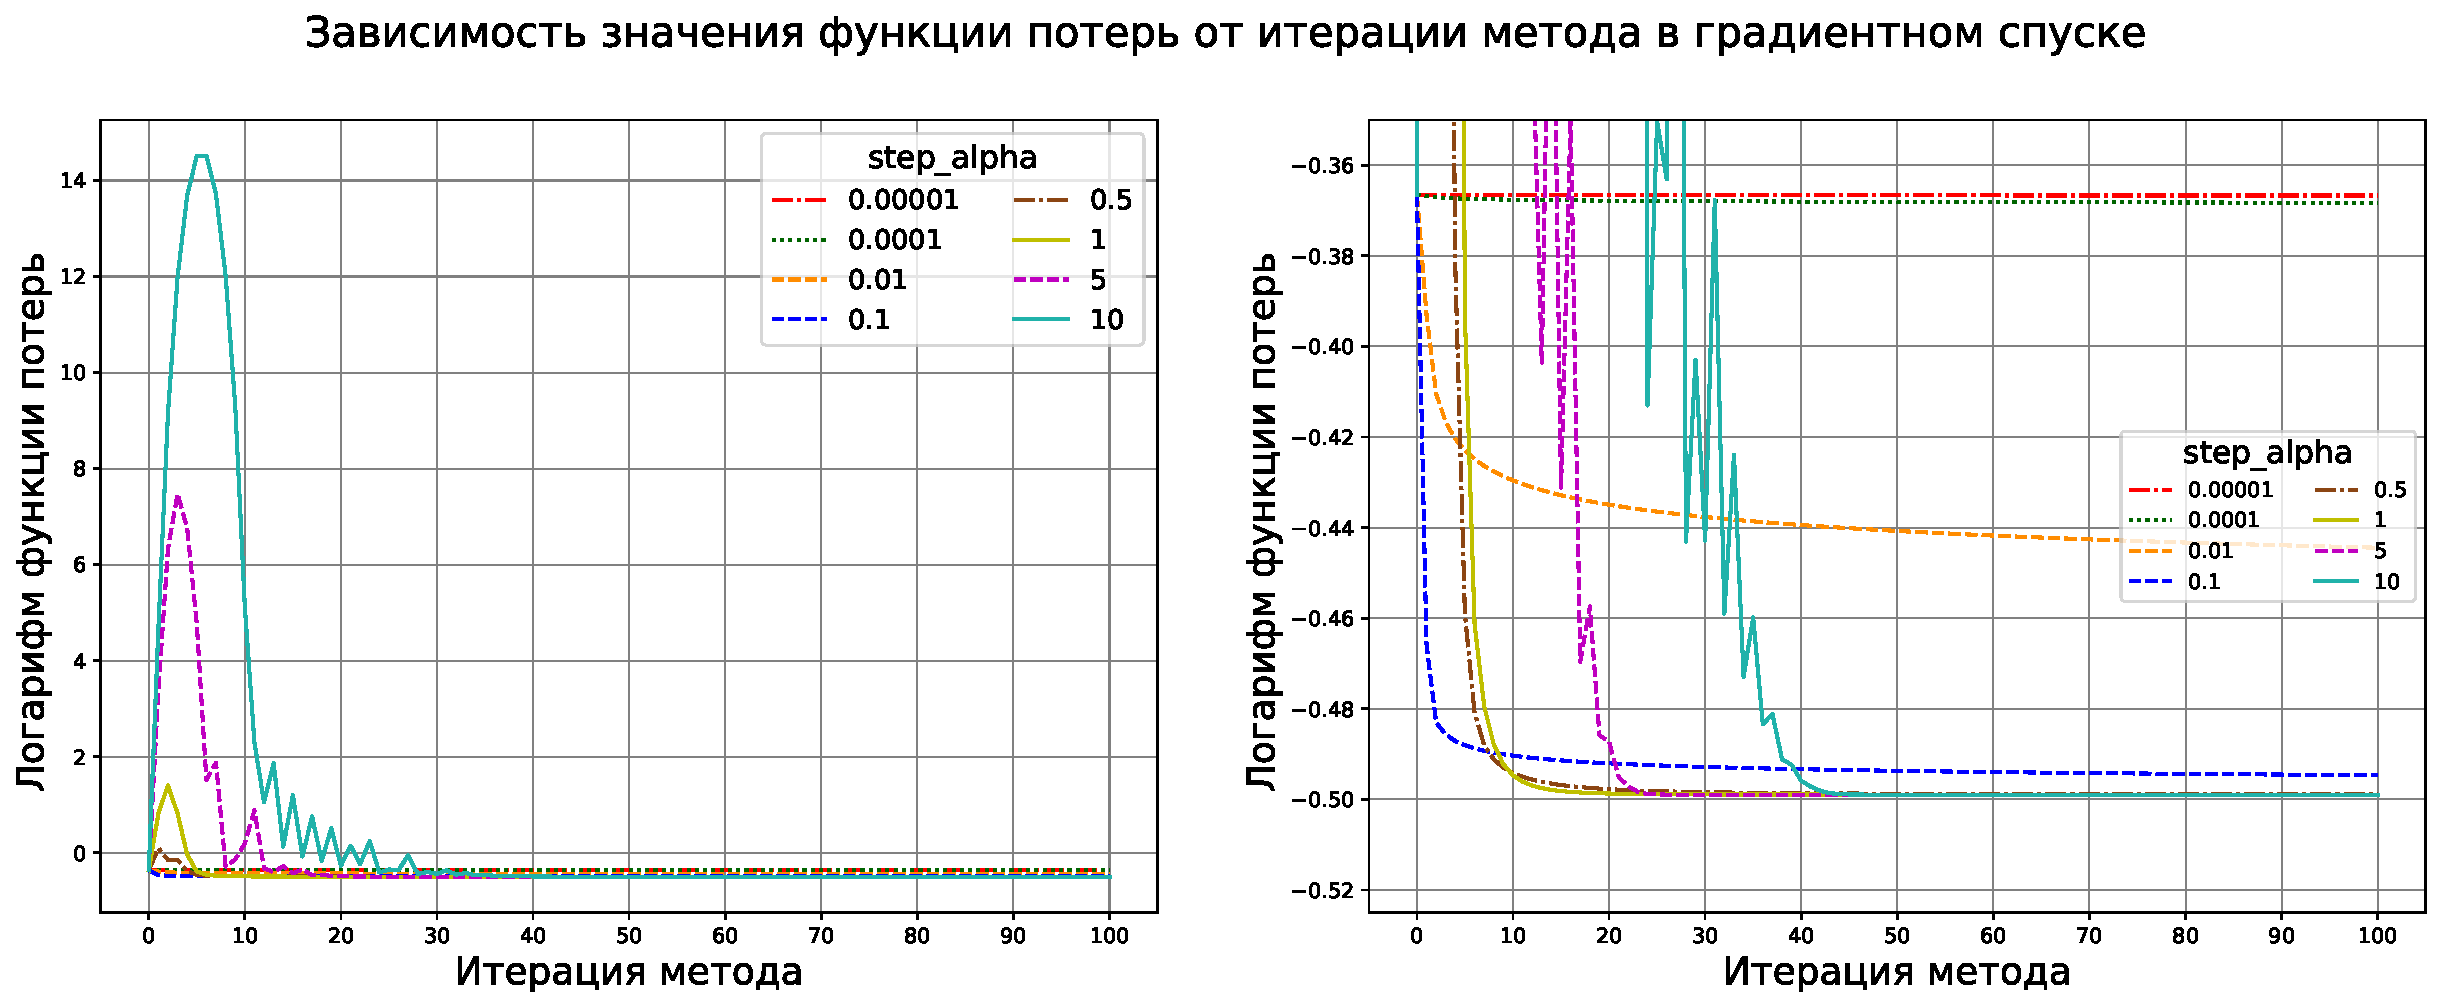
\includegraphics[width=15cm]{TASK2 step_alpha loss.pdf}
    \caption{Значения функции потерь в градиентном спуске при различных параметрах $\alpha$}
    \label{fig:step_alpfa_loss}
\end{figure}

\begin{itemize}
\item
Параметр $\alpha$ перебирается по сетке: \{0.00001, 0.0001, 0.01, 0.1, 0.5, 1, 5, 10\}. При исследовании данного параметра используется значение $\beta=1$ и нулевое начальное приближение весов, а для стохастического градиентного спуска batch\_size=10000. При значениях $\alpha > 1$ алгоритм становится менее устойчивым и медленнее сходится. При небольших значениях параметра алгоритм, напротив, слишком устойчив (градиентный спуск: рис. \ref{fig:step_alpfa_loss}, \ref{fig:step_alpfa_accuracy}, стохастический градиентный спуск: рис. \ref{fig:step_alpfa_loss_SGDC}, \ref{fig:step_alpfa_accuracy_SGDC}). Стохастический градиентный спуск при этом показывает результаты в среднем лучше.

\begin{figure}[H]
    \centering
    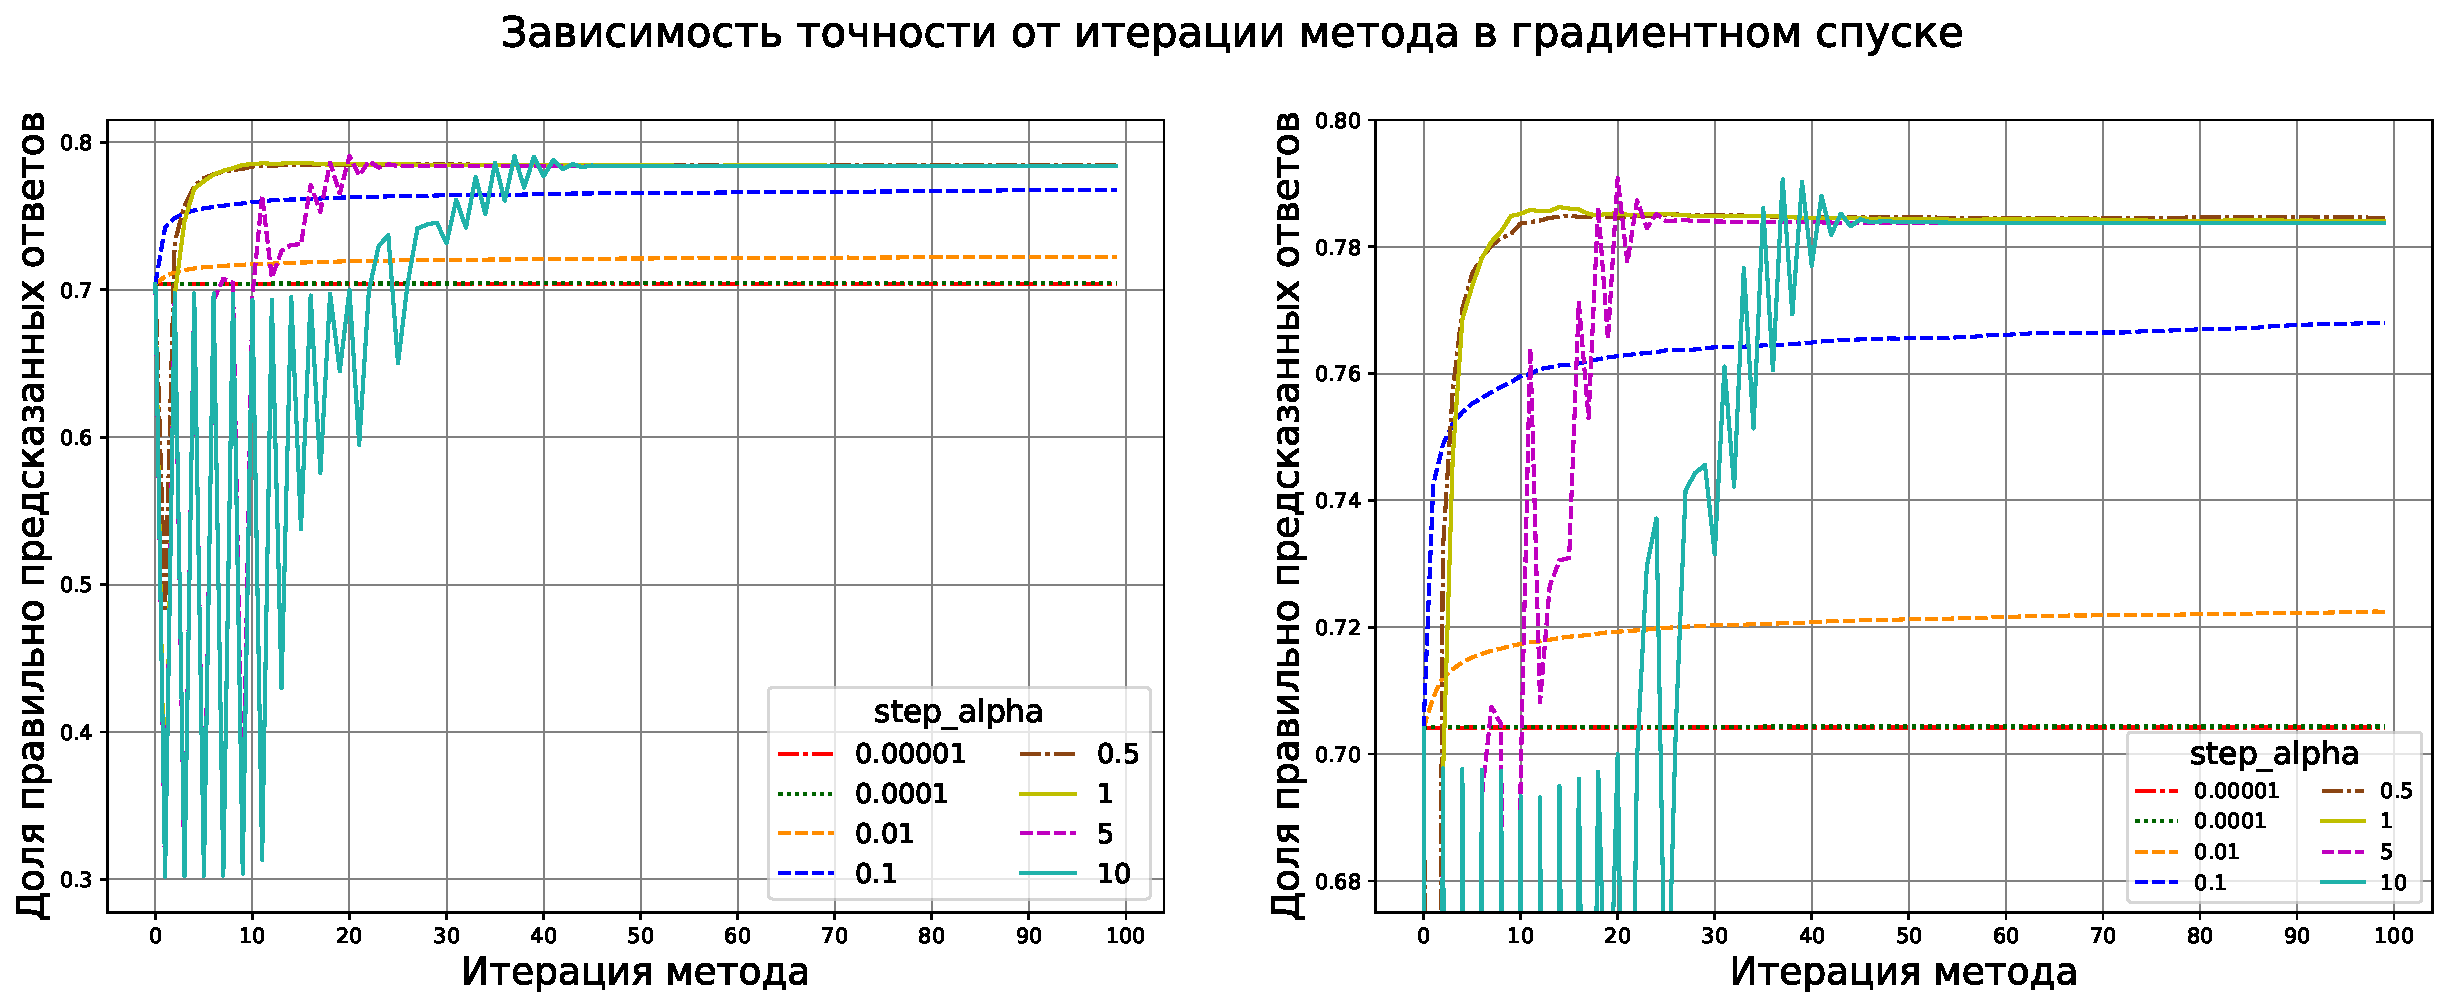
\includegraphics[width=14cm]{TASK2 step_alpha accuracy.pdf}
    \caption{Точность в градиентном спуске при различных параметрах $\alpha$}
    \label{fig:step_alpfa_accuracy}
\end{figure}


%альфа для стохастического
\begin{figure}[H]
    \centering
    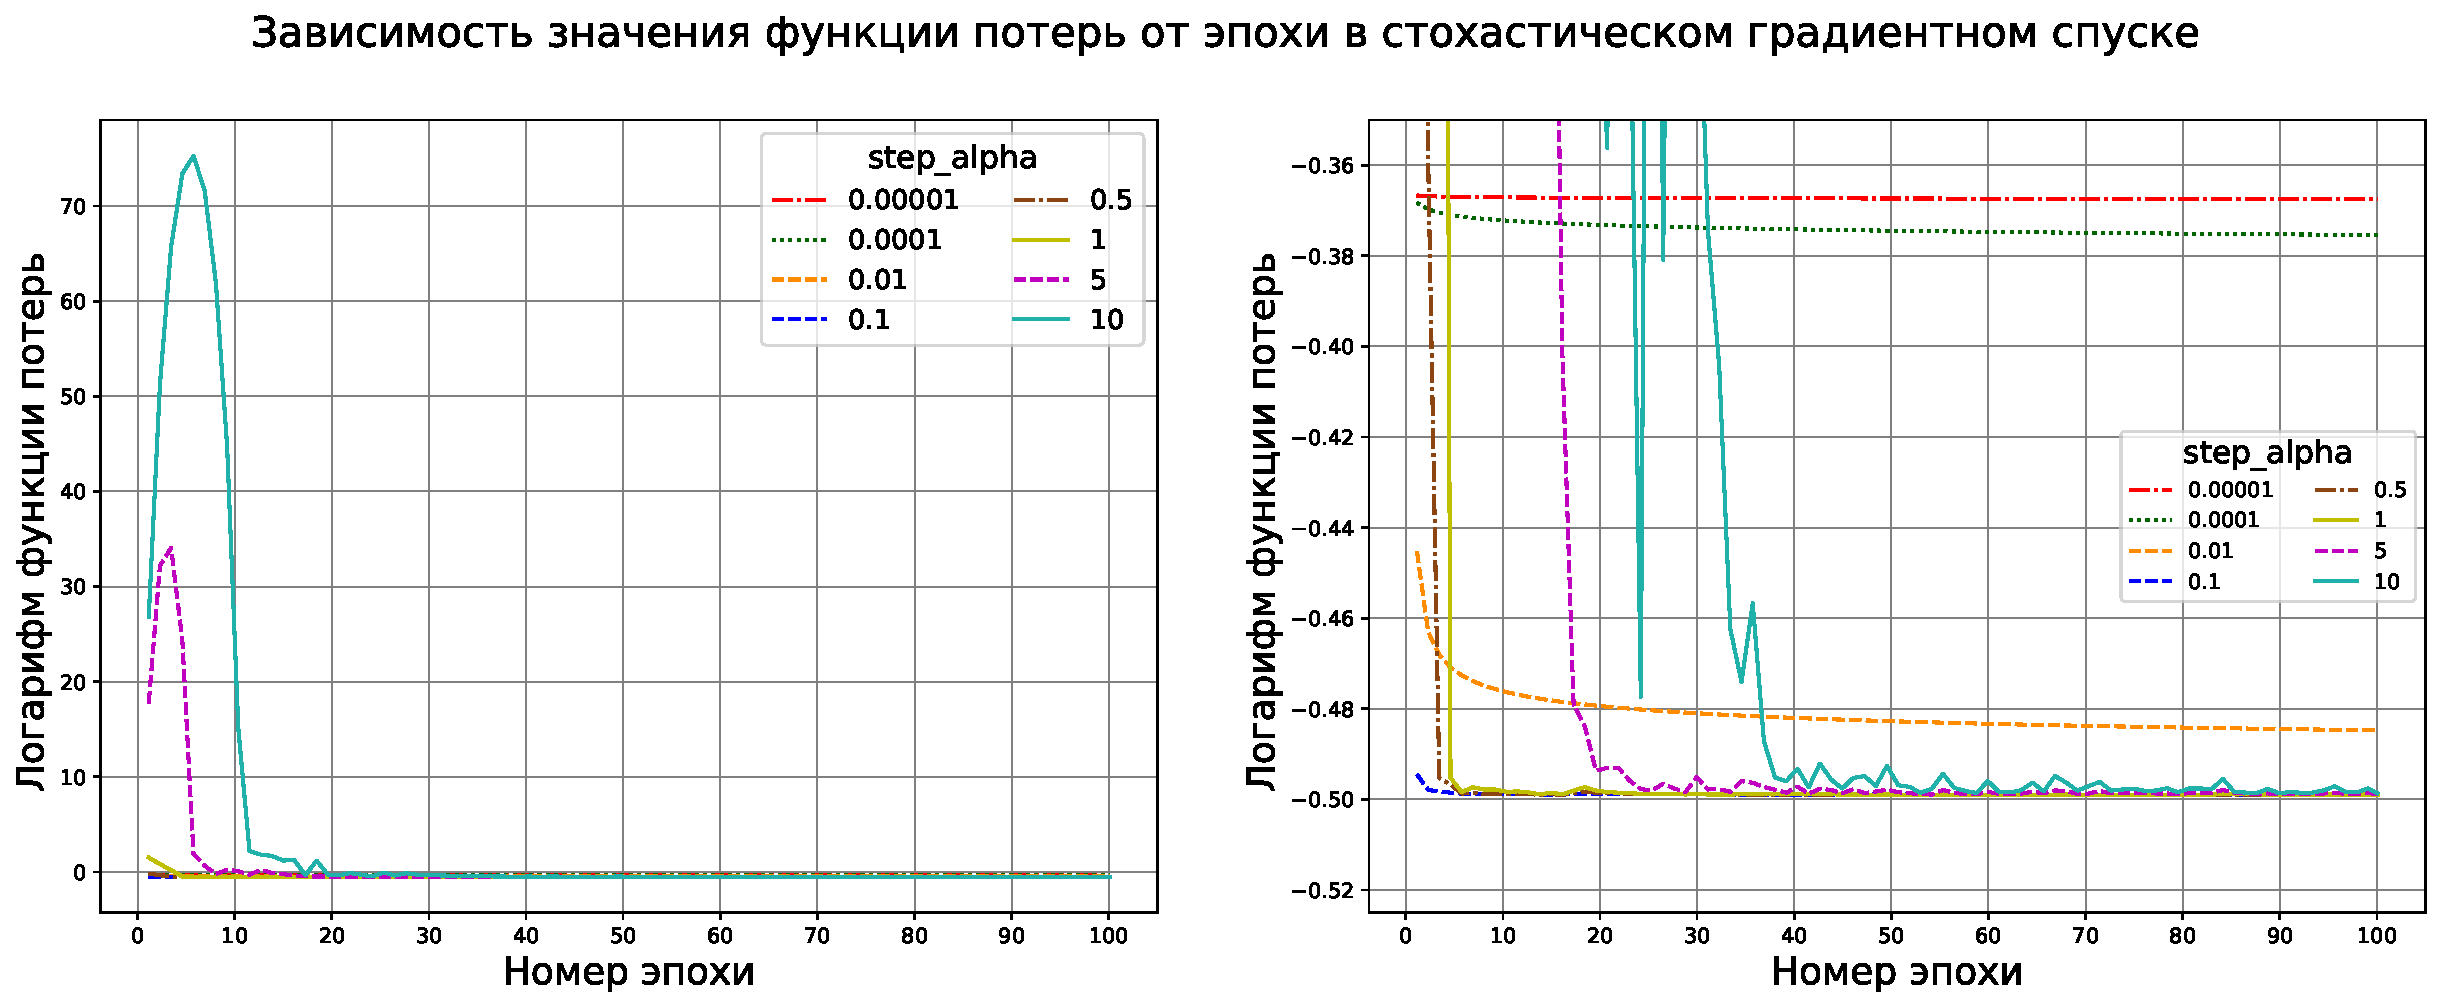
\includegraphics[width=14cm]{TASK2 step_alpha loss SGDClassifier.pdf}
    \caption{Функция потерь в стохастическом градиентном спуске при различных параметрах $\alpha$}
    \label{fig:step_alpfa_loss_SGDC}
\end{figure}
\begin{figure}[H]
    \centering
    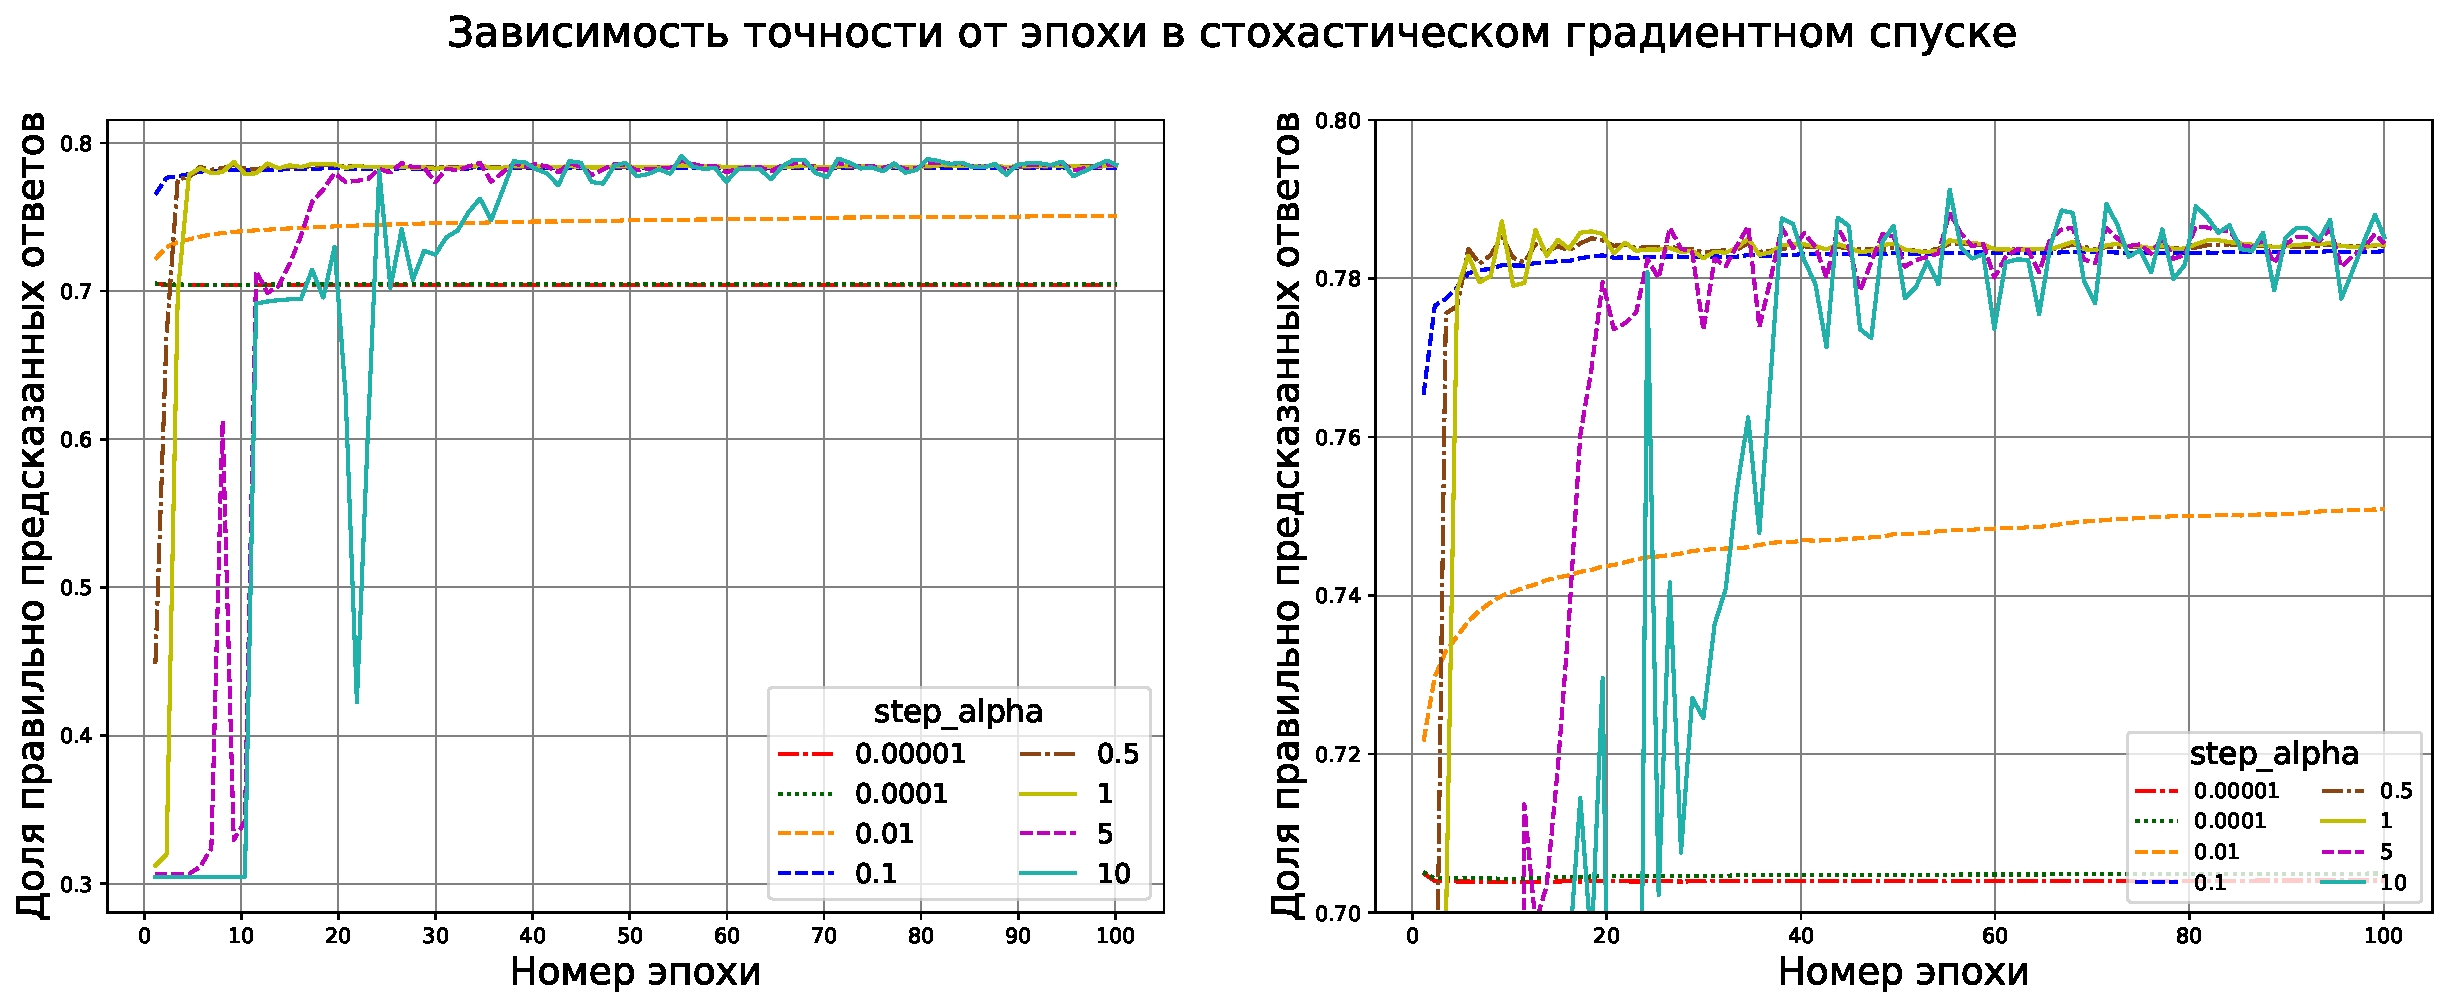
\includegraphics[width=14cm]{TASK2 step_alpha accuracy SDC.pdf}
    \caption{Точность в стохастическом градиентном спуске при различных параметрах $\alpha$}
    \label{fig:step_alpfa_accuracy_SGDC}
\end{figure}

\item
Параметр $\beta$ перебирается по сетке: \{0.1, 0.25, 0.5, 1, 1.01, 1.1, 5, 10, 100\}. При исследовании данного параметра используется значение $\alpha=0.5$ и нулевое начальное приближение весов, а для стохастического градиентного спуска batch\_size=10000. С уменьшением данного параметра алгоритм становится менее устойчивым, с увеличением, напротив, слишком устойчивым  (градиентный спуск: рис. \ref{fig:step_betta_loss}, \ref{fig:step_betta_accuracy}, стохастический градиентный спуск: \ref{fig:step_betta_loss_SGDC}, \ref{fig:step_betta_accuracy_SGDC}). При этом стохастический градиентный спуск показывает результаты в среднем лучше, и меньше колеблется при небольших значениях $\beta$. Однако, как и в случае с параметром $\alpha$, при "хороших"\ параметрах $\beta$, градиентный спуск ведет себя стабильно, в то время как стохастический градиентный спуск немного колеблется. Наиболее сильно это заметно на графиках точности (рис. \ref{fig:step_alpfa_accuracy} и  \ref{fig:step_alpfa_accuracy_SGDC}, рис. \ref{fig:step_betta_accuracy} и \ref{fig:step_betta_accuracy_SGDC}).

Влияние данных параметров ($\alpha$ и $\beta$) на устойчивость связано с формулой итерационного процесса (\hyperlink{formula}{1}). При увеличении $\alpha$ (уменьшении $\beta$) последующие значения весов сильнее начинают зависеть от значения градиента функционала, а при слишком малых $\alpha$ (больших $\beta$) значения градиента практически не меняют значения весов и алгоритм становится излишне устойчивым.

Далее используем значения $\alpha=0.5$ и $\beta=1.1$, если не оговорено обратного, так как они показали лучшие результаты в данном эксперименте.

% бета для градиентного
\begin{figure}[H]
    \centering
    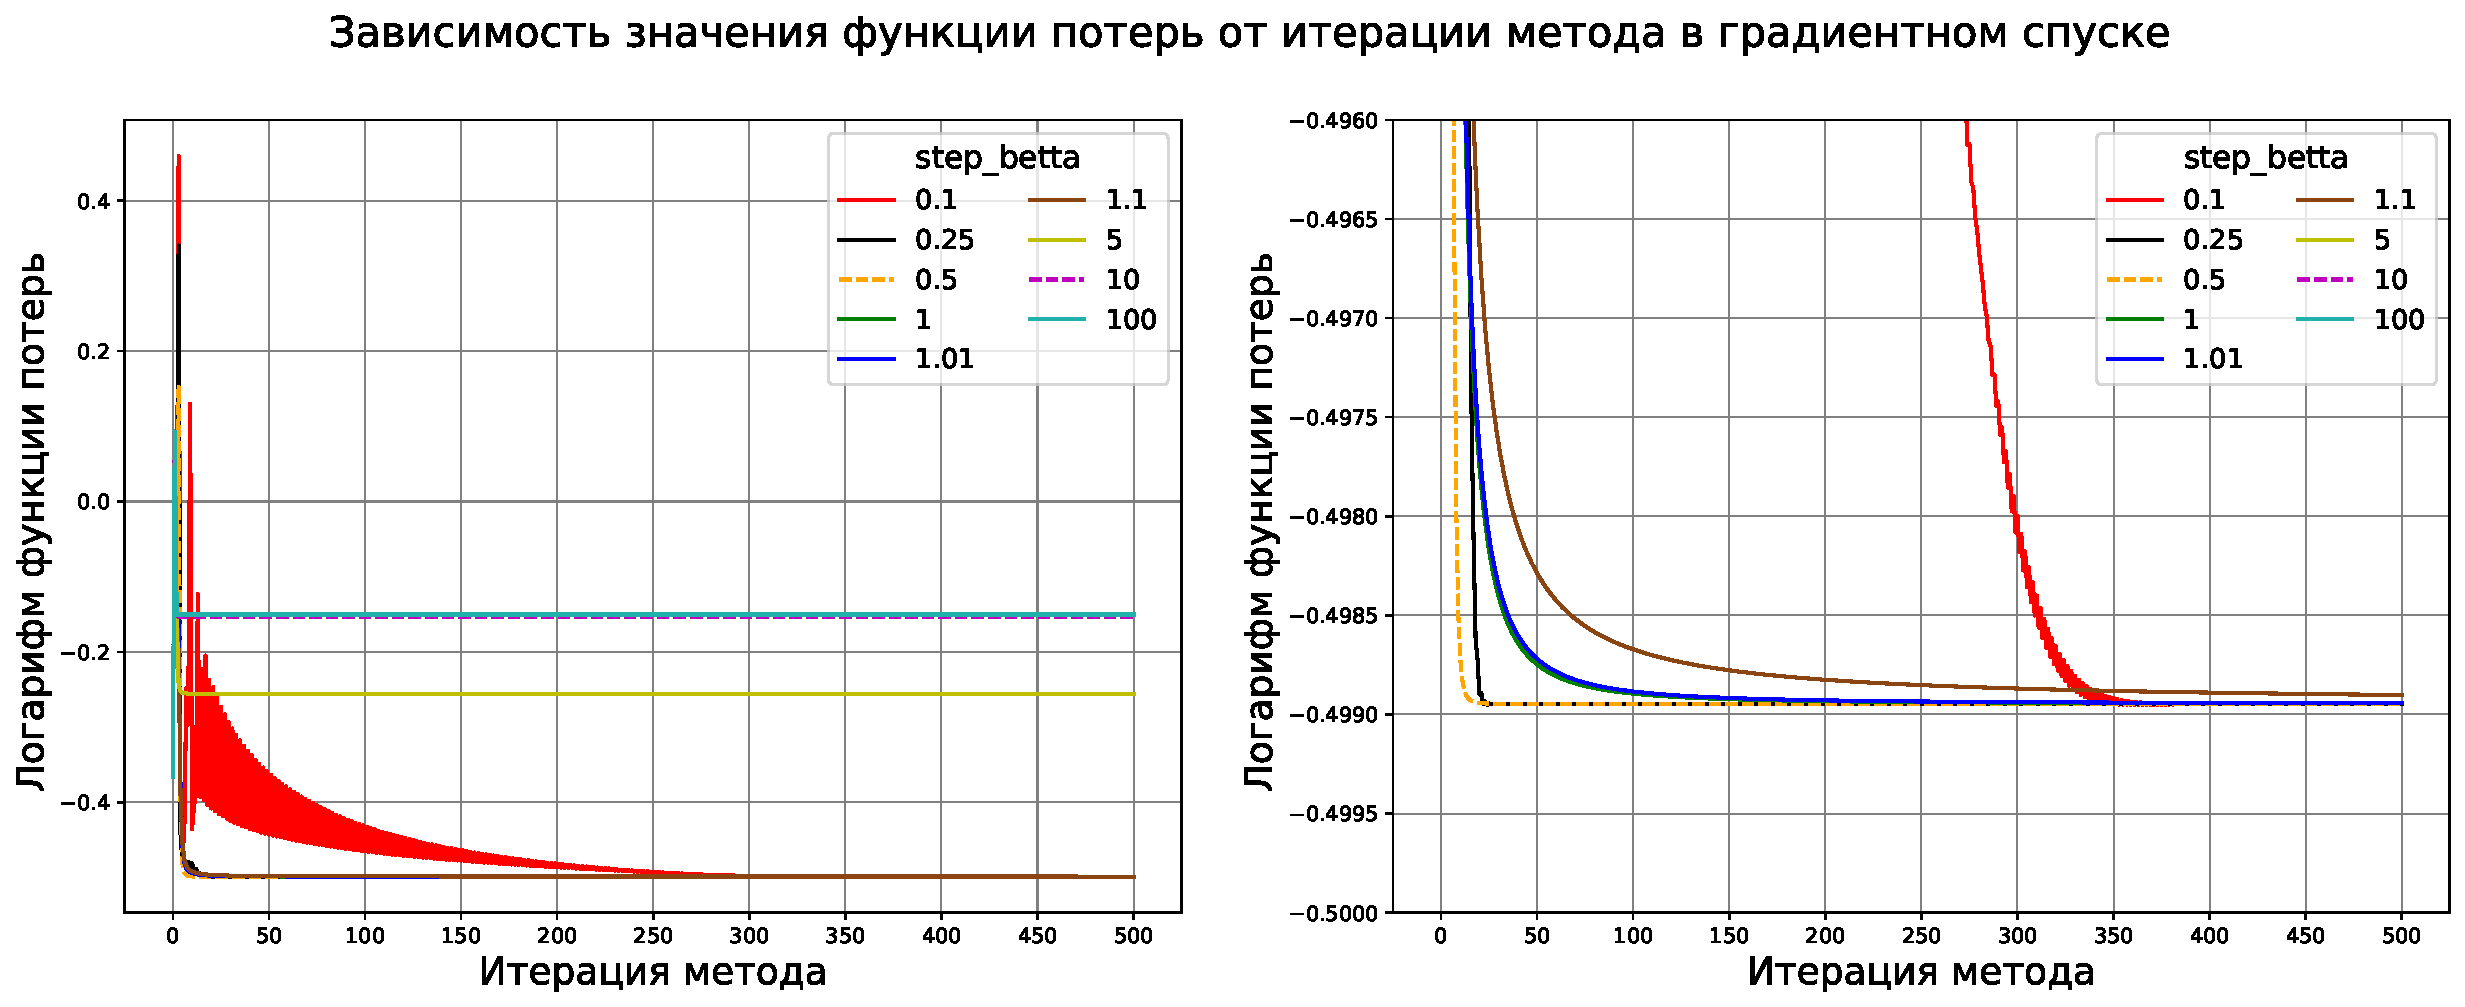
\includegraphics[width=15cm]{TASK2 step_betta loss.pdf}
    \caption{Значения функции потерь в градиентном спуске при различных параметрах $\beta$}
    \label{fig:step_betta_loss}
\end{figure}
\begin{figure}[H]
    \centering
    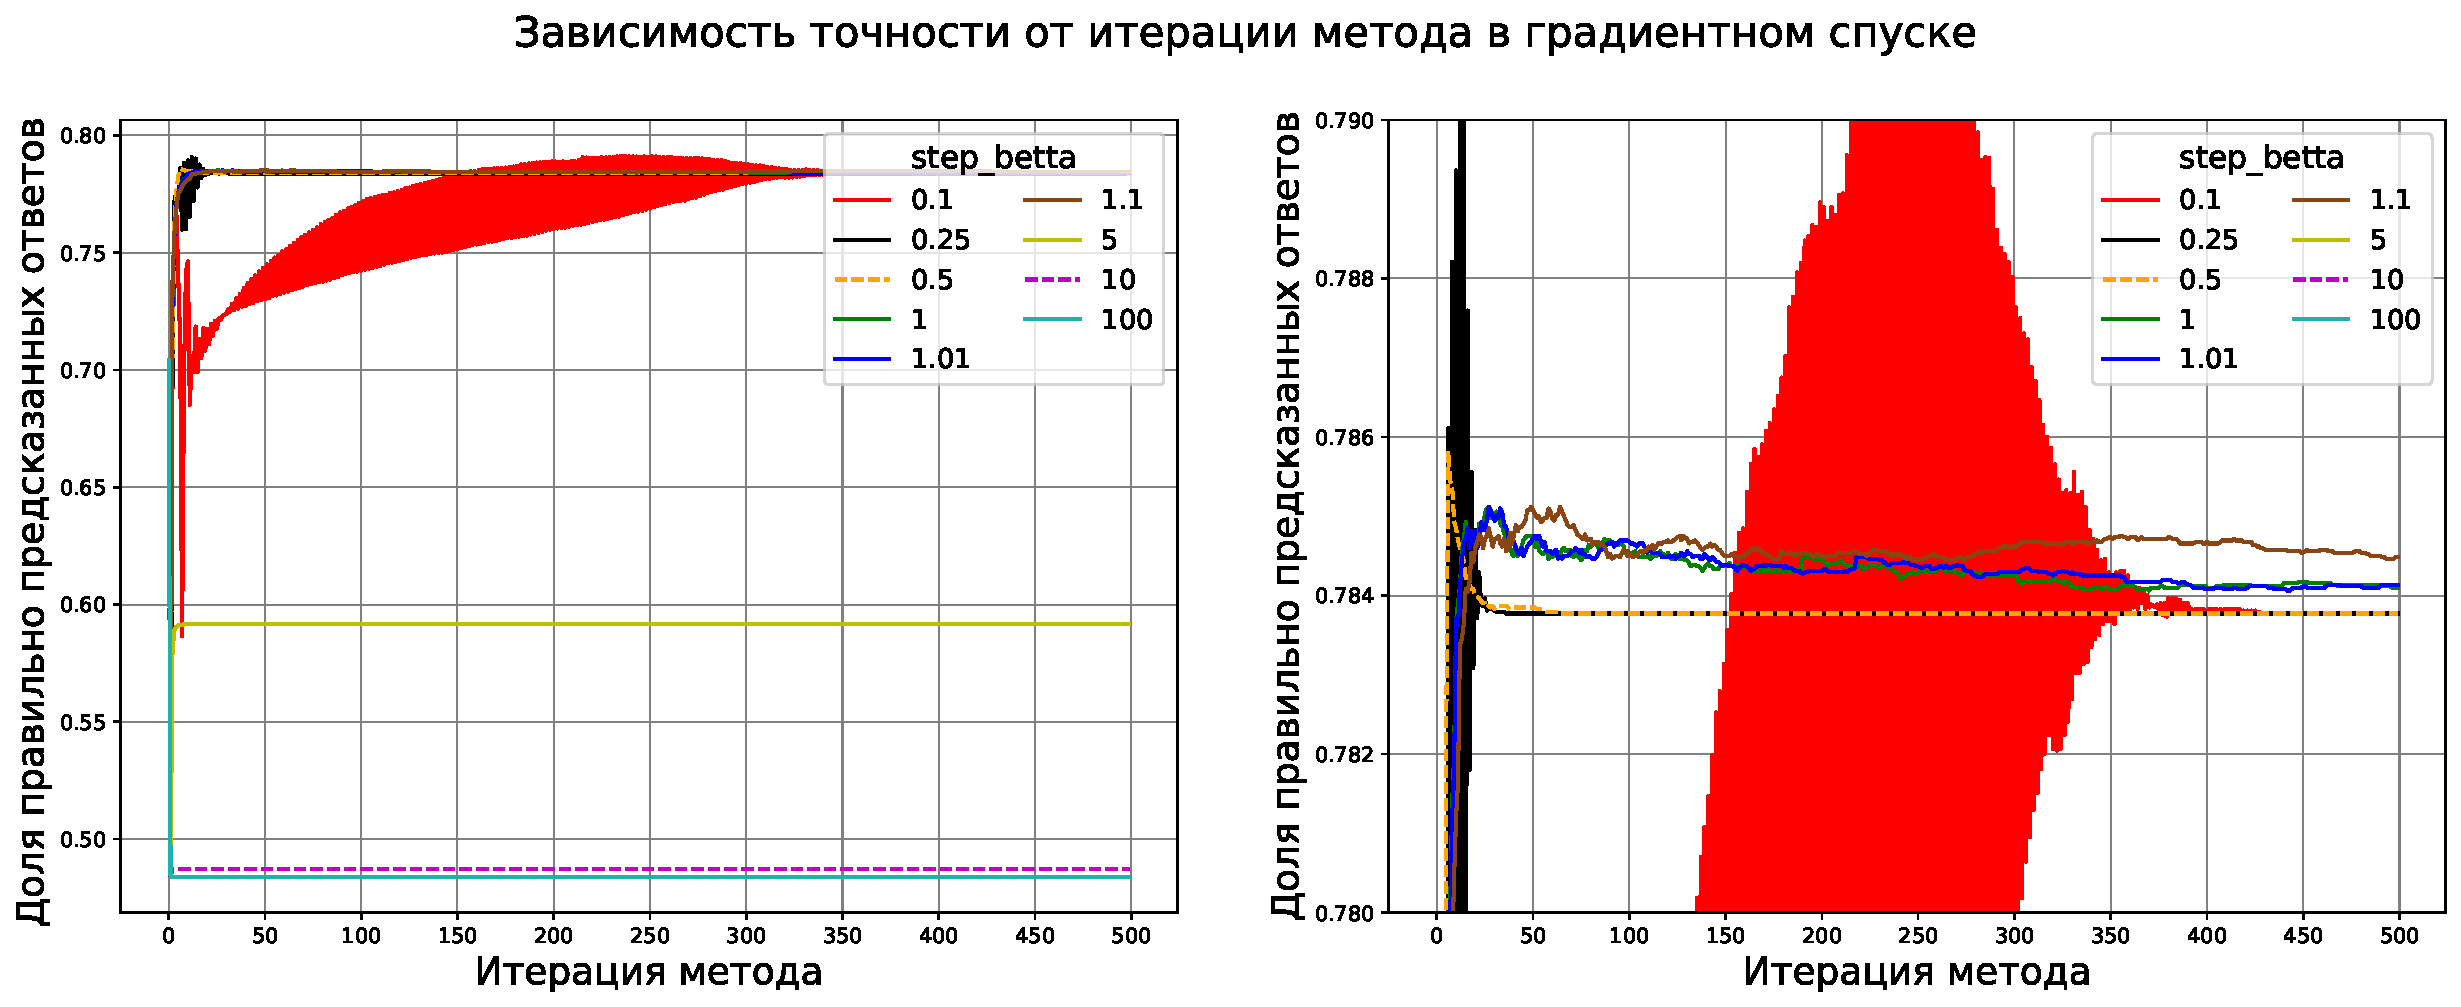
\includegraphics[width=15cm]{TASK2 step_betta accuracy.pdf}
    \caption{Точность в градиентном спуске при различных параметрах $\beta$}
    \label{fig:step_betta_accuracy}
\end{figure}

% бетта для стохастичесого
\begin{figure}[H]
    \centering
    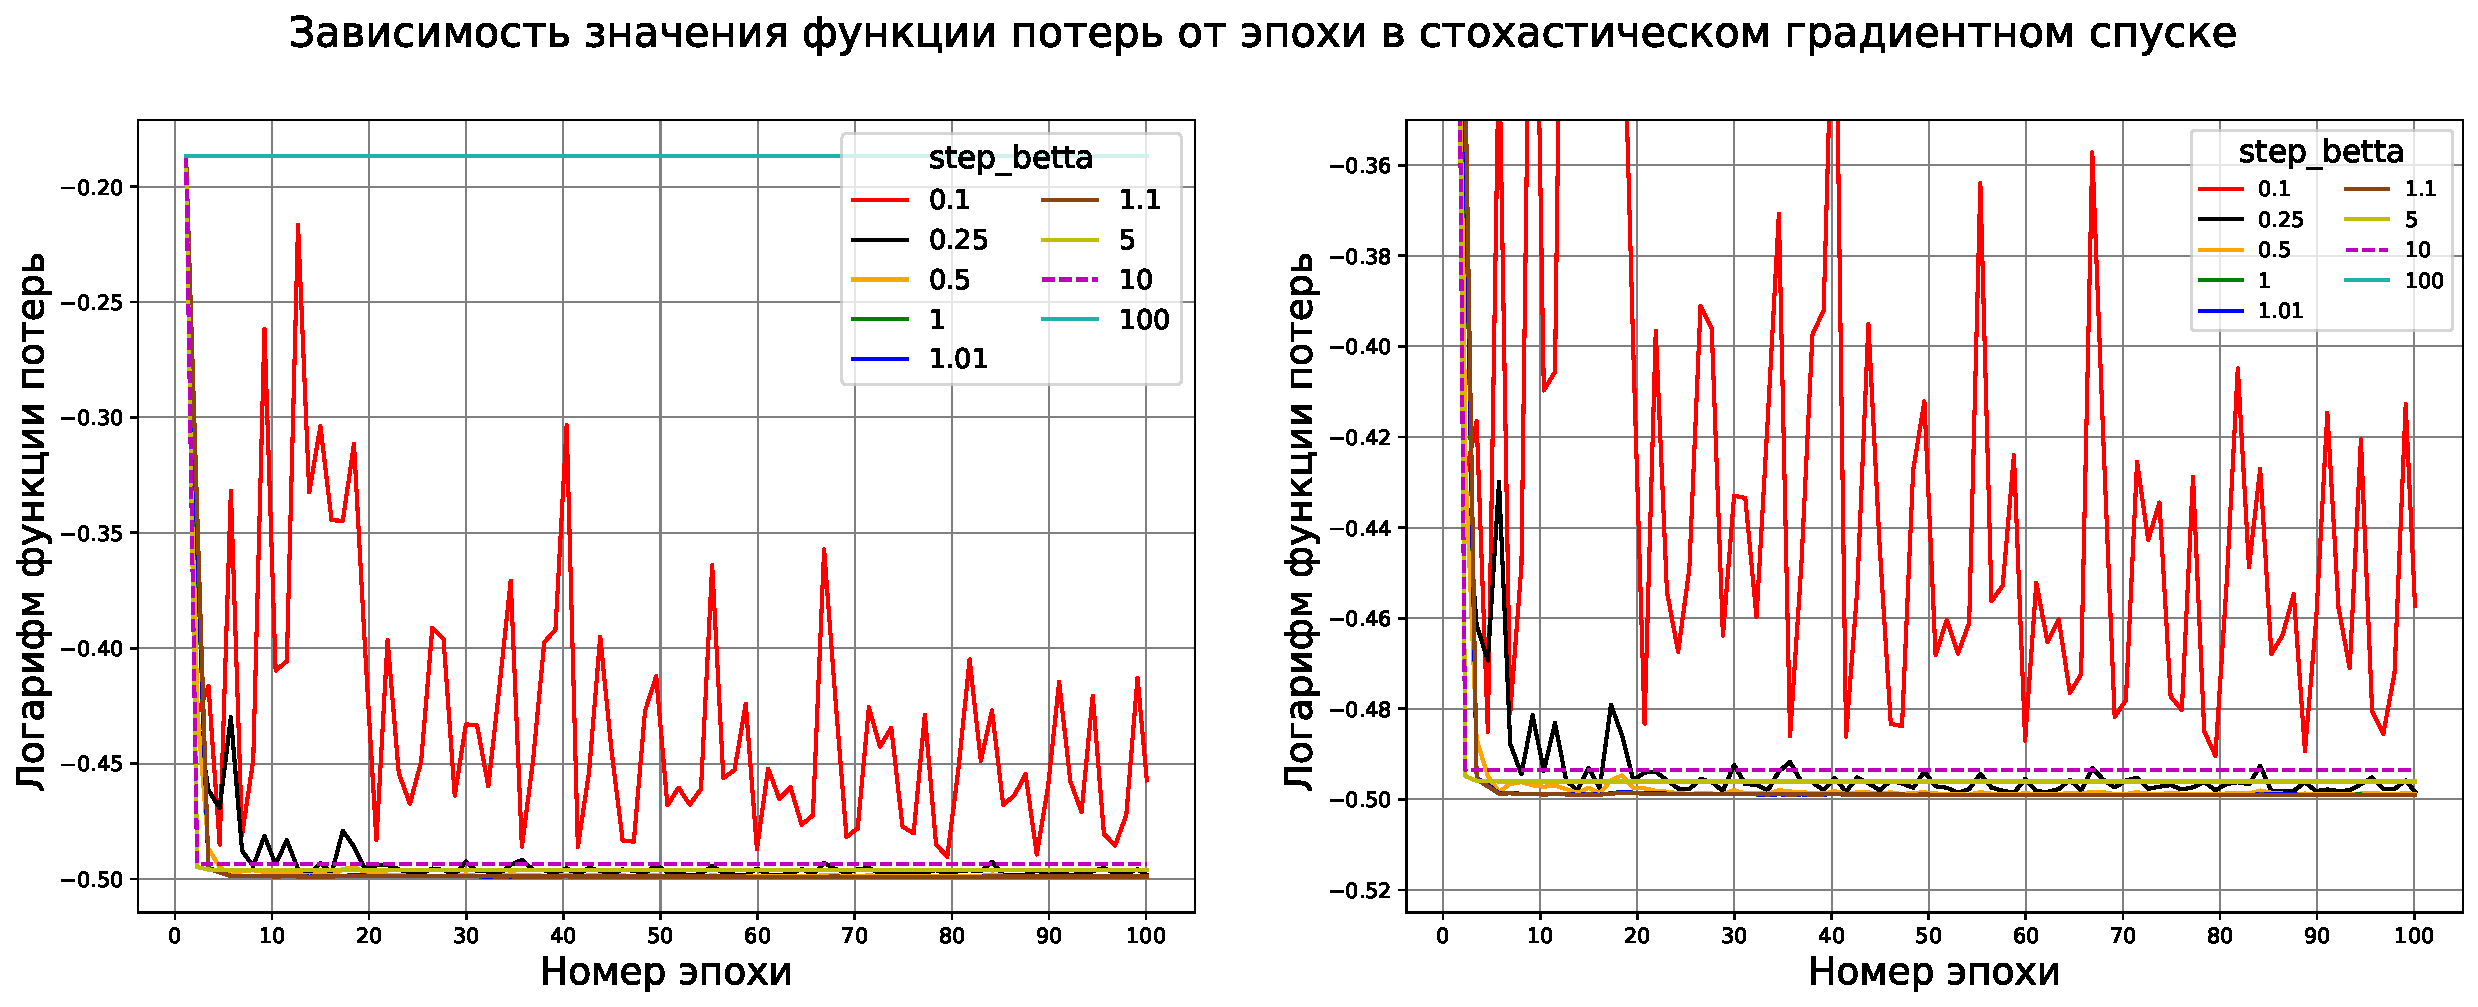
\includegraphics[width=15cm]{TASK2 step_betta loss SGDClassifier.pdf}
    \caption{Функция потерь в стохастическом градиентном спуске при различных параметрах $\beta$}
    \label{fig:step_betta_loss_SGDC}
\end{figure}
\begin{figure}[H]
    \centering
    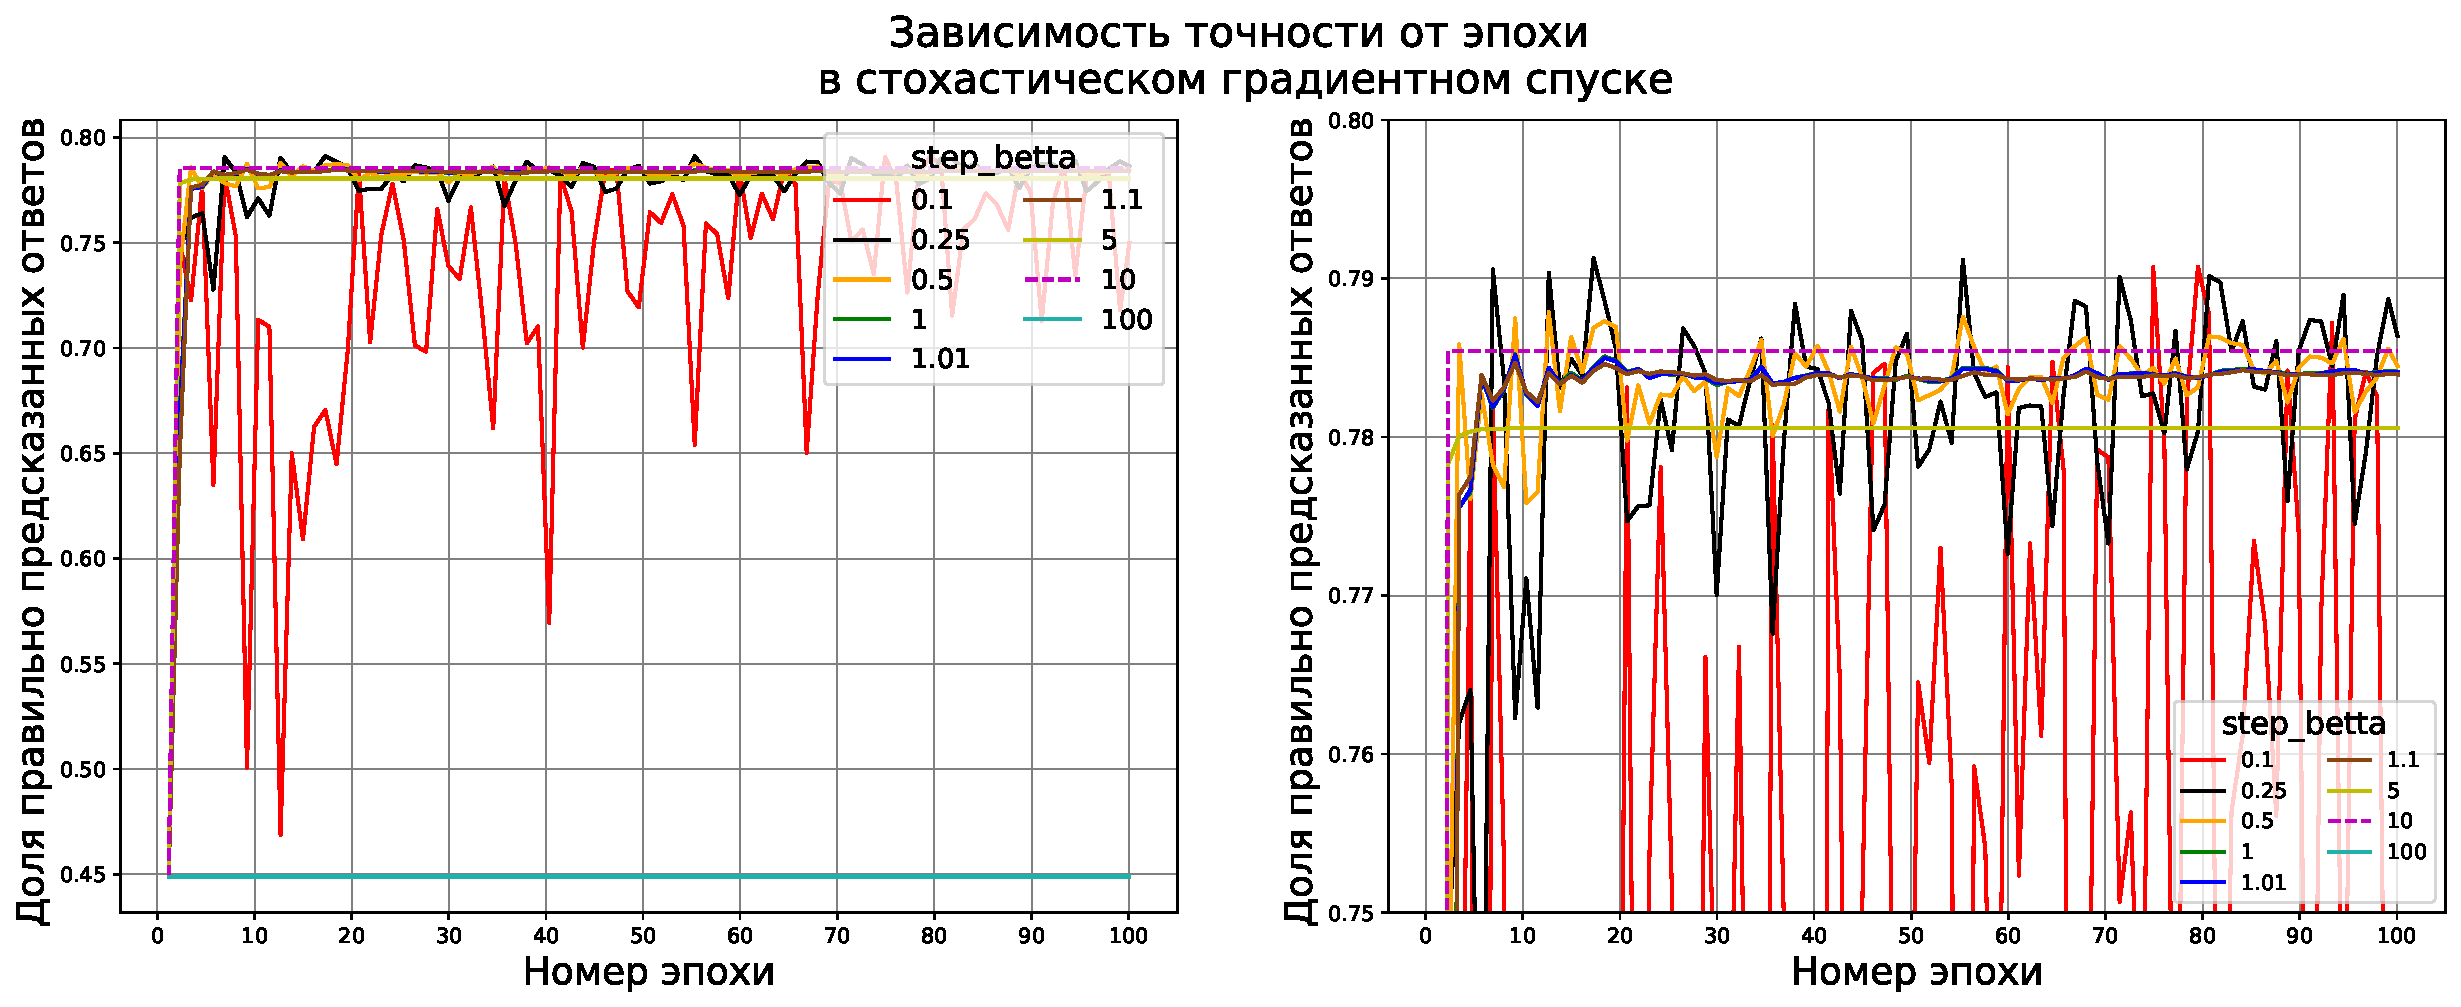
\includegraphics[width=15cm]{TASK2 step_betta accuracy SGDClassifier.pdf}
    \caption{Точность в стохастическом градиентном спуске при различных параметрах $\beta$}
    \label{fig:step_betta_accuracy_SGDC}
\end{figure}

\item
Исследуем зависимость от начального приближения. 


% веса в градиентном
\begin{figure}[H]	
    \begin{minipage}{8cm}
        \centering
        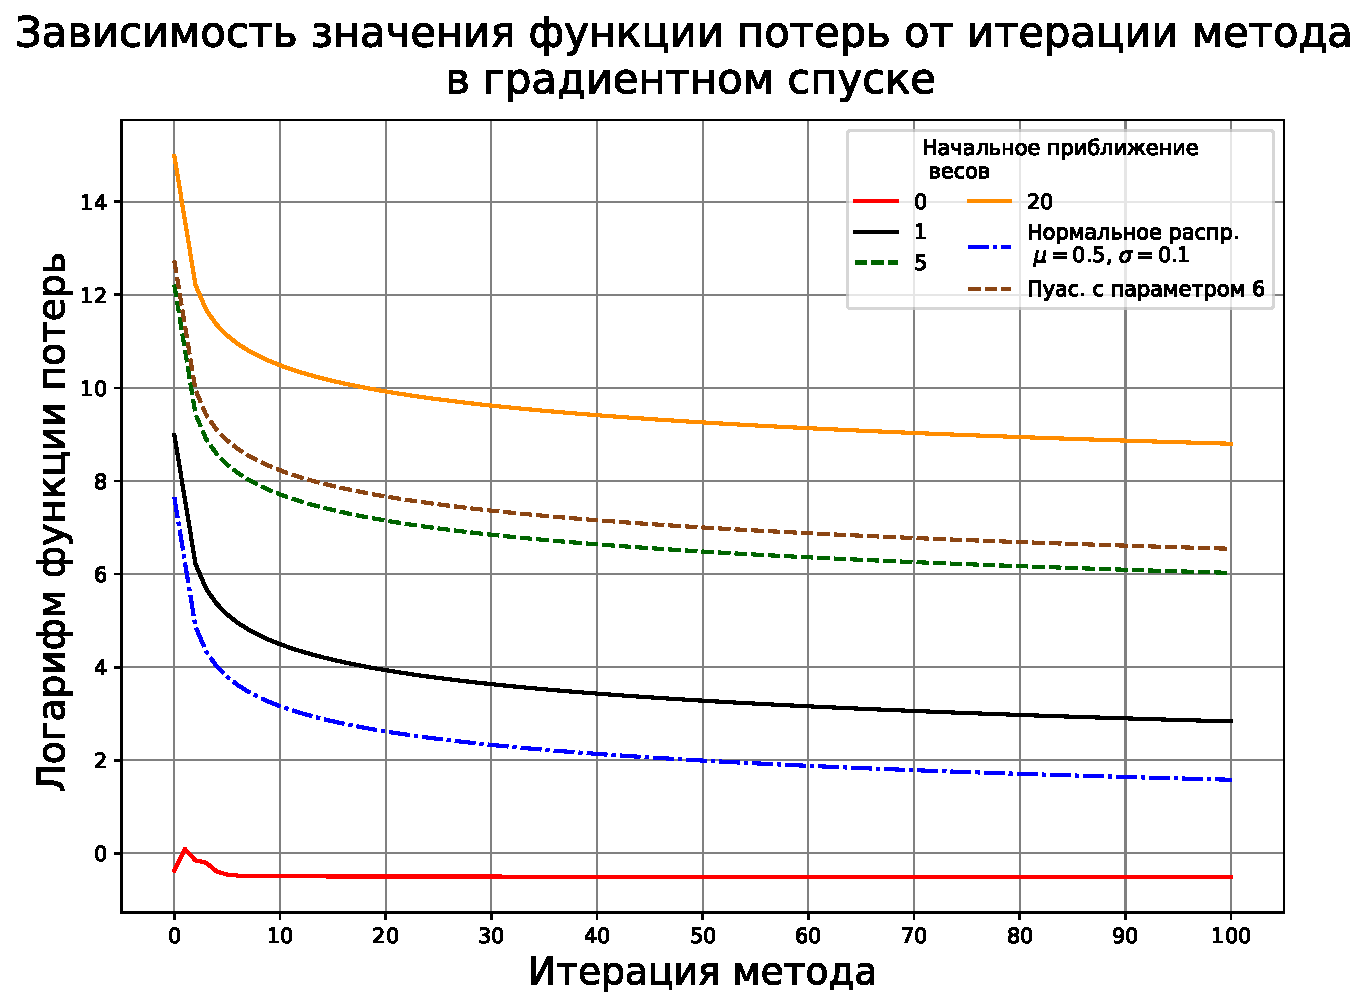
\includegraphics[scale=0.35]{TASK2 weights loss.pdf}
        \caption{Функция потерь при различных начальных приближениях}
        \label{fig:weights_loss}
    \end{minipage}
	\begin{minipage}{8cm}
		\centering
		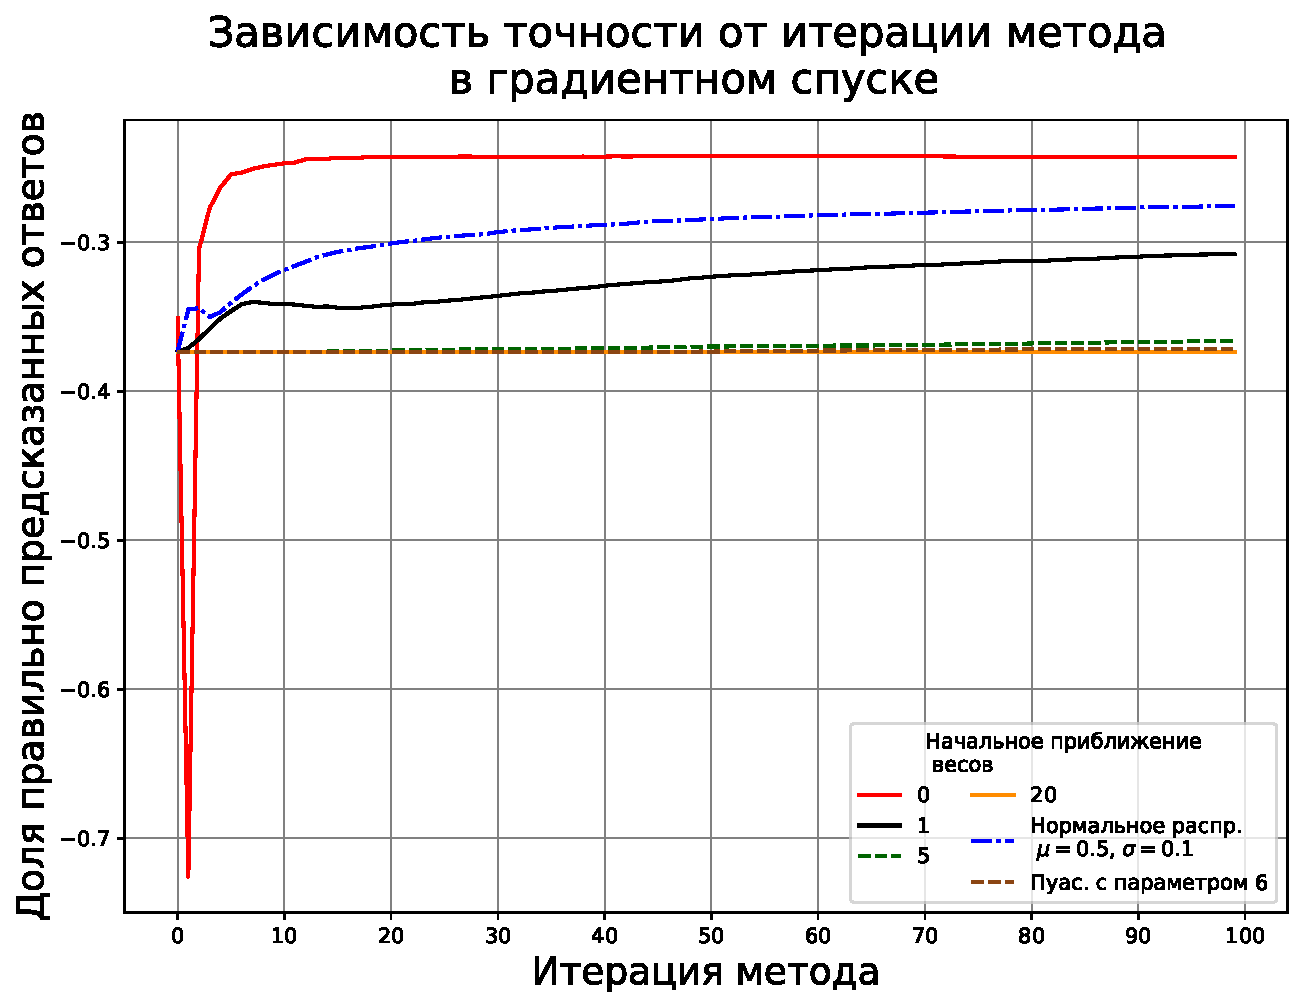
\includegraphics[scale=0.35]{TASK2 weights accuracy.pdf}
		\caption{Точность при различных начальных приближениях}
		\label{fig:weights_accuracy}
	\end{minipage}
\end{figure}



Начальные приближения весов исследованы в следующих вариантах: 

\begin{itemize}
  \item Одинаковые веса со значениями 0, 1, 5, 20;
  \item Нормальное распределение с параметрами $\mu=0.5$, $\sigma=0.1$;
  \item Пуассоновское распределение с параметром 6.
\end{itemize}

Лучший результат дает начальное нулевое приближение весов (градиентный спуск: рис. \ref{fig:weights_loss}, \ref{fig:weights_accuracy}, стохастический градиентный спуск: рис. \ref{fig:weights_loss_SGD}, \ref{fig:weights_accuracy_SGD}). При этом видно, что начальное приближене весом на поведение стохастического градиентного спуска не оказывает такого влияния, как на градиентный спуск. Далее используется такое приближение, если не оговорено другое.

% веса в стохастическом
\begin{figure}[H]	
    \centering
    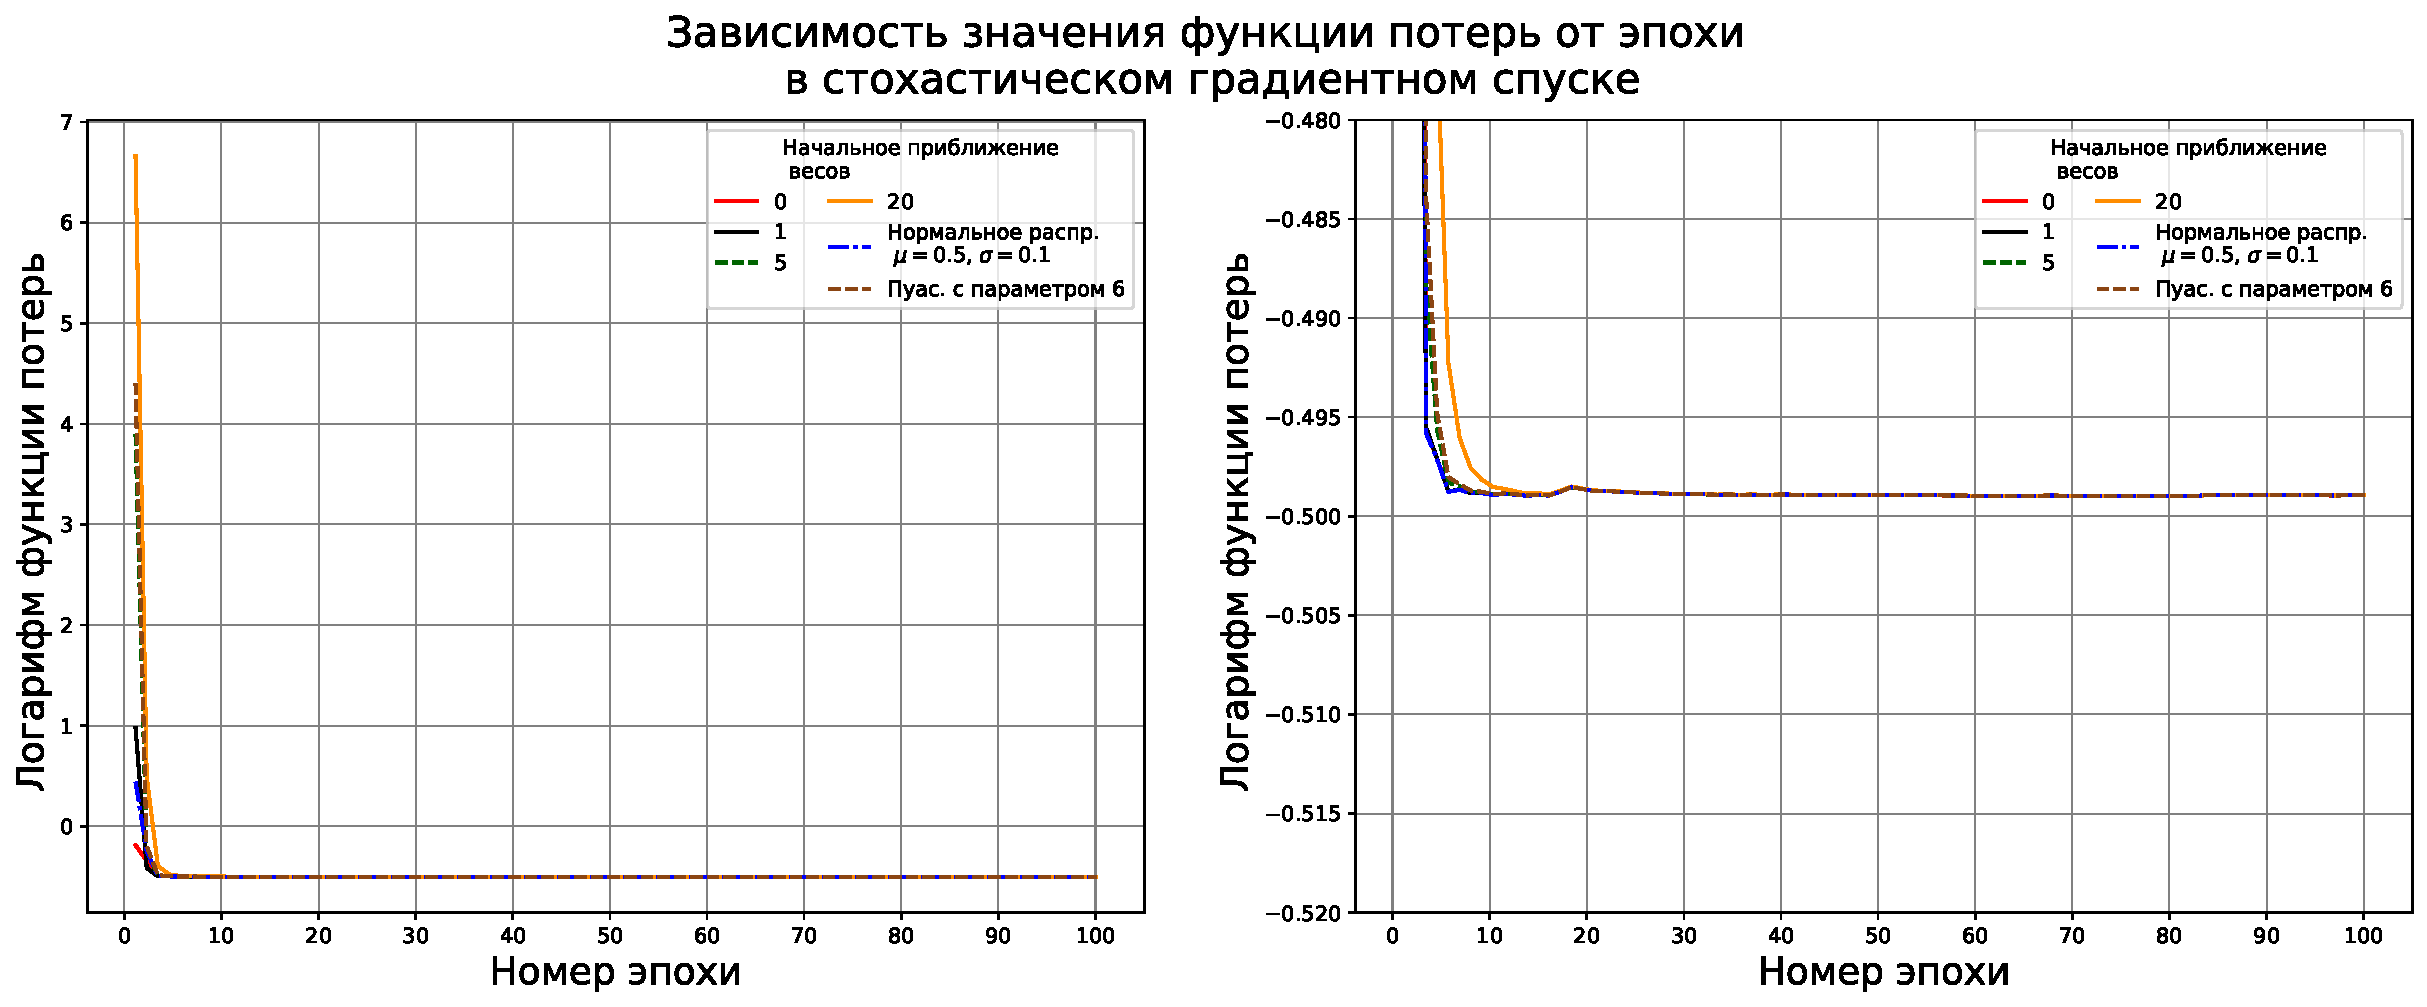
\includegraphics[width=15cm]{TASK2 weights loss SGD.pdf}
    \caption{Функция потерь в стохастическом градиентном спуске при различных начальных приближениях}
    \label{fig:weights_loss_SGD}
\end{figure}
\begin{figure}[H]
	\centering
	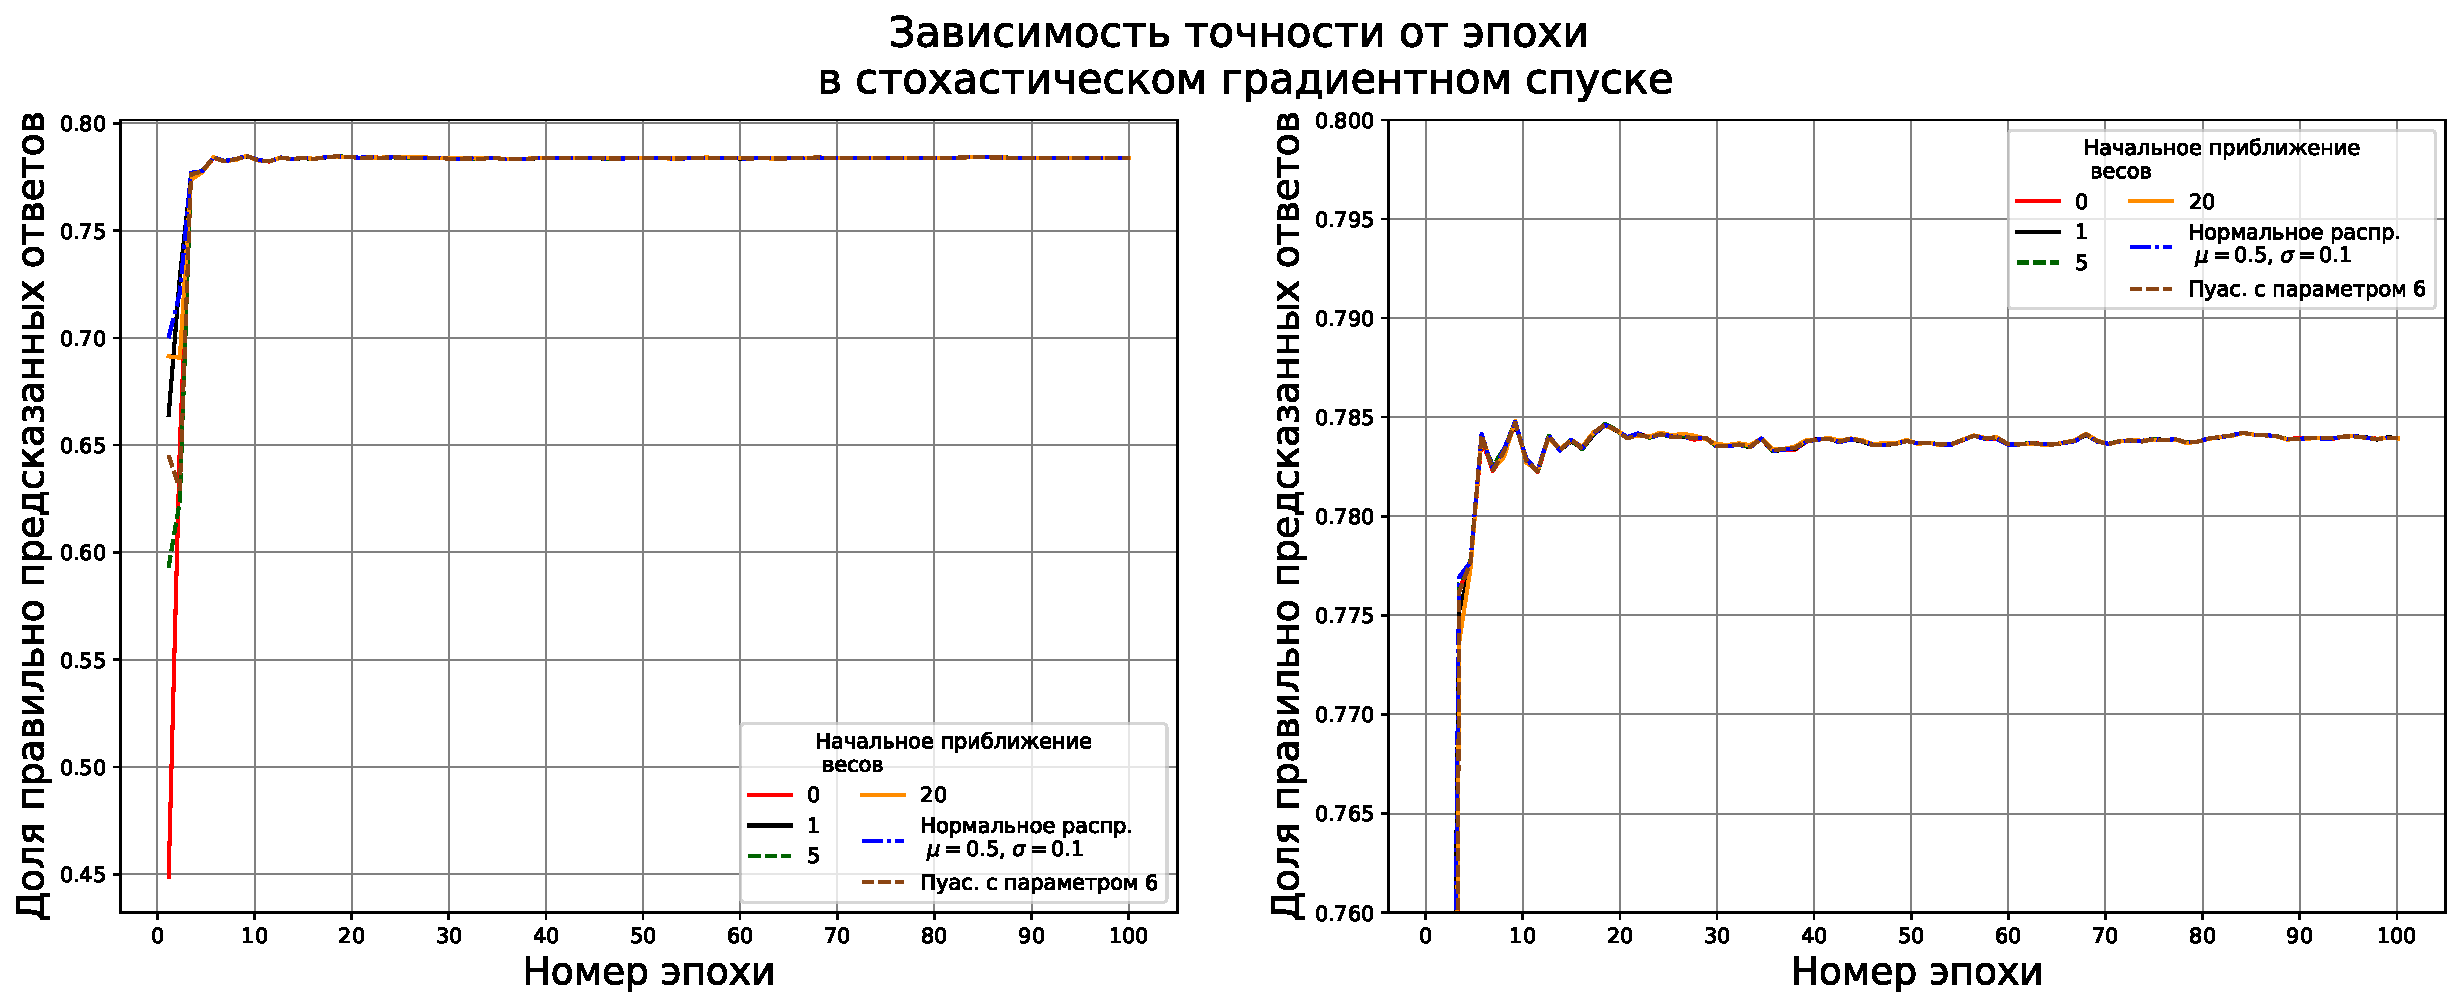
\includegraphics[width=15cm]{TASK2 weights accuracy SGD.pdf}
	\caption{Точность в стохастическом градиентном спуске при различных начальных приближениях}
	\label{fig:weights_accuracy_SGD}
\end{figure}

\item Для стохастического градиентного спуска исследуем его поведение в зависимости от параметра batch\_size. 

Значения размера подвыборки batch\_size перебираются по сетке: \{500, 1000, 5000, 10000, 25000, 50000, 100000\}. При меньших размерах подвыборки заметны колебания функции потерь и точности, а при больших – более низкие значения точности (рис. \ref{fig:batch_loss_SGD}, \ref{fig:batch_accuracy_SGD}). Далее, если не оговорено другое, используется batch\_size = 10000.


\end{itemize}


% бач сайз
\begin{figure}[H]
	\centering
	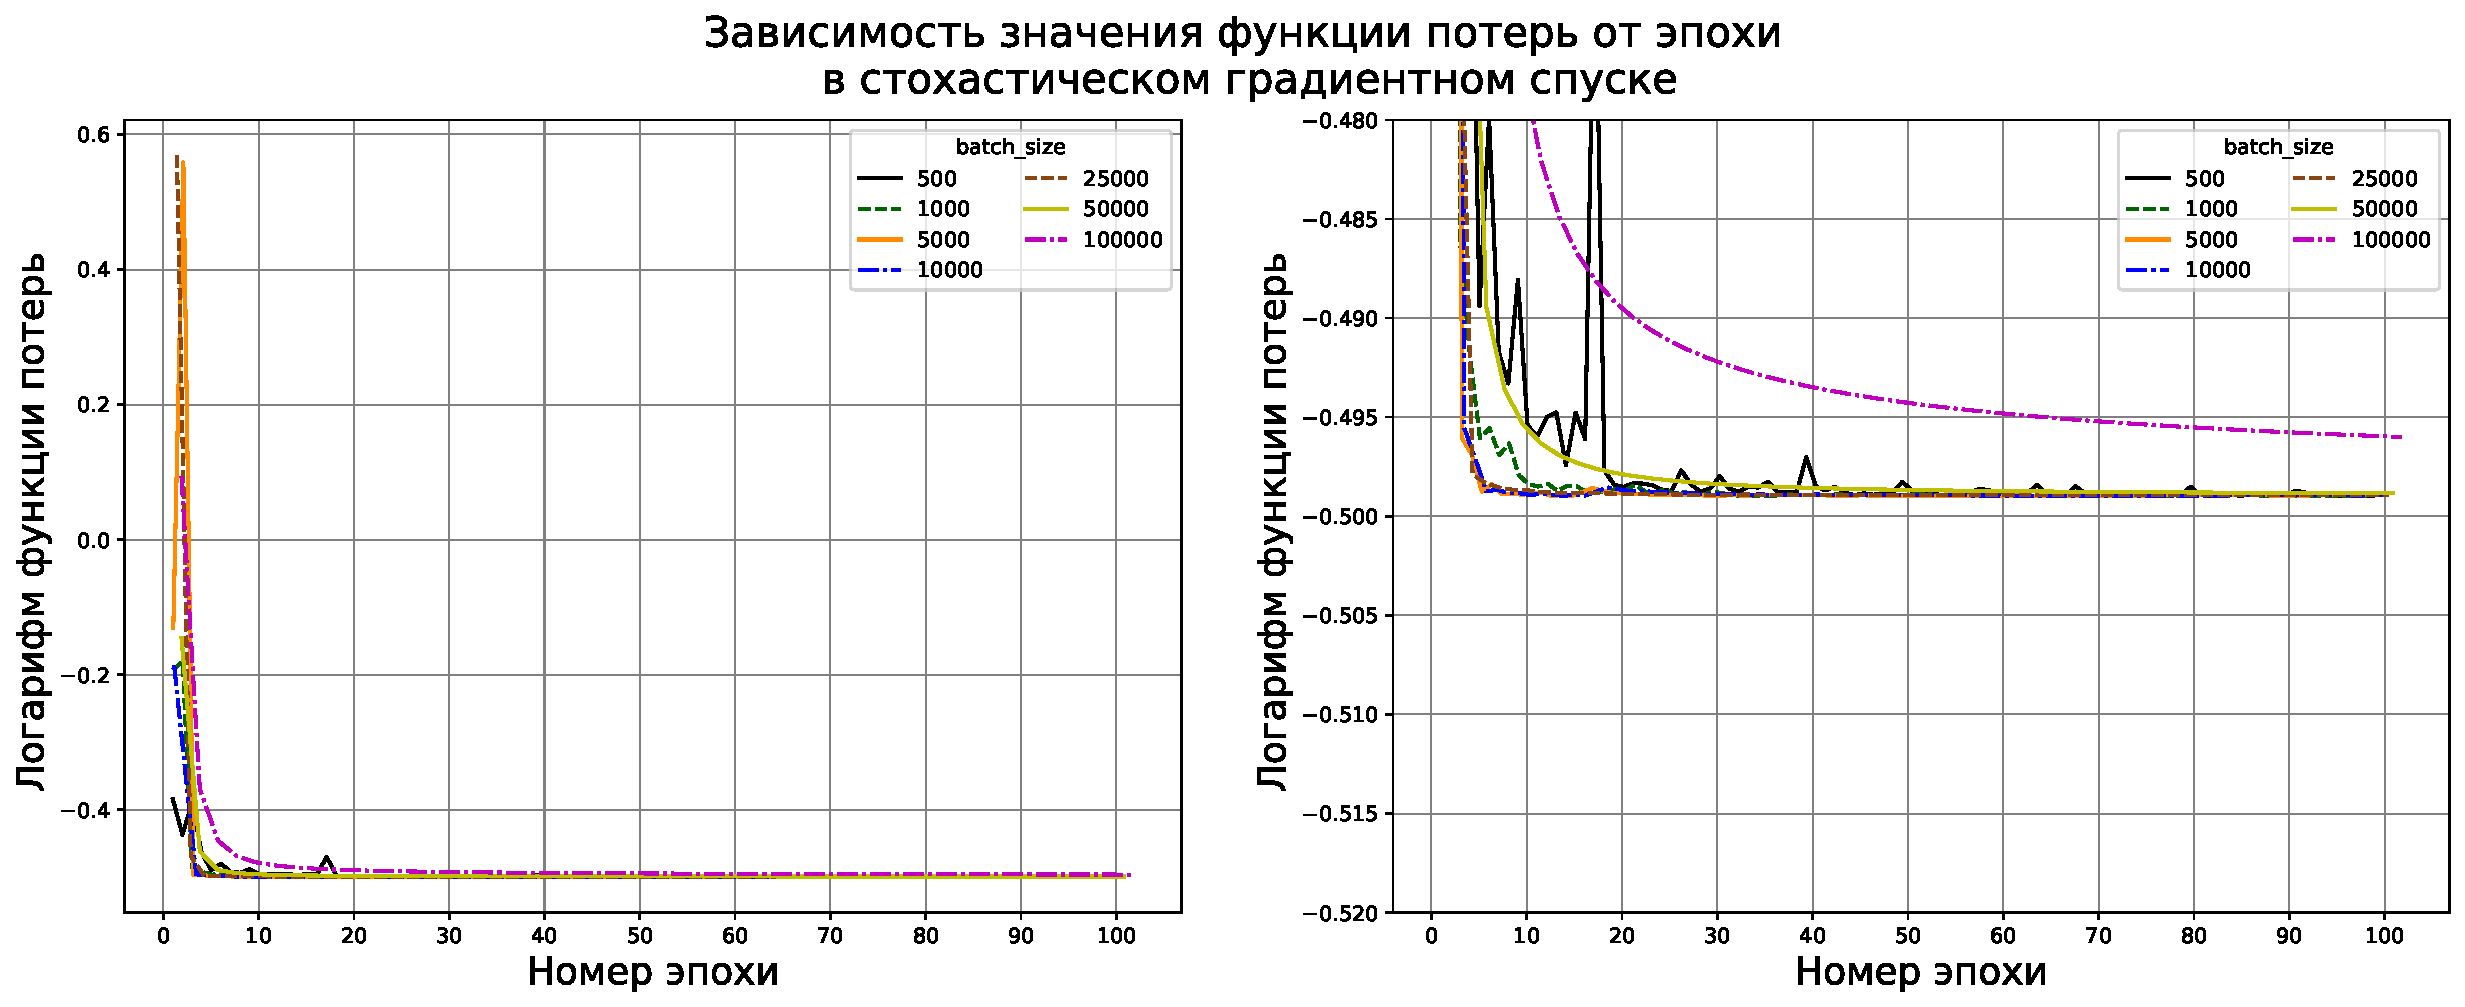
\includegraphics[width=15cm]{TASK2 batch loss SGD.pdf}
	\caption{Функция потерь в стохастическом градиентном спуске при различных batch\_size}
	\label{fig:batch_loss_SGD}
\end{figure}
\begin{figure}[H]
	\centering
	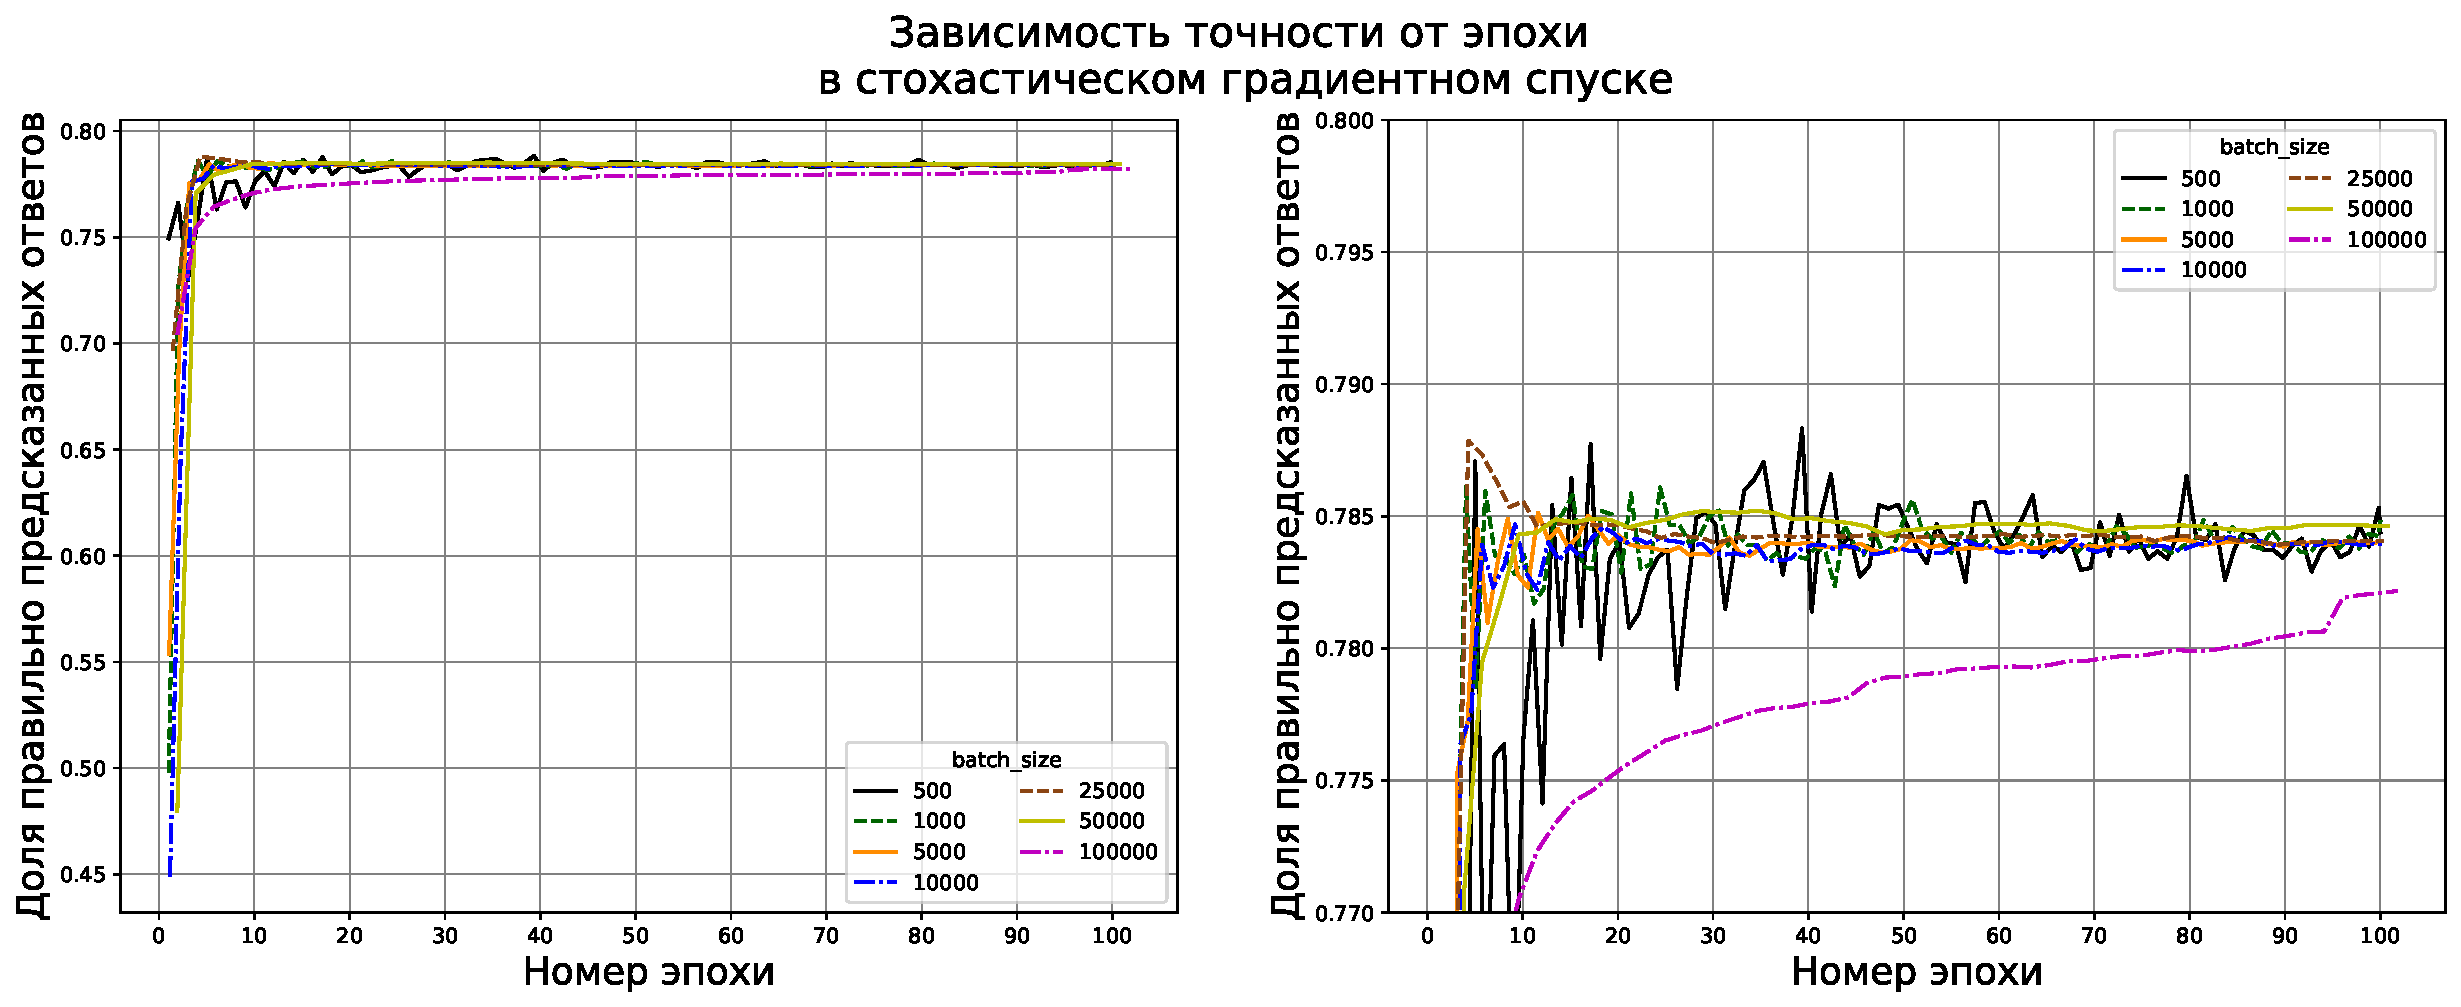
\includegraphics[width=15cm]{TASK2 batch accuracy SGD.pdf}
	\caption{Точность в стохастическом градиентном спуске при различных batch\_size}
	\label{fig:batch_accuracy_SGD}
\end{figure}

%ССЫЛКИ НА ГРАФИКИ \ref{fig:step_alpfa_loss_SGDC}, \ref{fig:step_alpfa_accuracy_SGDC}, \ref{fig:step_betta_loss_SGDC}, \ref{fig:step_betta_accuracy_SGDC}, \ref{fig:weights_loss_SGD}, \ref{fig:weights_accuracy_SGD}, \ref{fig:batch_loss_SGD}, \ref{fig:batch_accuracy_SGD}

%ССЫЛКИ НА ГРАФИКИ \ref{fig:step_alpfa_loss}, \ref{fig:step_alpfa_accuracy}, \ref{fig:step_betta_loss}, \ref{fig:step_betta_accuracy}, \ref{fig:weights_loss}, \ref{fig:weights_accuracy}



Стохастический градиентный спуск в среднем показывает результаты лучше, чем градиентный спуск и меньше колеблется при "плохих"{ }используемых параметрах. Особенно это заметно при изменении начального приближения. При большом значении batch\_size стохастический градиентный спуск ведет себя как градиентный спуск, при небольших значениях данного параметра сильно колеблется.

\section{Расширенная предобработка}

Применим к коллекции дополнительную предобработку. Воспользуемся алгоритмом лемматизации. Данный алгоритм приводит слова к лемме — нормальной форме. После этого уберем из коллекции стоп-слова (предлоги, междометия, частицы, часто встречающиеся общеупотребительные слова). Параметр min\_df остается равным 0.0001. 

После данной обработки размерность признакового пространства уменьшилась с 16050 до 14329. На графиках \ref{fig:GDC_before_and_after}, \ref{fig:SGDC_before_and_after} видно, что благодаря данной обработке работа алгоритмов ускорилась без негативного влияния на точность.

\begin{figure}[H]
	\centering
	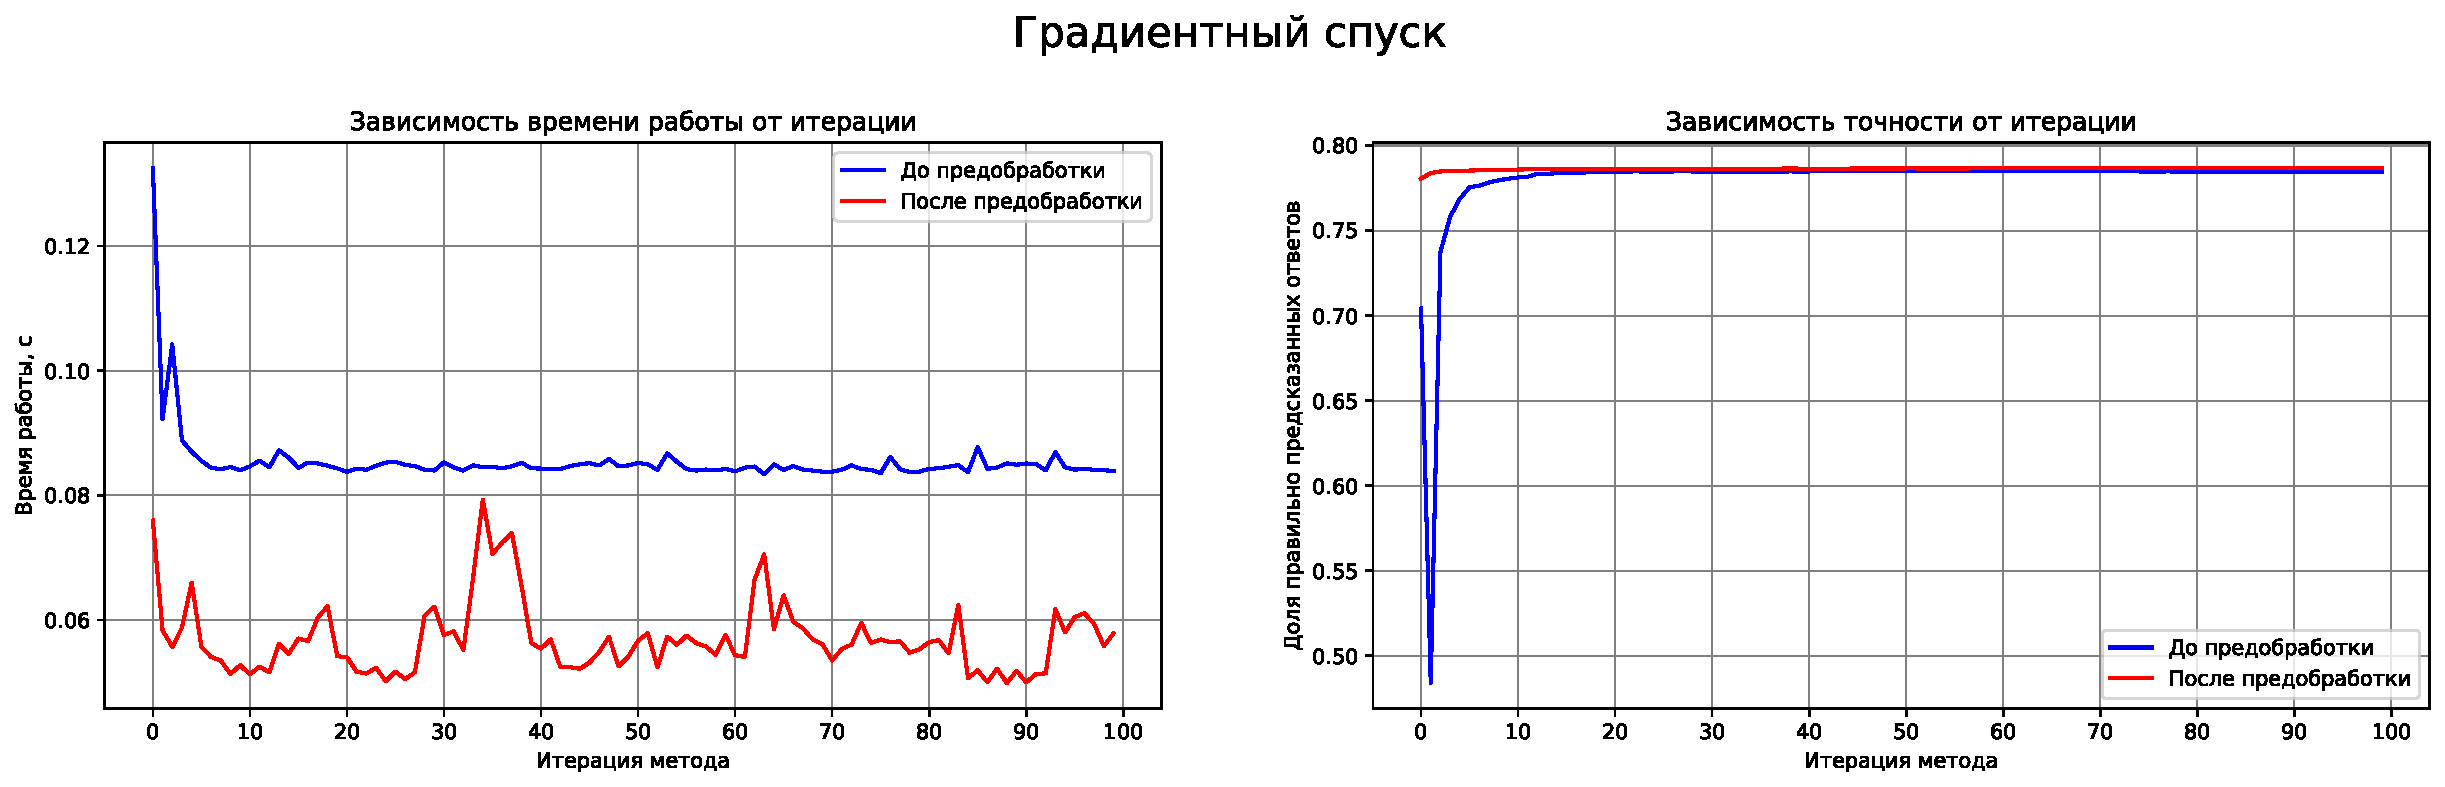
\includegraphics[width=15cm]{TASK2 GDC before and after.pdf}
	\caption{Влияние дополнительной обработки на градиентный спуск}
	\label{fig:GDC_before_and_after}
\end{figure}
\begin{figure}[H]
	\centering
	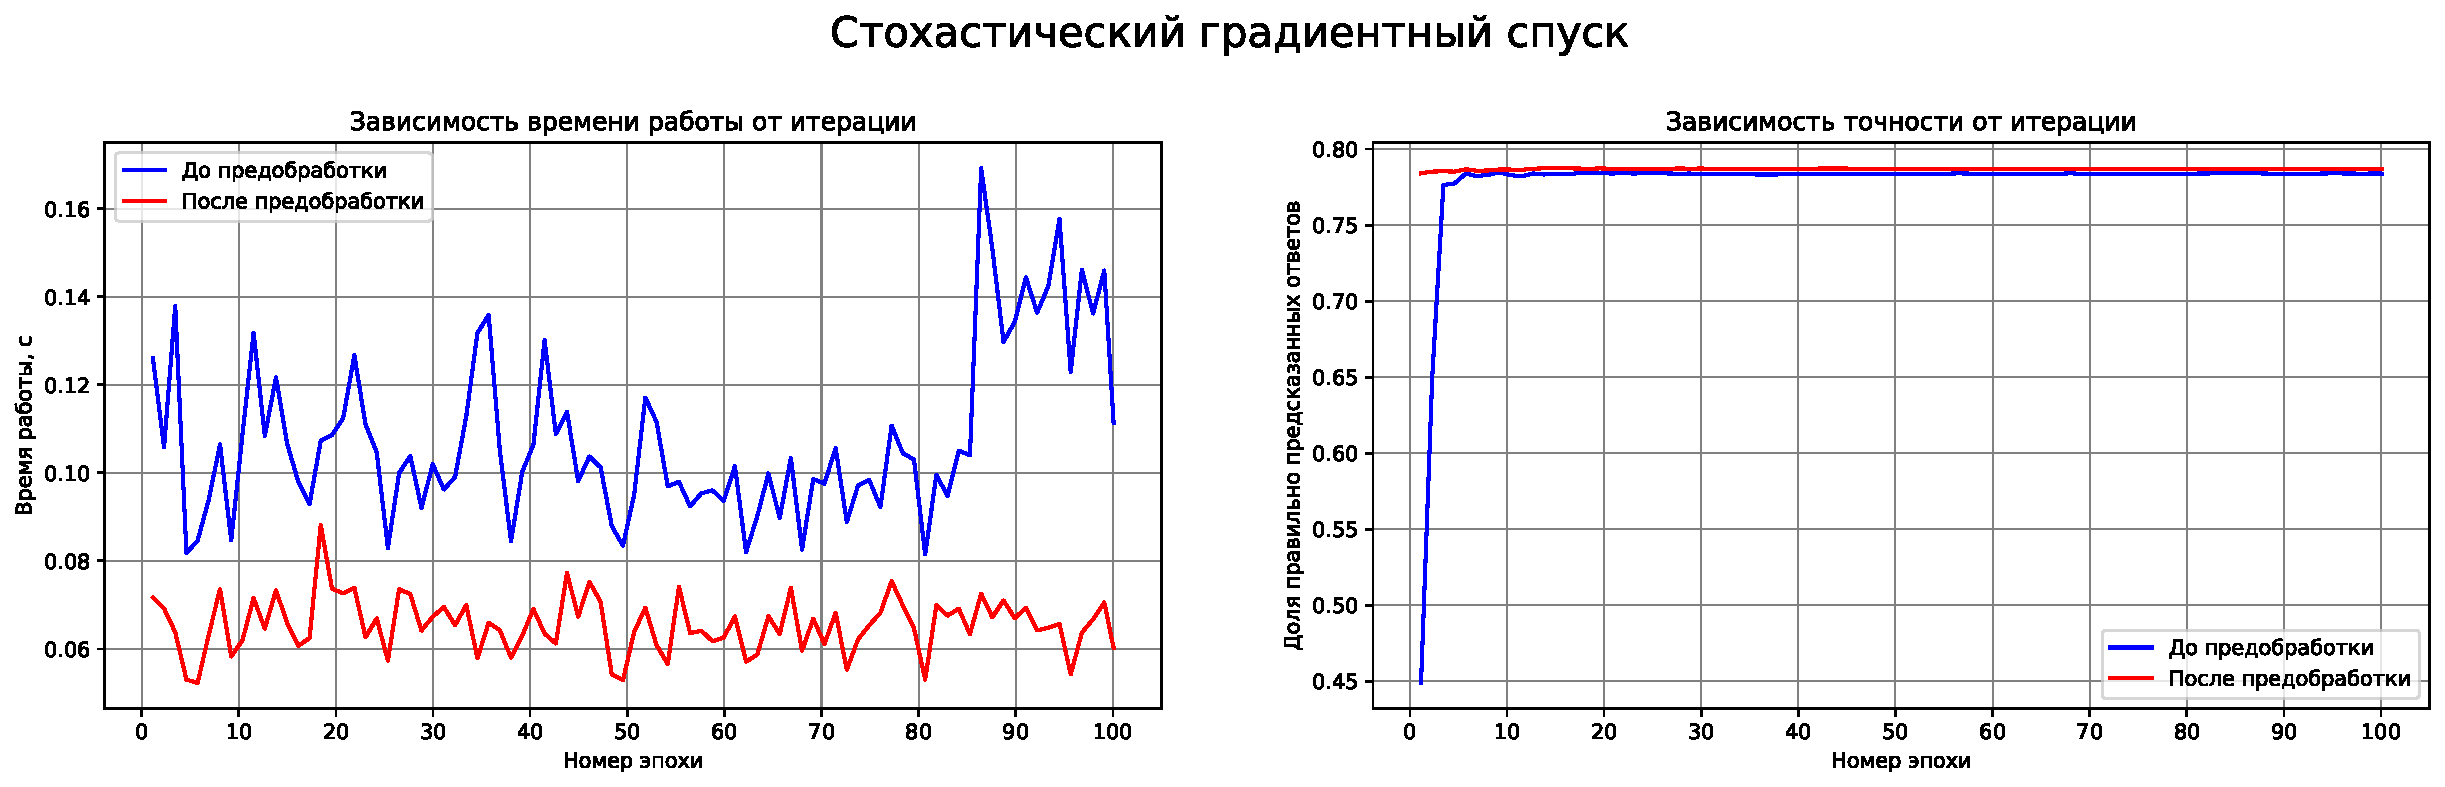
\includegraphics[width=15cm]{TASK2 SGDC before and after.pdf}
	\caption{Влияние дополнительной обработки на стохастический градиентный спуск}
	\label{fig:SGDC_before_and_after}
\end{figure}

%ССЫЛКИ НА ВЕРХНИЕ 2 - \ref{fig:GDC_before_and_after}, \ref{fig:SGDC_before_and_after}

\section{Исследование влияния способа представления коллекции на алгоритмы}

В предыдущем пункте было выяснено, что дополнительная предобработка положительно влияет на поведение методов, поэтому здесь и далее используем ее, если не оговорено другое. 

В предыдущих экспериментах выборка была представлена в виде «мешка слов» («Bag of words»). В данном эксперименте используется и другое представление: Tf-Idf, учитывающее распределение слов во всём корпусе текстов. При этом каждый документ представляется вектором длины |V|, то есть, размерность признакового пространства остается такой же (что будет подвтерждено далее графиками). Проводится сравнение скорости работы и точности методов при этих двух представлениях, при этом используется выборка с расширенной обработкой.

\begin{figure}[H]
	\centering
	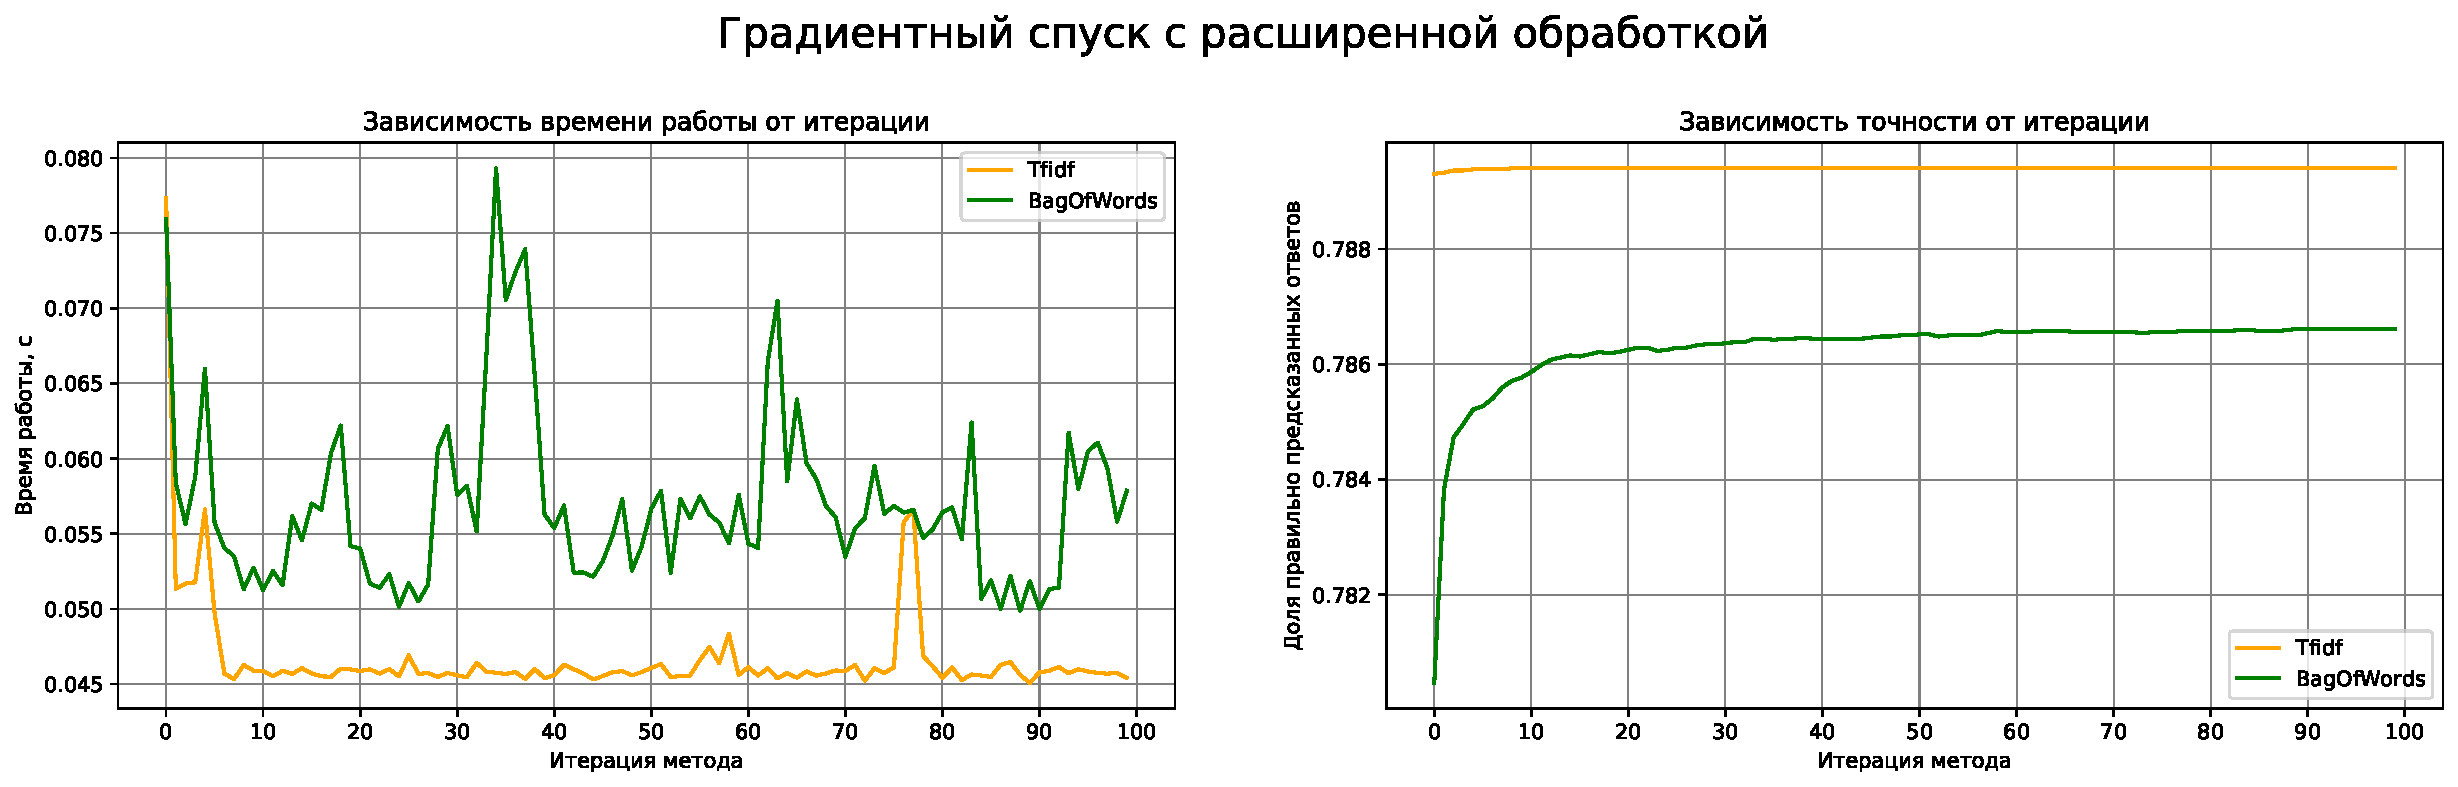
\includegraphics[width=15cm]{TASK2 GDC Tfidf.pdf}
	\caption{Влияние способа представления на градиентный спуск}
	\label{fig:GDC_Tfidf}
\end{figure}
\begin{figure}[H]
	\centering
	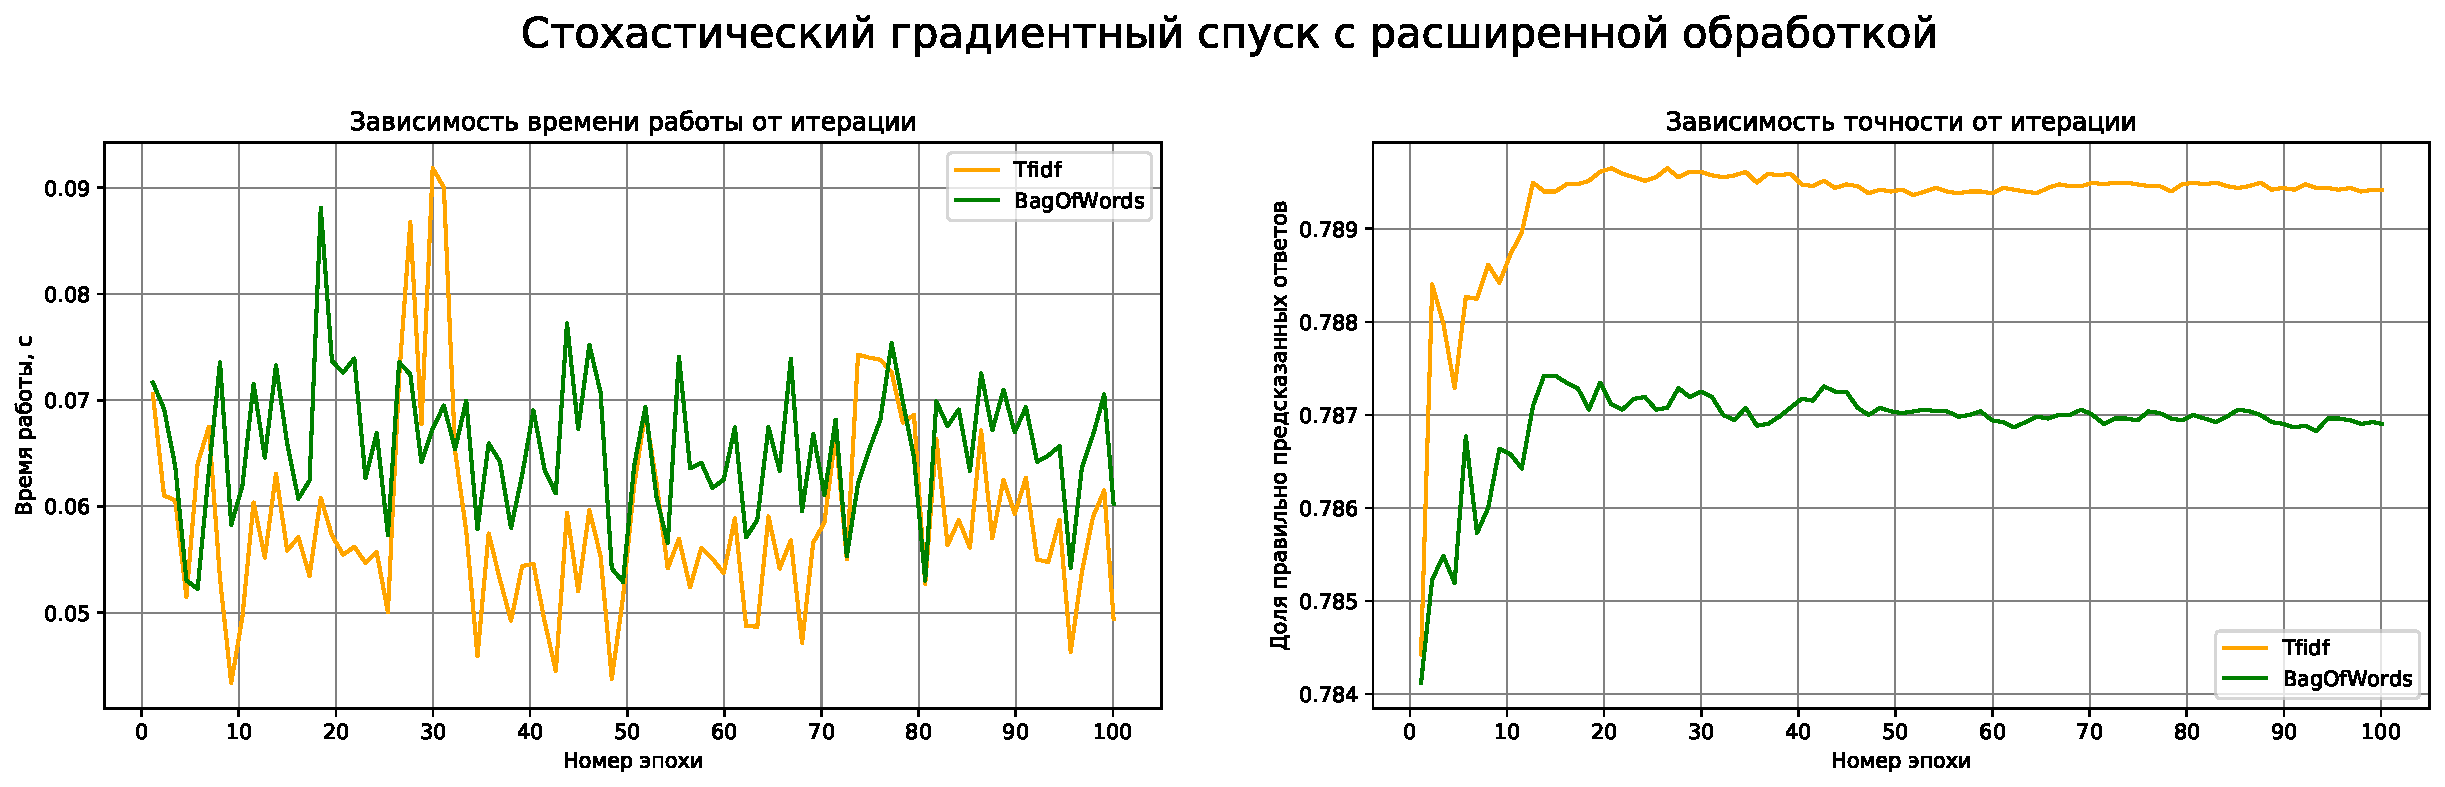
\includegraphics[width=15cm]{TASK2 SGDC Tfidf.pdf}
	\caption{Влияние способа представления на стохастический градиентный спуск}
	\label{fig:SGDC_Tfidf}
\end{figure}

При сравнении этих двух методом получены результаты, представленные на графиках (рис. \ref{fig:GDC_Tfidf}, \ref{fig:SGDC_Tfidf}). Представление в виде Tf-Idf дает лучшую точность и меньшее время работы, чем представление в виде Bag of words. 

\section{Изменение параметров min\_df и max\_df конструкторов}

Изменение параметров min\_df и max\_df конструкторов позволяет уменьшить размерность признакового пространства, и, как следствие, уменьшить время работы алгоритма, а также в некоторых случаях улучшить качество работы. 

Параметр max\_df используется для удаления терминов, которые появляются слишком часто, также называемых "фиксированными словами". Например, max\_df = 0.50 означает "игнорировать лексемы, которые появляются в более чем 50\% документов". Значение max\_df умолчанию 1.0, что означает "игнорировать лексемы, которые появляются в более чем 100\% документов". Параметр min\_df используется для удаления терминов, которые появляются слишком редко. Например, min\_df = 0.01 означает "игнорировать лексемы, которые появляются менее чем в 1\% документов". Значение min\_df умолчанию 1, что означает "игнорировать термины, которые  появляются менее чем в одном документе". Таким образом, значения по умолчанию не игнорируют никакие лексемы \cite{ss2}.

Ранее использовался параметр min\_df = 0.0001, уменьшивший размерность пространства с
89658 признаков до 16050. В данном эксперименте исследуется влияние параметров min\_df и max\_df на размерность признакового пространства, скорость работы алгоритмов, точность и размерность признакового пространства. При этом используется представление и Bag of words, и Tf-Idf, и используется расширенная обработка текстов.

\begin{itemize}
  \item Изменение параметра min\_df

Параметр max\_df перебирается по сетке: \{0, 0.000001, 0.00001, 0.0001, 0.001, 0.01, 0.05, 0.1\}. При этом значение min\_df остается значением по умолчанию. При увеличении данного параметра скорость работы естественным образом уменьшается (прежде всего, за счет уменьшения размерности признакового пространства) (рис. \ref{fig:min_df_BagOfWords_GD}, \ref{fig:min_df_BagOfWords_SGD}, \ref{fig:min_df_Tfidf_GD}, \ref{fig:min_df_Tfidf_SGD}). Размерность признакового пространства не меняется заметно при трех минимальных перебранных min\_df (рис. \ref{fig:min_df_size}), а на четвертом минимальном (min\_df=0.0001) скачок в размерности уже заметен, при этом, точность на всех четырех минимальных остается одинаково высокой. При дальнейшем увеличении параметра точность ухудшается. Получаем, что min\_df=0.0001 дает максимальную точность и наименьшее из других параметров, дающих такую же точность, время работы. Заметим также, что как и было сказано ранее, размерности при обоих способах представления выборки (Tf-Idf и Bag of words) одинаковы (рис. \ref{fig:min_df_size}).


\begin{figure}[H]
	\centering
	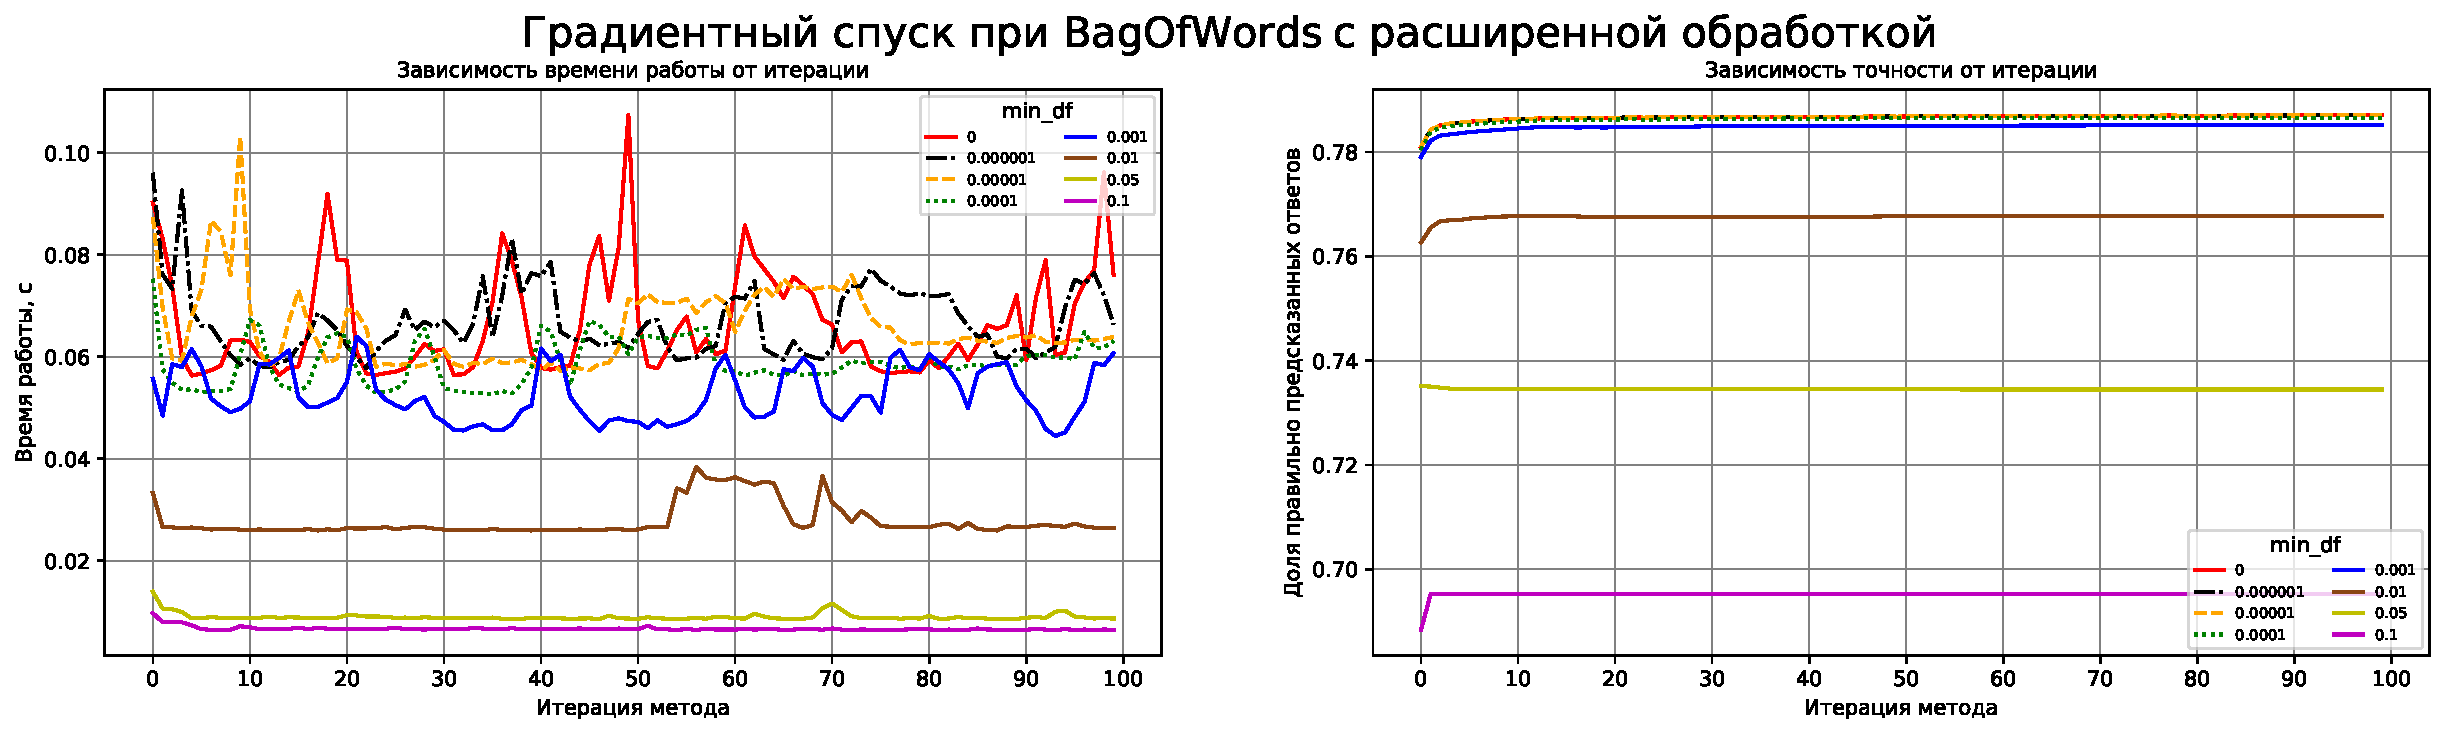
\includegraphics[width=14cm]{TASK2 min_df BagOfWords GD.pdf}
	\caption{Поведение градиентного спуска при представлении Bag Of Words и изменении параметра min\_df}
	\label{fig:min_df_BagOfWords_GD}
\end{figure}
\begin{figure}[H]
	\centering
	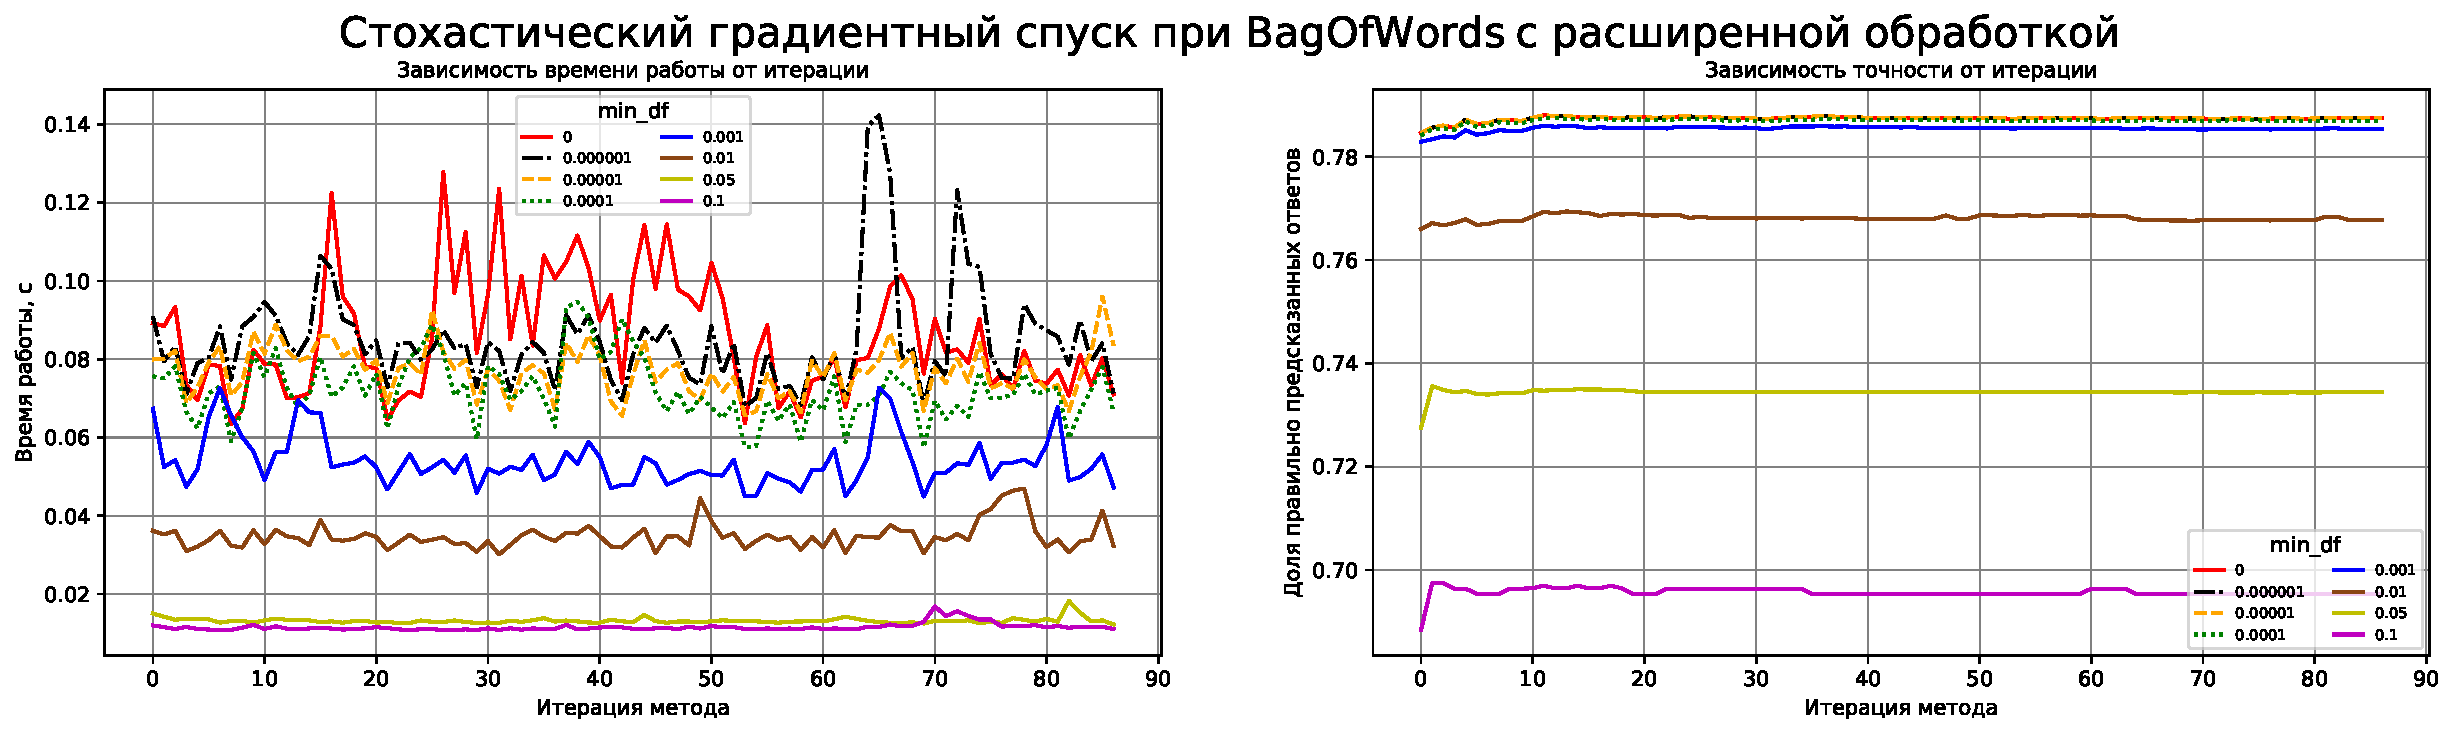
\includegraphics[width=14cm]{TASK2 min_df BagOfWords SGD.pdf}
	\caption{Поведение стохастического градиентного спуска при представлении Bag Of Words и изменении параметра min\_df}
	\label{fig:min_df_BagOfWords_SGD}
\end{figure}
\begin{figure}[H]
	\centering
	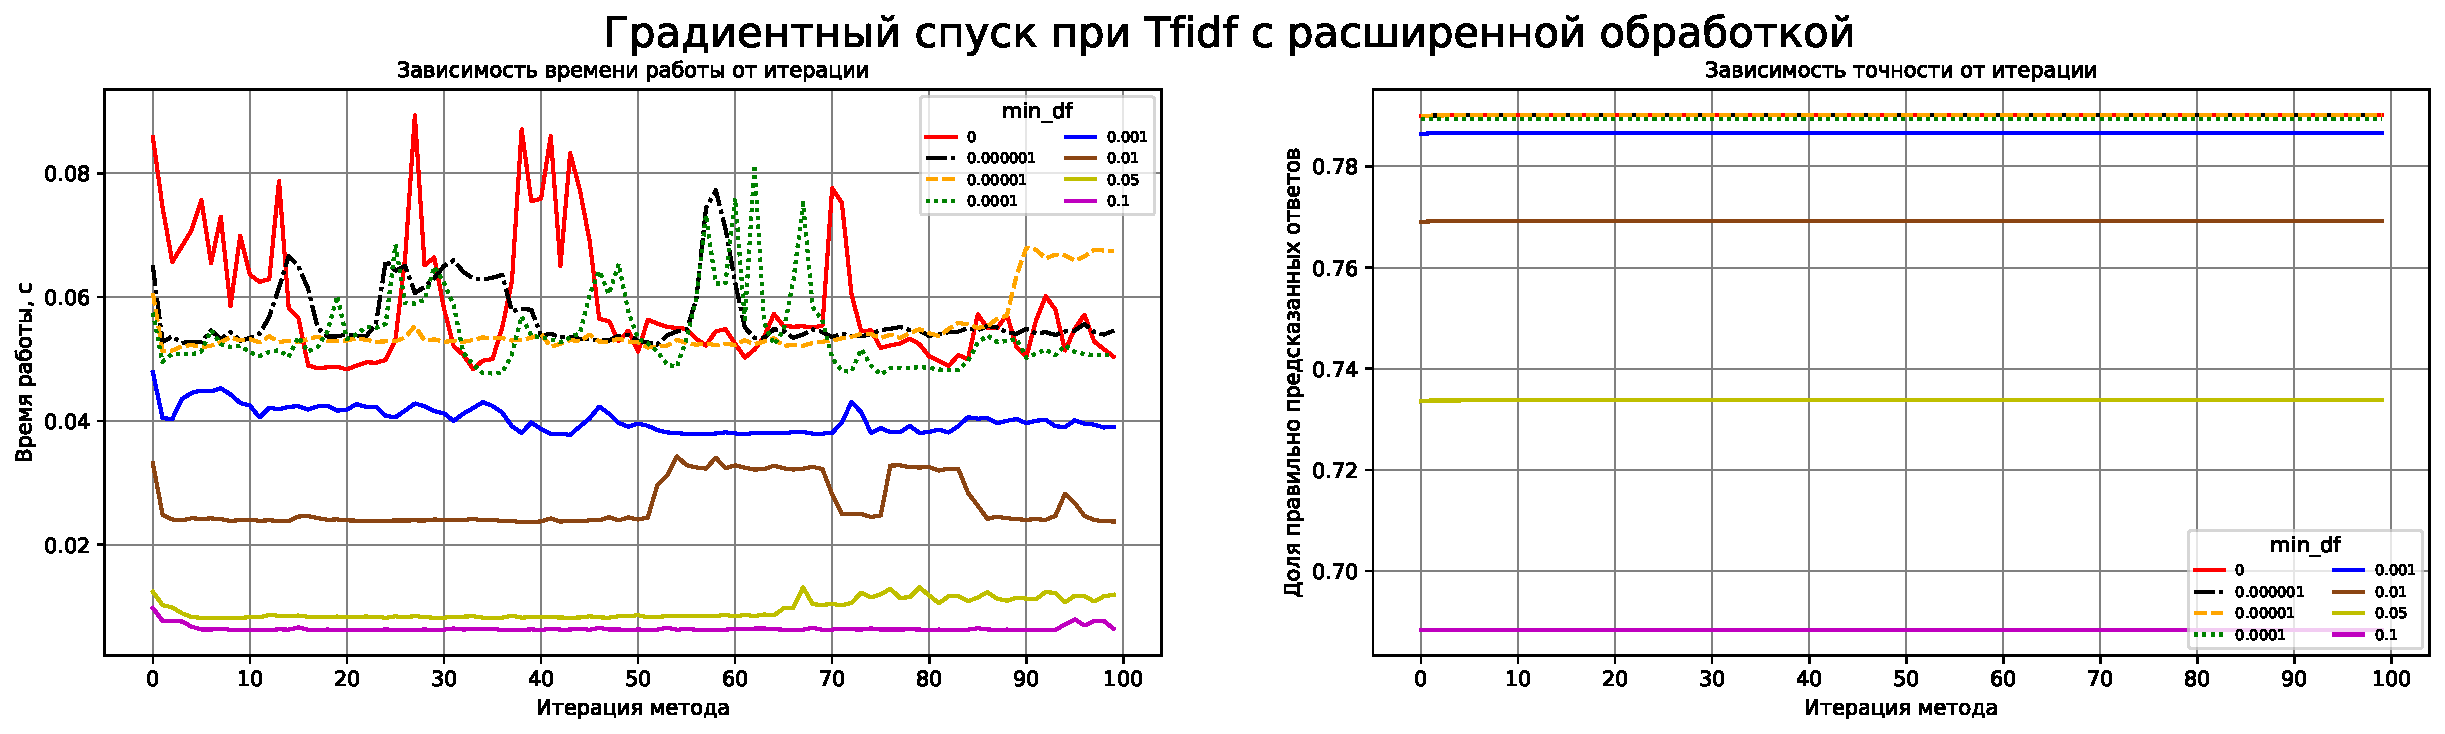
\includegraphics[width=14cm]{TASK2 min_df Tfidf GD.pdf}
	\caption{Поведение градиентного спуска при представлении Tf-Idf и изменении параметра min\_df}
	\label{fig:min_df_Tfidf_GD}
\end{figure}
\begin{figure}[H]
	\centering
	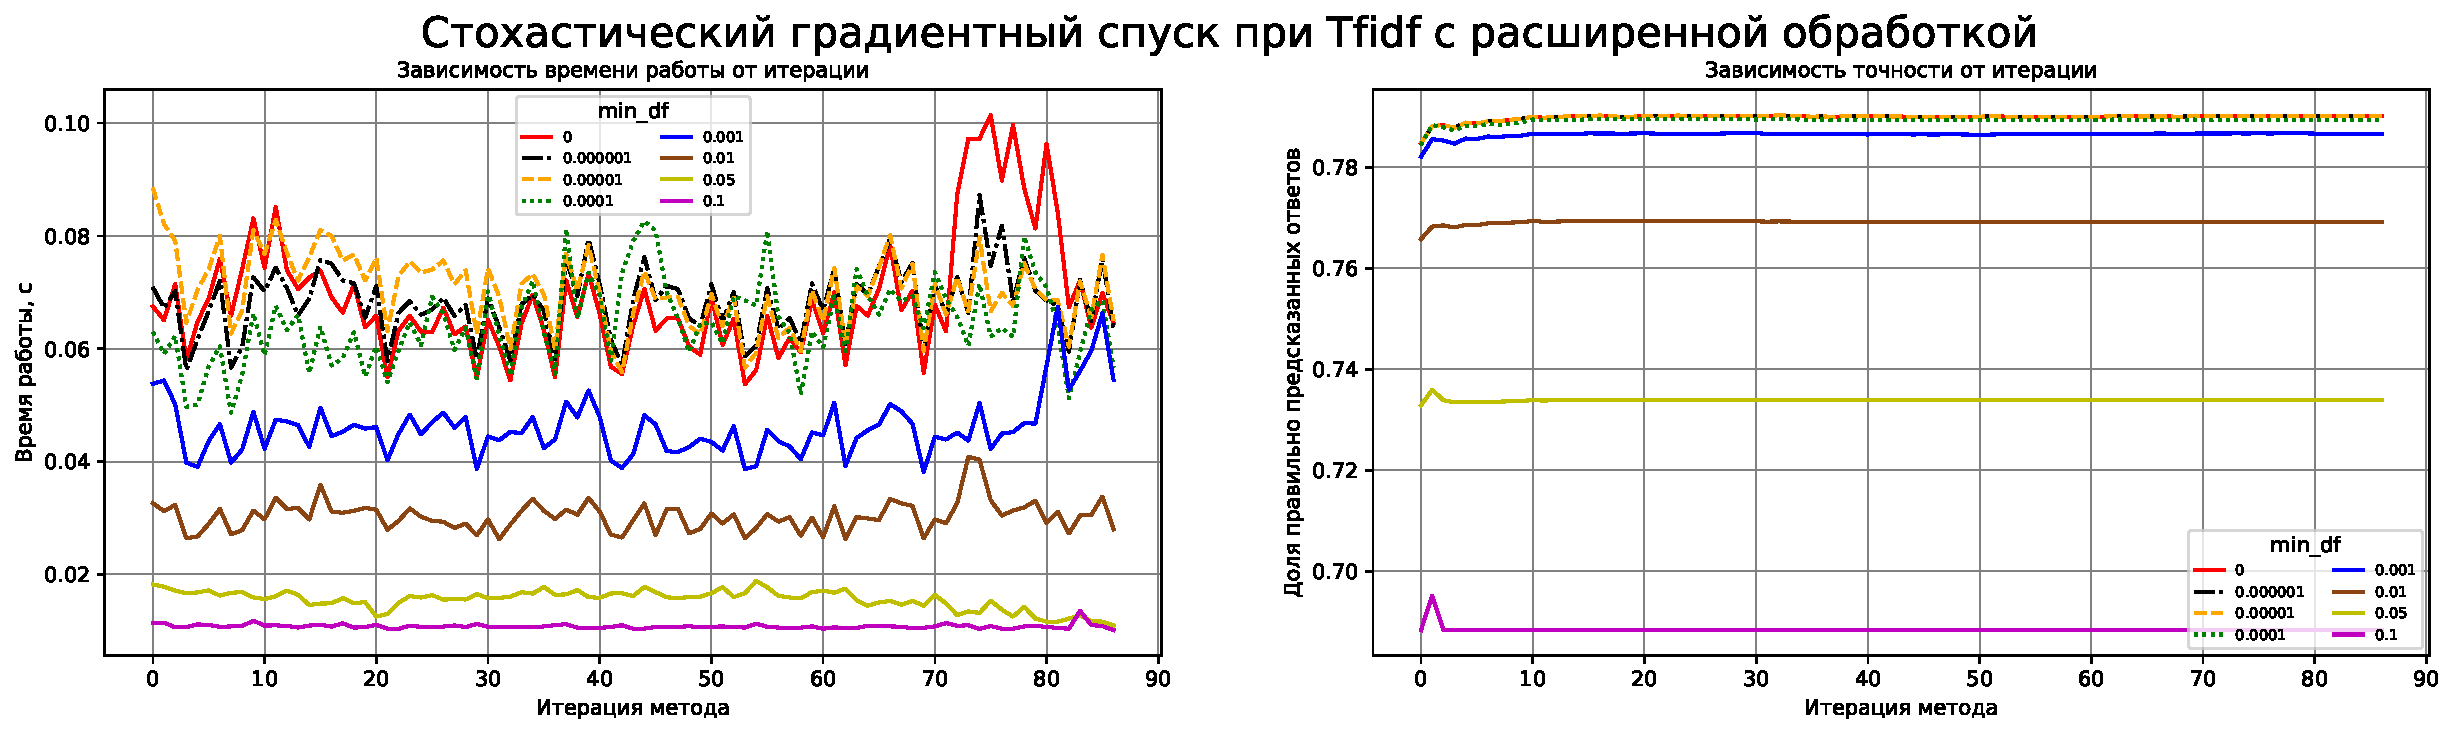
\includegraphics[width=14cm]{TASK2 min_df Tfidf SGD.pdf}
	\caption{Поведение стохастического градиентного спуска при представлении Tf-Idf и изменении параметра min\_df}
	\label{fig:min_df_Tfidf_SGD}
\end{figure}
\begin{figure}[H]
	\centering
	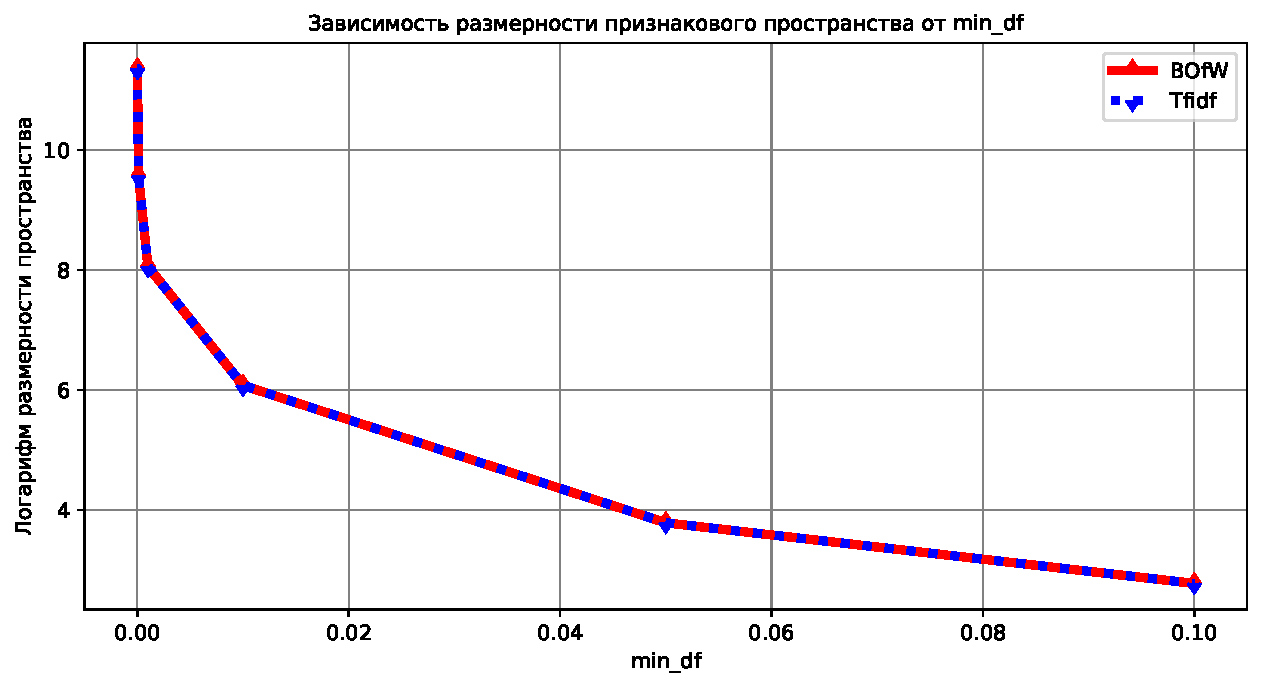
\includegraphics[width=10cm]{TASK2 min_df size.pdf}
	\caption{Размерность признакового пространства при различных min\_df}
	\label{fig:min_df_size}
\end{figure}


  \item Изменение параметра max\_df

Параметр max\_df перебирается по сетке: \{1.0, 0.2, 0.1, 0.05, 0.001, 0.0005, 0.0001, 0.00005\}. При этом значение min\_df изменено на значение по умолчанию. В отличие от случая с изменением параметра min\_df, при уменьшении размерности признакового пространства в данном случае заметно улучшение качества работы модели, кроме последнего значения в сетке (рис. \ref{fig:max_df_BagOfWords_GD}, \ref{fig:max_df_BagOfWords_SGD}, \ref{fig:max_df_Tfidf_GD}, \ref{fig:max_df_Tfidf_SGD}). Таким образом, наибольшую точность дает max\_df=0.0001. Заметим, что при трех максимальных перебранных max\_df (1.0, 0.2, 0.1) точность не изменяется, но это связано с тем, что не меняется размерность признакового пространства (рис. \ref{fig:max_df_size}). При уменьшении размерности признакового пространства (то есть, уменьшении max\_df) время работы программы уменьшается.

\begin{figure}[H]
	\centering
	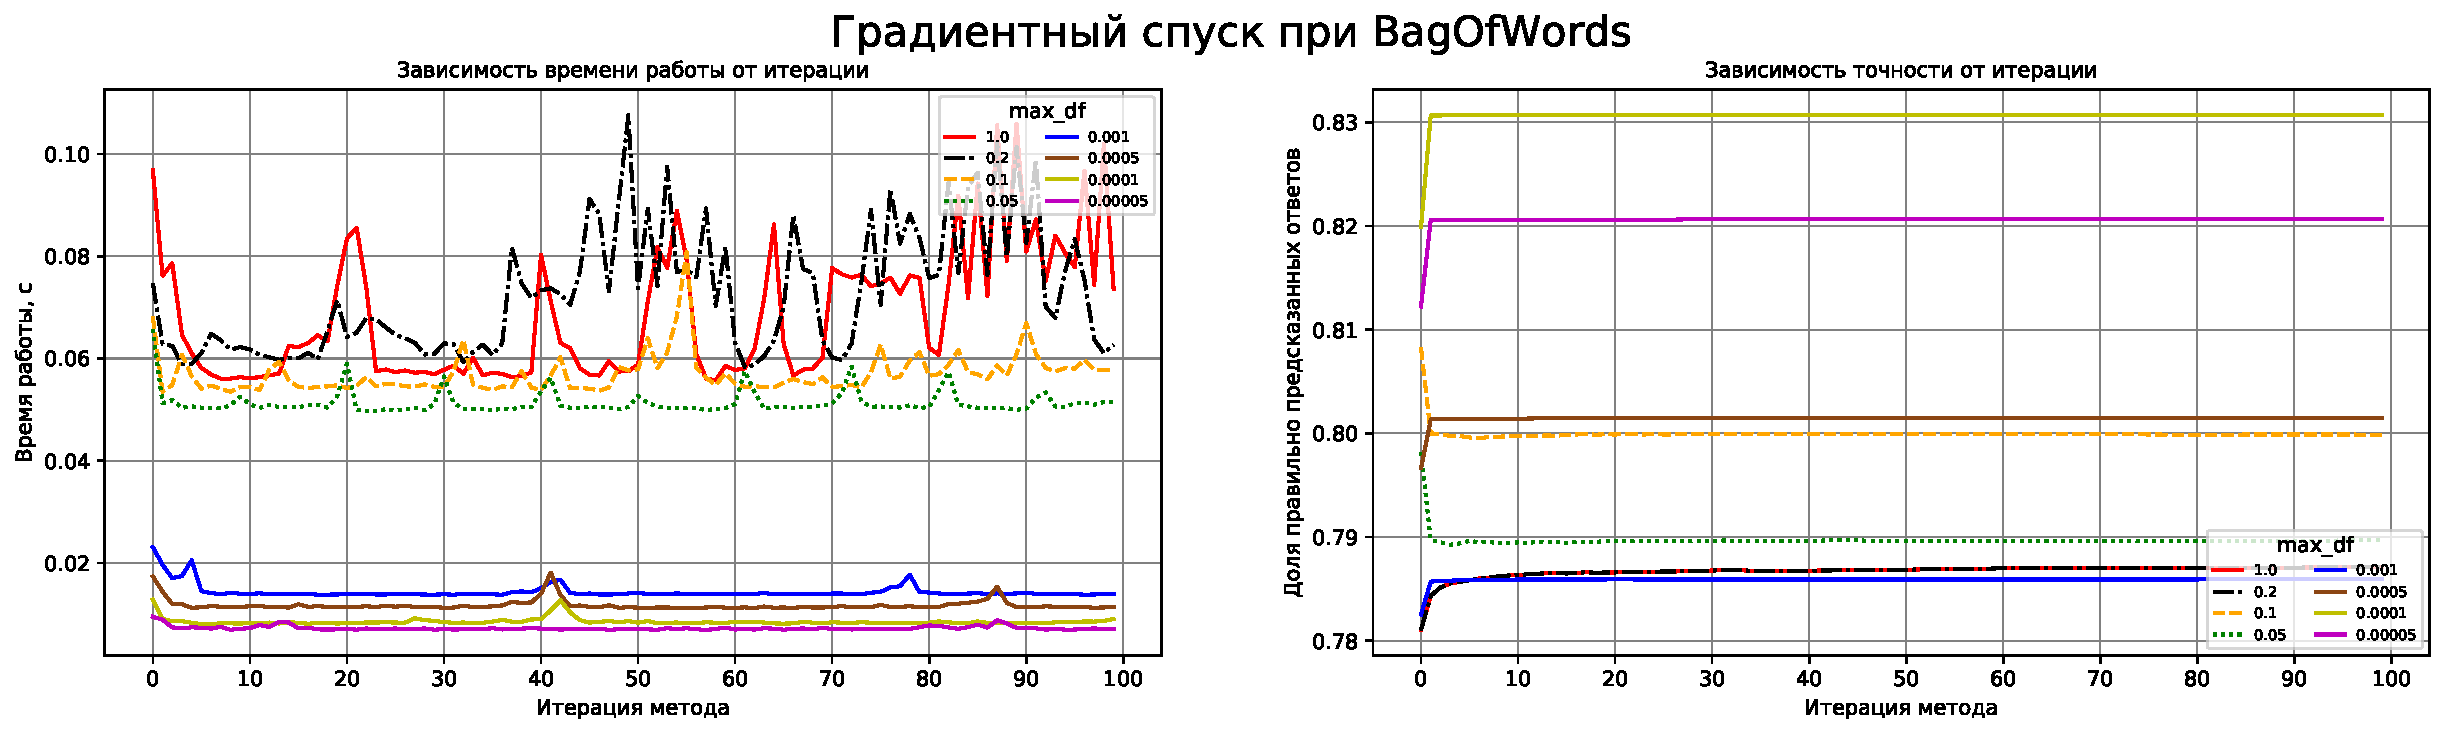
\includegraphics[width=15cm]{TASK2 max_df BagOfWords GD.pdf}
	\caption{Поведение градиентного спуска при представлении Bag Of Words и изменении параметра max\_df}
	\label{fig:max_df_BagOfWords_GD}
\end{figure}
\begin{figure}[H]
	\centering
	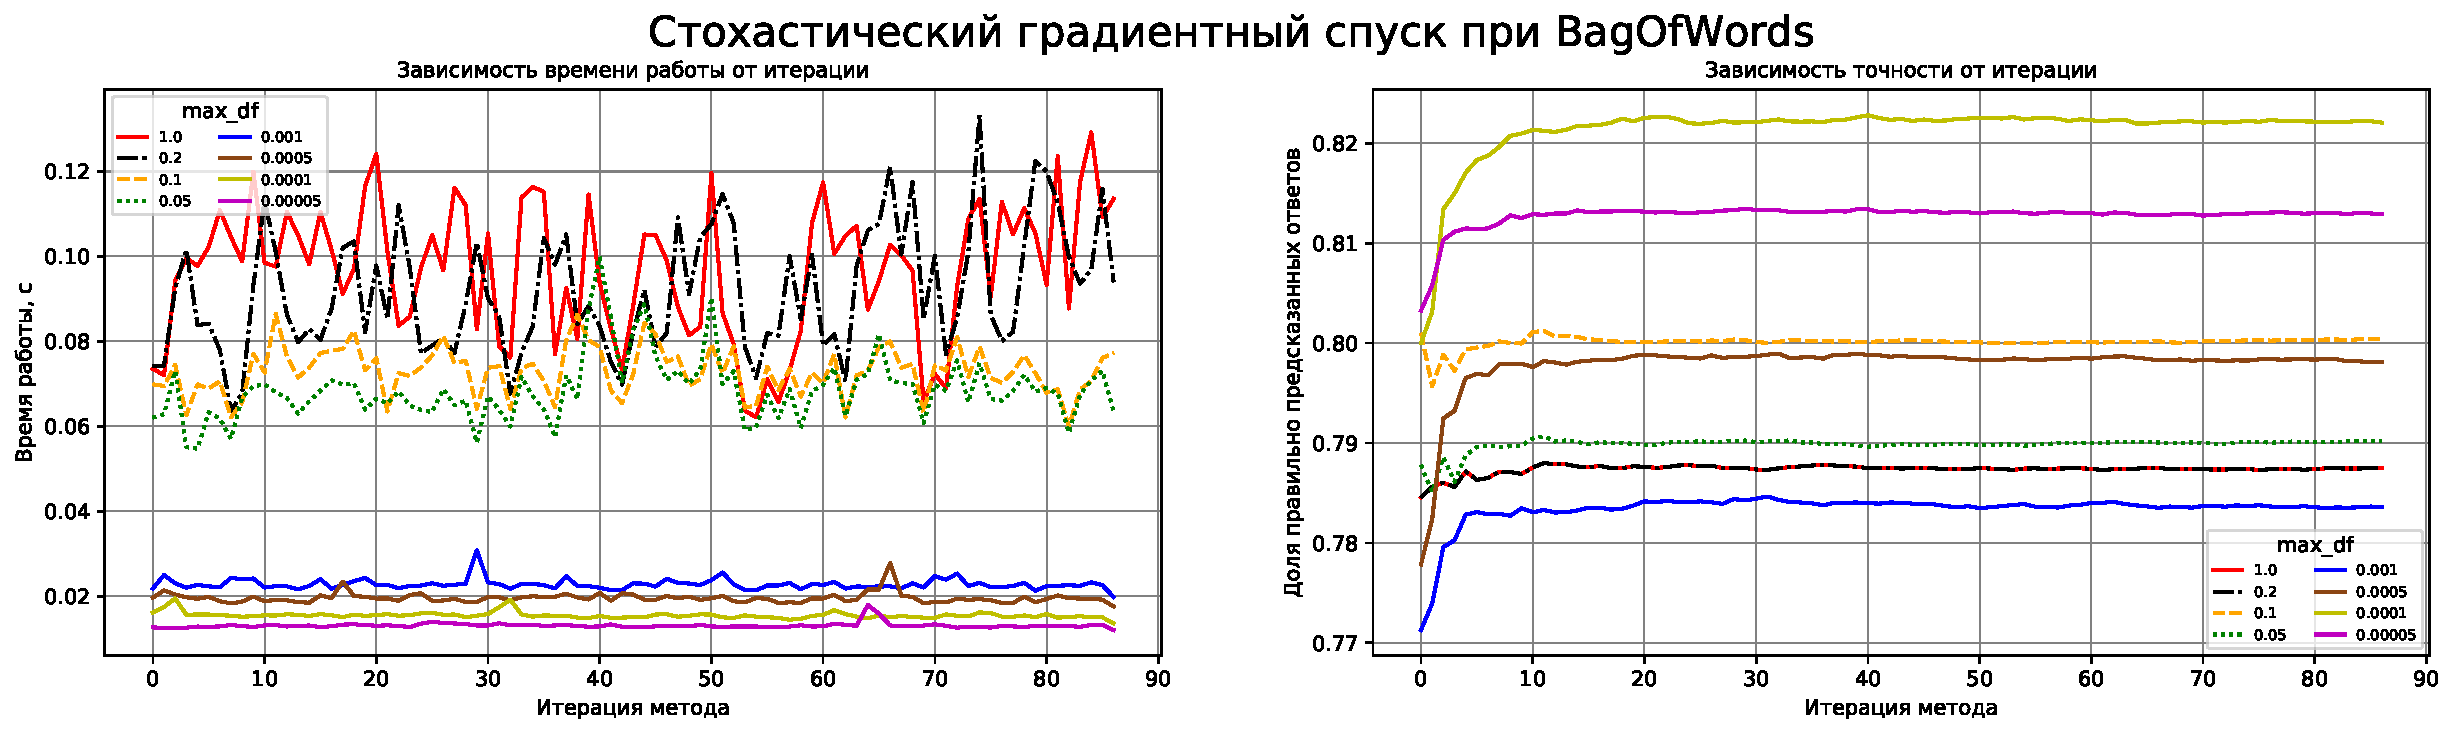
\includegraphics[width=15cm]{TASK2 max_df BagOfWords SGD.pdf}
	\caption{Поведение стохастического градиентного спуска при представлении Bag Of Words и изменении параметра max\_df}
	\label{fig:max_df_BagOfWords_SGD}
\end{figure}
\begin{figure}[H]
	\centering
	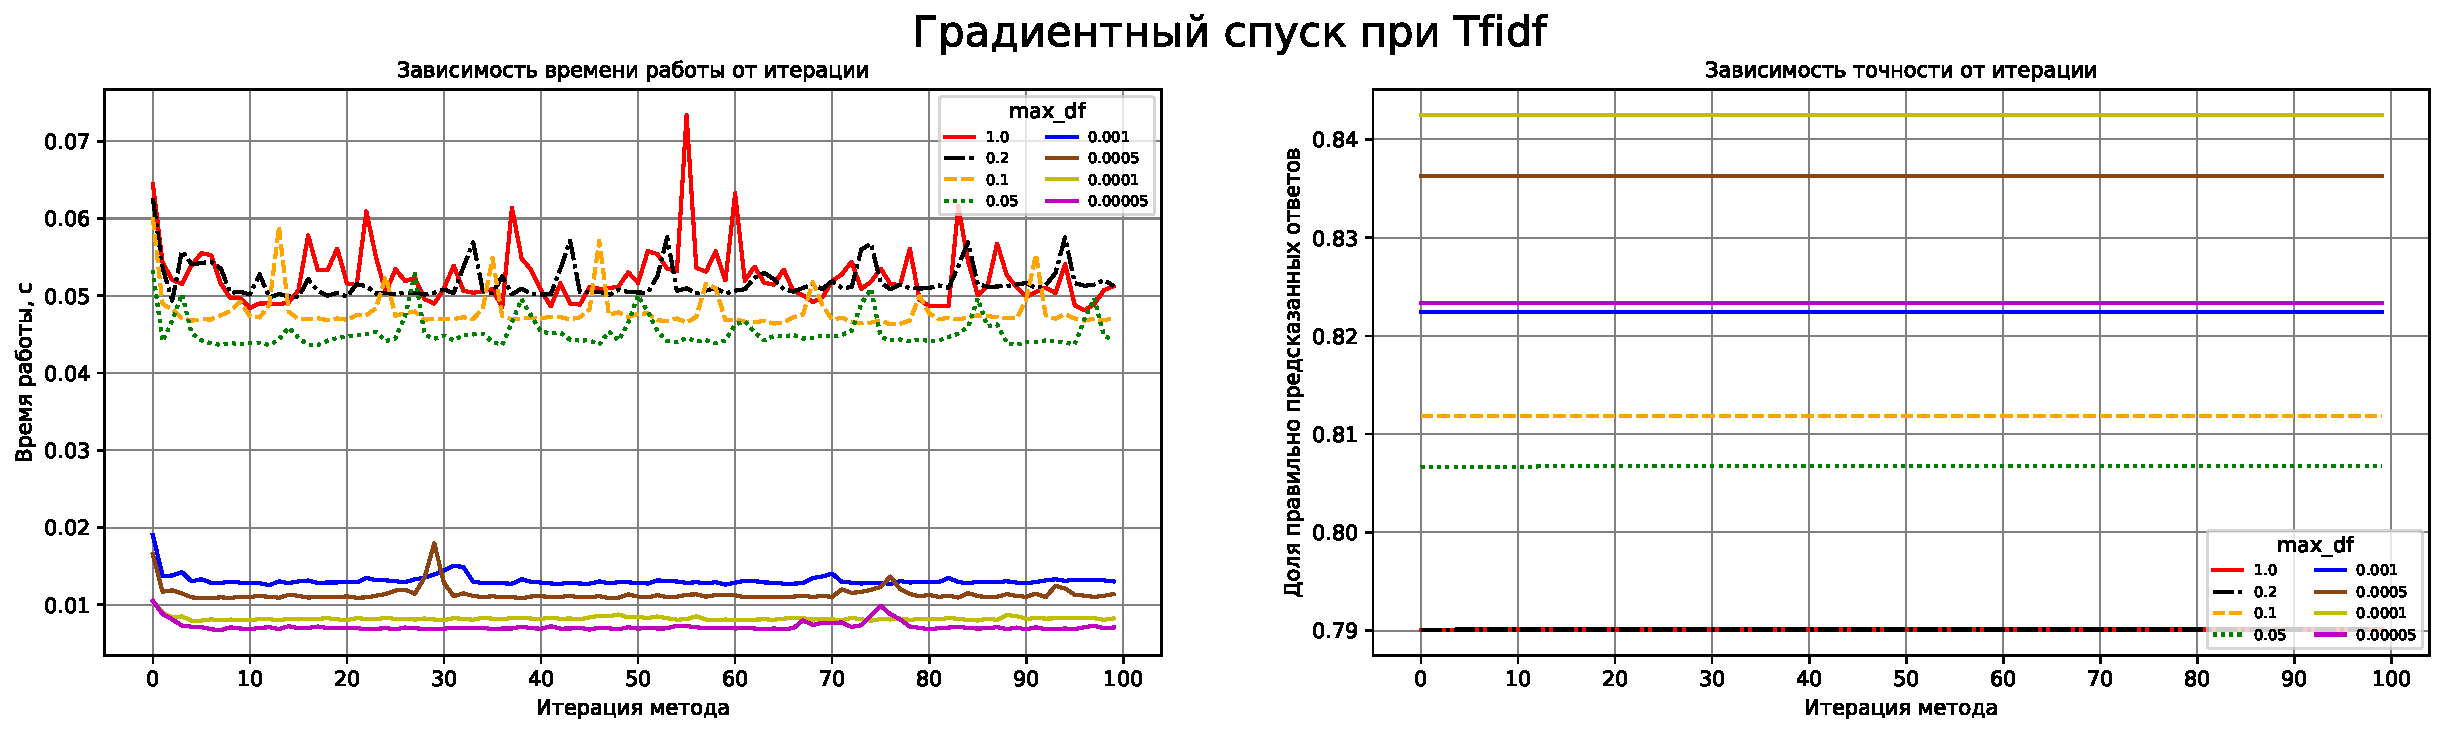
\includegraphics[width=15cm]{TASK2 max_df Tfidf GD.pdf}
	\caption{Поведение градиентного спуска при представлении Tf-Idf и изменении параметра max\_df}
	\label{fig:max_df_Tfidf_GD}
\end{figure}
\begin{figure}[H]
	\centering
	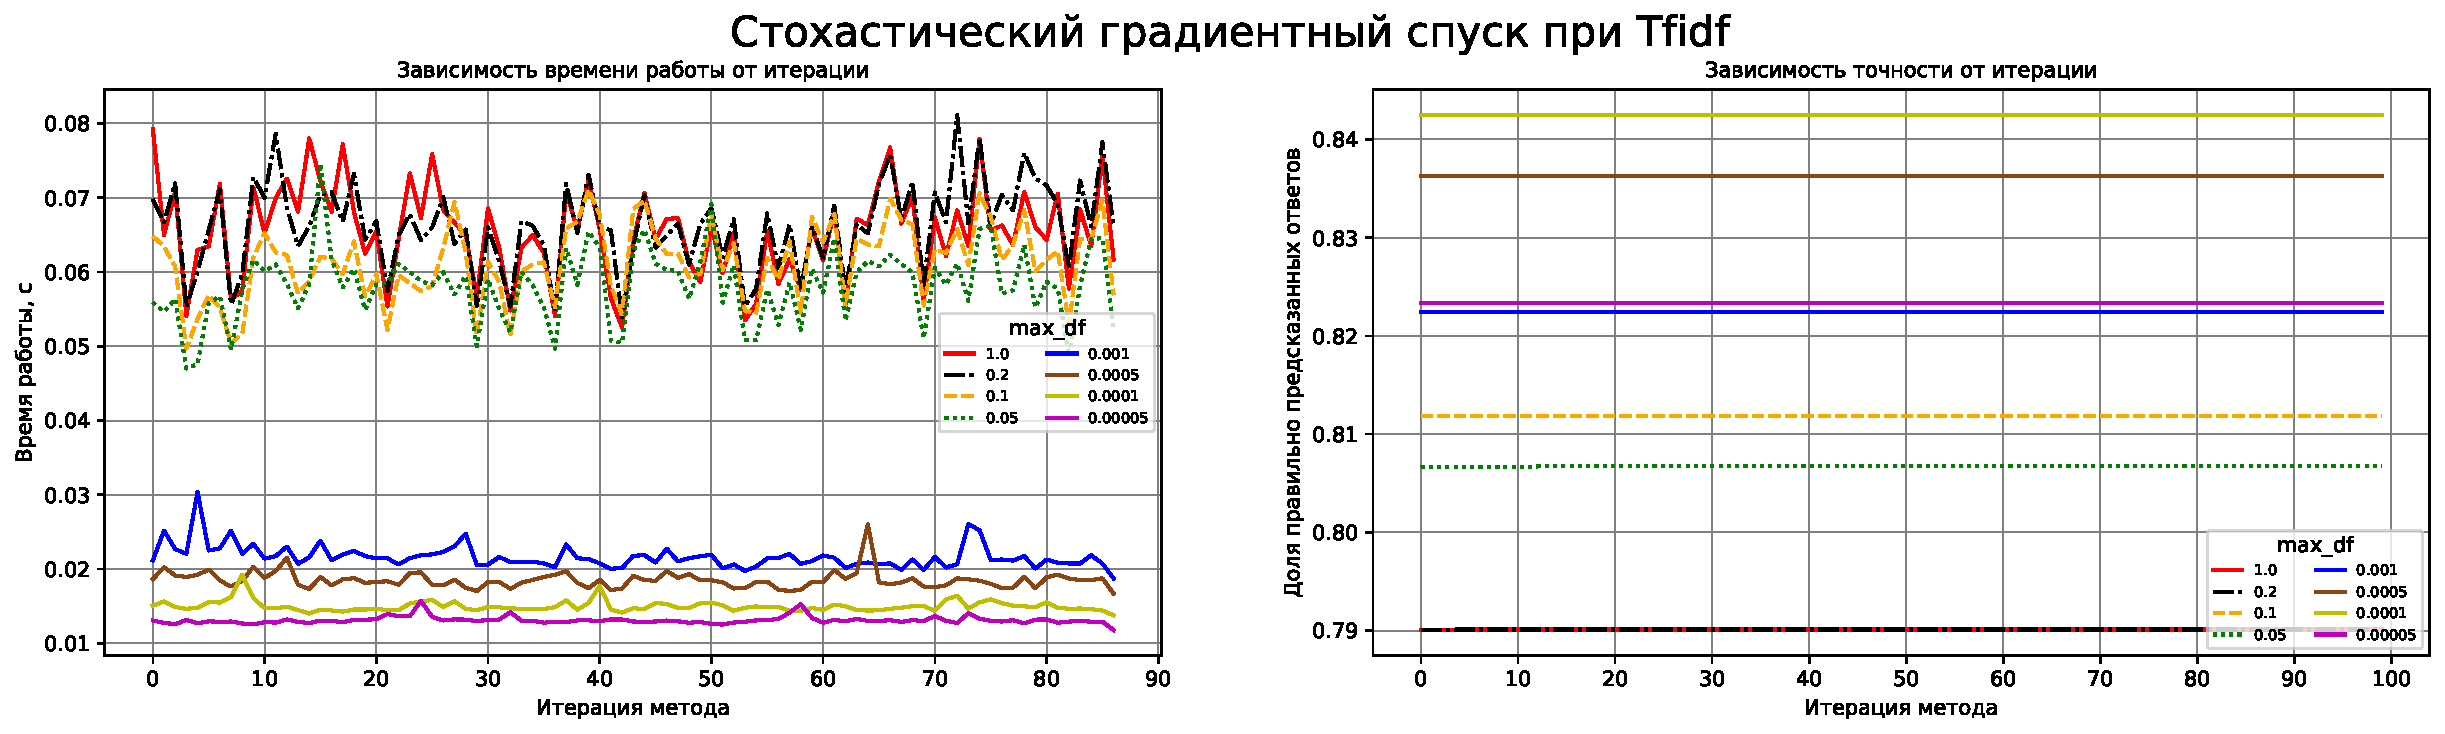
\includegraphics[width=15cm]{TASK2 max_df Tfidf SGD.pdf}
	\caption{Поведение стохастического градиентного спуска при представлении Tf-Idf и изменении параметра max\_df}
	\label{fig:max_df_Tfidf_SGD}
\end{figure}
\begin{figure}[H]
	\centering
	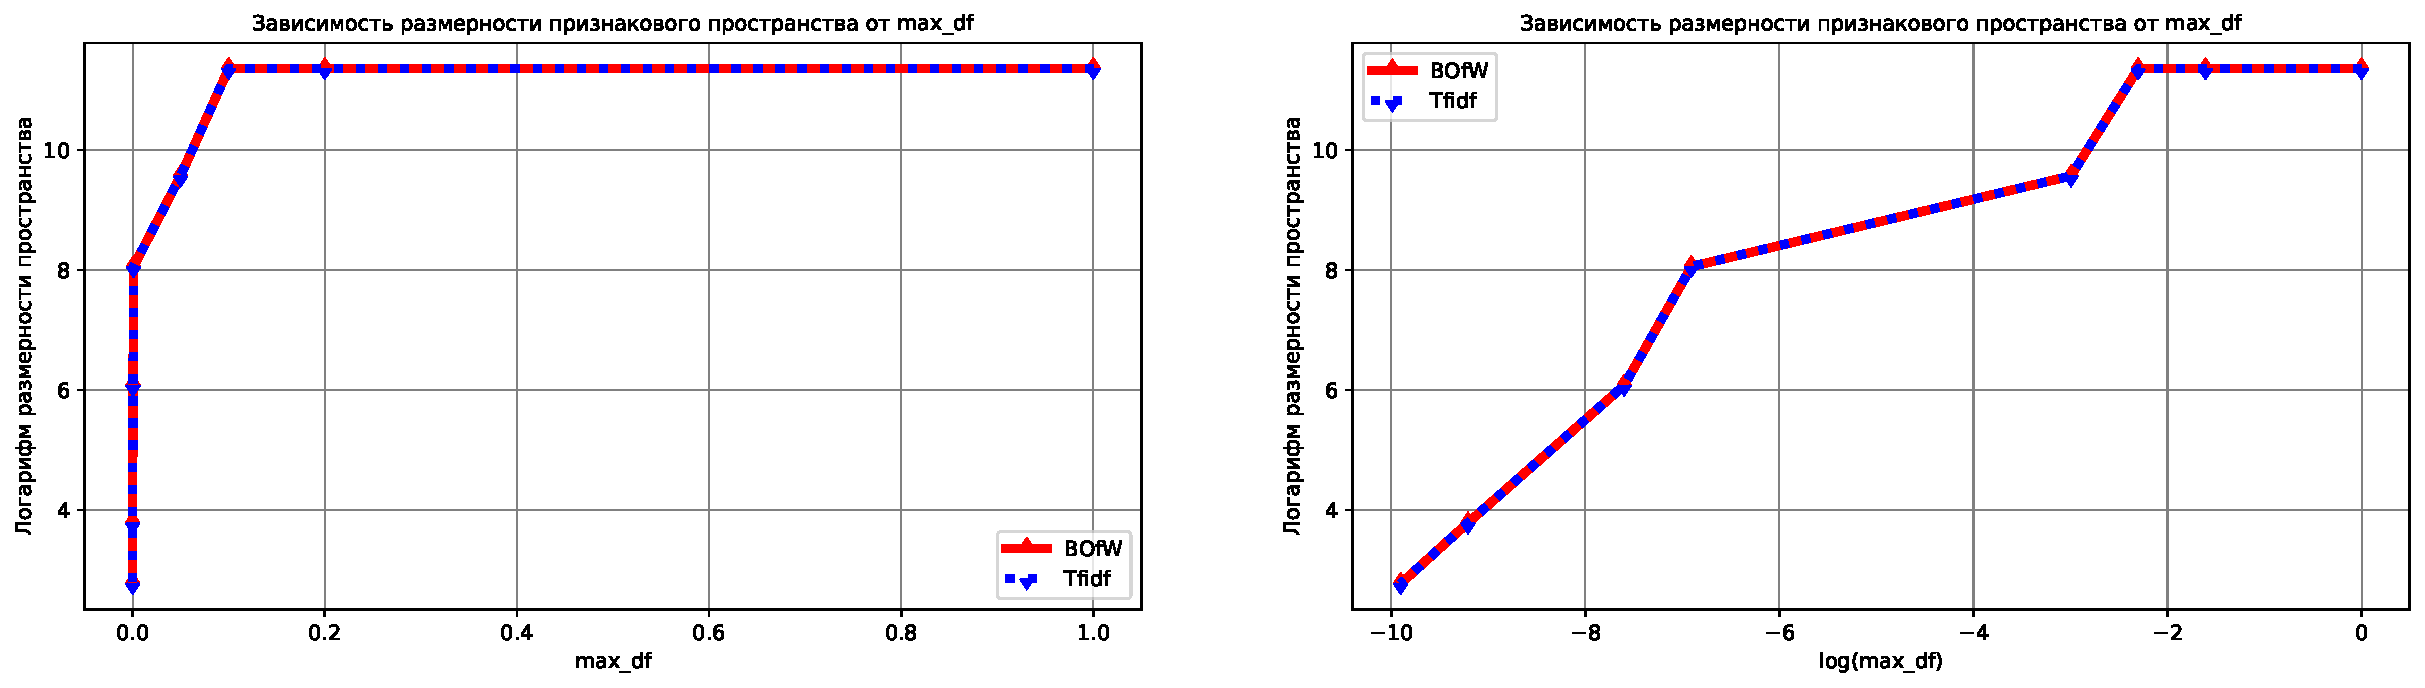
\includegraphics[width=15cm]{TASK2 max_df size.pdf}
	\caption{Размерность признакового пространства при различных max\_df}
	\label{fig:max_df_size}
\end{figure}


\end{itemize}


При уменьшении размерности признакового пространства увеличивается скорость работы алгоритма. При этом параметры min\_df и max\_df конструкторов можно подобрать такими, чтобы точность алгоритма не ухудшилась или даже улучшилась.

\section{Проверка лучшего алгоритма на тестовой выборке}
Параметры, лучше всего показавшие себя на обучающей выборке:

\begin{itemize}
  \item step\_alpha=0.5;
  \item step\_beta=1.1;
   \item Одинаковые веса со значениями 0;
   \item Для стохастического градиентного спуска batch\_size=10000;
   \item Представление выборки в виде Tf-Idf с расширенной обработкой;
   \item min\_df = 0.0001;
   \item max\_df = 0.0001.
\end{itemize}

В таблице \ref{tabl:Textssylki} представлены значения точности, полученные на тестовой выборке при данных параметрах и изменениях параметров min\_df и max\_df. Здесь GD – градиентный спуск, SGD – стохастический градиентный спуск. 

Изменения параметров min\_df и max\_df связаны с тем, что при одновременном применении min\_df = 0.0001 и max\_df = 0.0001 размер выборки уменьшился настолько, что представление тестовой выборки при TfidfVectorizer стало невозможным. Поэтому параметр min\_df был уменьшен до 0.00005. При одновременном применении параметров min\_df и max\_df точность показала достаточно низкий результат (0.6959 и 0.6885 при градиентном и стохастическом градиентном спуске соответственно). Это можно связать с переобучением: при расширенной обработке выборки из нее и так были удалены часто встречающиеся слова. Следующие столбцы таблицы показывают, что низкие значения точности на тестовой выборке связаны именно с применением параметра max\_df со значением не по умолчанию. Также на всякий случай проверено, что min\_df = 0.0001 дает лучший результат, чем min\_df = 0.00005.


\begin{table}[H]
\begin{tabular}{|l|l|l|l|l|l|}
\hline
    & \begin{tabular}[l]{@{}l@{}}max\_df =  0.0001\\  min\_df = 0.0001\end{tabular} & \begin{tabular}[l]{@{}l@{}}max\_df =  0.0001\\  min\_df = 0.00005\end{tabular} & \begin{tabular}[l]{@{}l@{}}max\_df =  0.0001\\  min\_df = 1\end{tabular} & \begin{tabular}[l]{@{}l@{}}max\_df = 1.0\\  min\_df = 0.0001\end{tabular} & \begin{tabular}[l]{@{}l@{}}max\_df = 1.0\\  min\_df = 0.00005\end{tabular} \\ \hline
GD  & – & 0.6959 & 0.6901 & 0.8159 & 0.8153 \\ \hline
SGD & – & 0.6885 & 0.6810 & 0.8138 & 0.8132 \\ \hline
\end{tabular}
\caption{Зависимость точности на тестовой выборке от параметров конструкторов}
\label{tabl:Textssylki}
\end{table}

Ниже представлена матрица ошибок алгоритма на тестовой выборке при градиентном спуске и параметре min\_df = 0.0001 (рис. \ref{fig:conf_mat}). Чаще всего алгоритм допускает ошибку на комментариях, которые на самом являются негативными (True label = -1).

\begin{figure}[H]
	\centering
	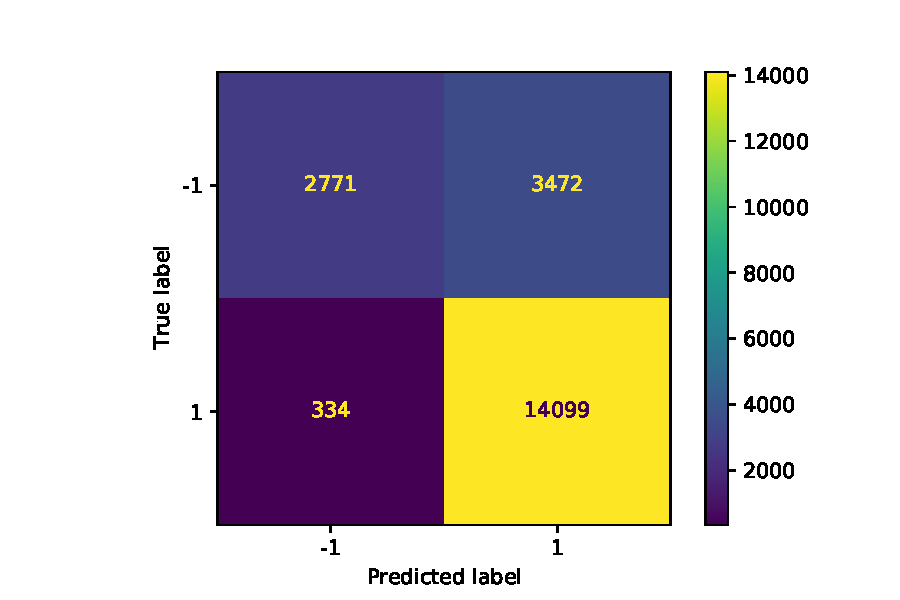
\includegraphics[width=7cm]{conf_mat.pdf}
	\caption{Матрица ошибок при выбранных параметрах}
	\label{fig:conf_mat}
\end{figure}

При просмотре ошибочно определенных комментариях было замечено, что ошибки регулярно встречаются в комментариях, где употребляются слова в переносном значении и поэтому они могут перестать быть негативными или наоборот стать такими (например, слово "hell"{ } использовалось как в негативных комментариях, так и нет – зависело от контекста). Также в обучающей выборке слова, связанные с национальной принадлежностью и религиозными взглядами могли использоваться и в качестве оскорбления, и нет, поэтому на тестовой выборке при классификации таких комментариев были допущены ошибки. В целях сохранения формального стиля отчета тексты комментариев приводиться не будут.

\section{Использование n-грамм}

В данном эксперименте исследуется влияние размера максимальных добавленных n-грамм на качество и скорость работы градиентного спуска при лучших параметрах (обозначенных в предыдущем пункте). 

С увеличением максимально добавленной n-граммы растет точность как на обучающей, так и на тестовой выборке (рис. \ref{fig:n_gram}, \ref{fig:n_gram_test}). При этом точность на тестовой выборке увеличилась на 0.25\%. Однако, добавление n-грамм приводит к увеличению времени. Рост максимальной n-граммы ведет к росту времени. Например, для максимально исследованной n-граммы (15) время выполнения увеличилось в два раза.


\begin{figure}[H]
	\centering
	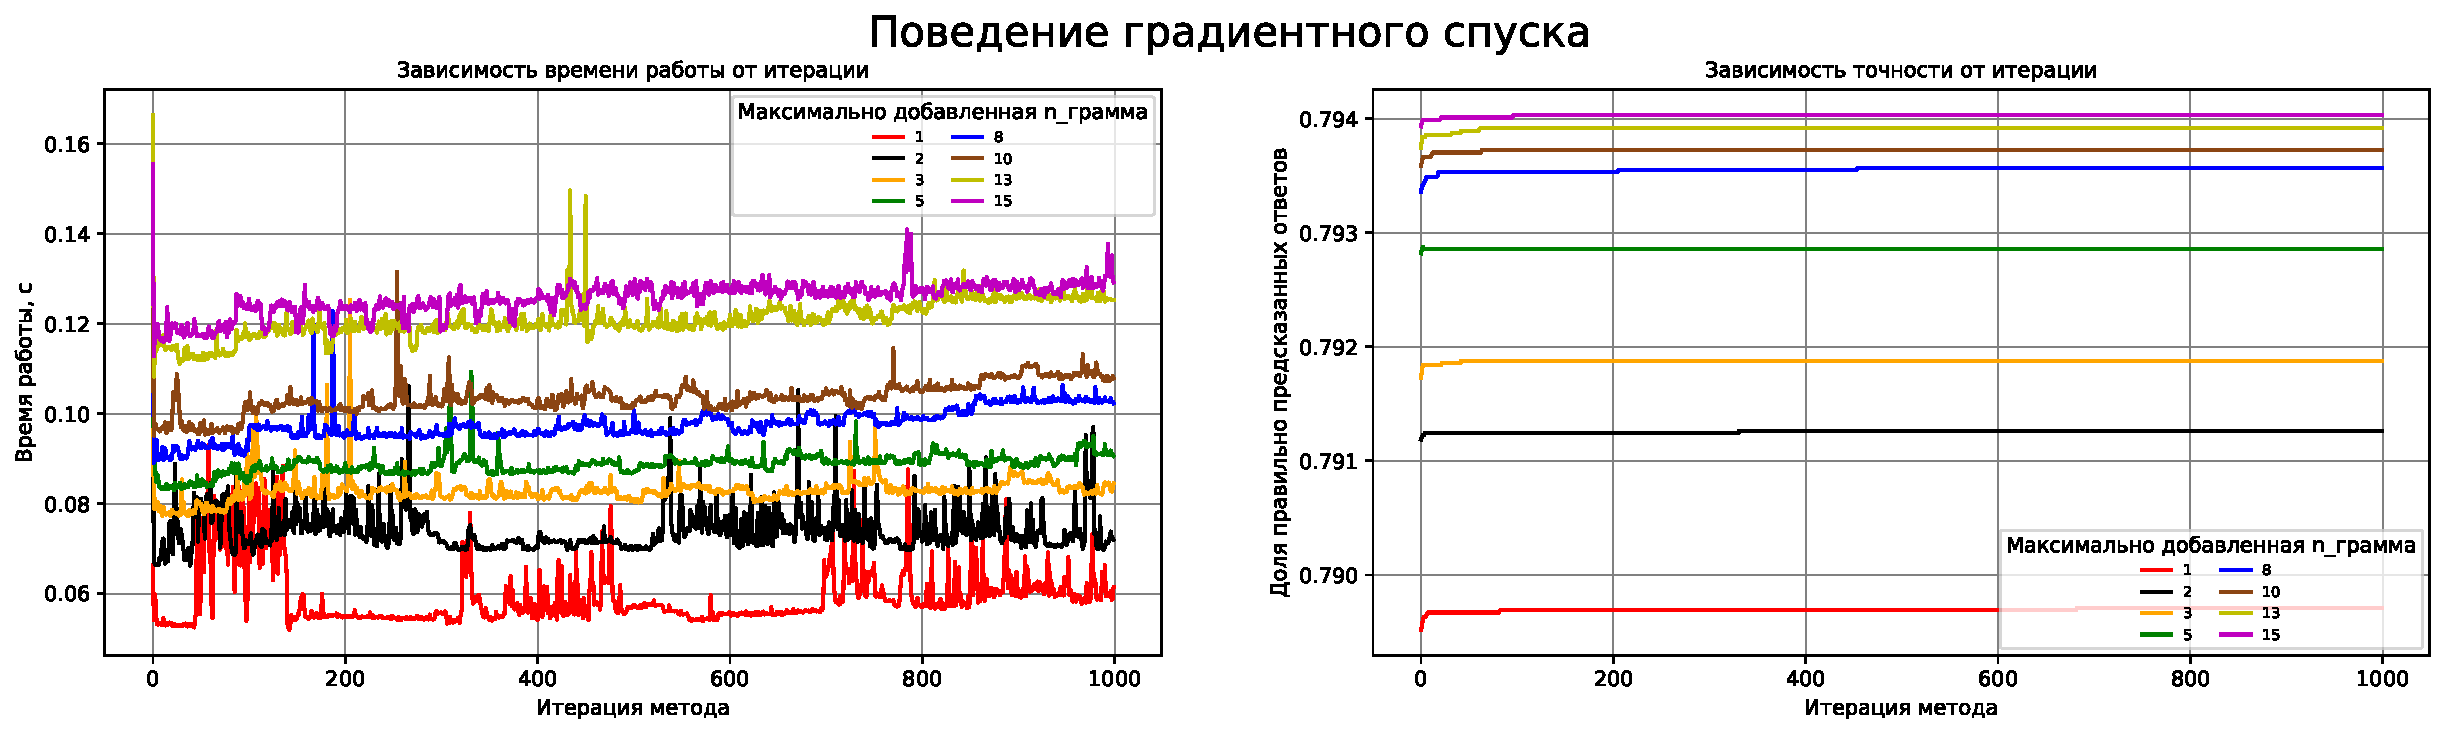
\includegraphics[width=15cm]{TASK2 n_gram.pdf}
	\caption{Влияние максимально добавленной n-граммы на поведение градиентного спуска на обучающей выборке}
	\label{fig:n_gram}
\end{figure}
\begin{figure}[H]
	\centering
	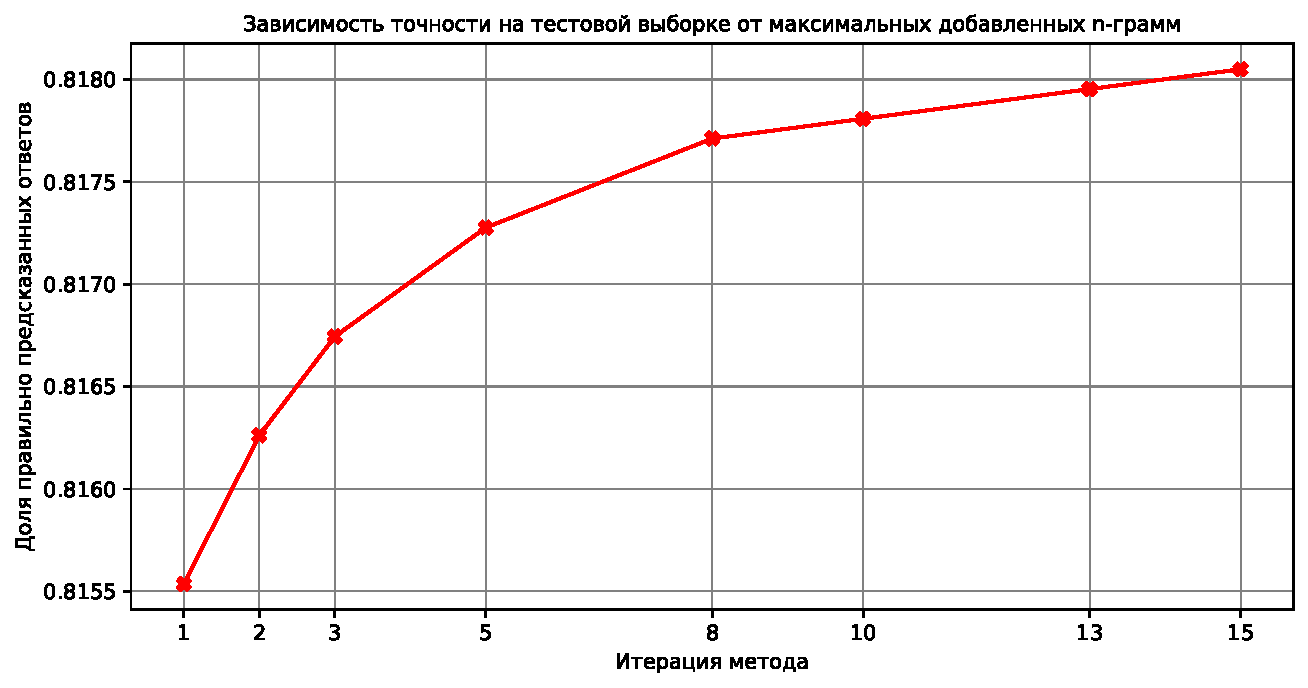
\includegraphics[width=10cm]{TASK2 n_gram test.pdf}
	\caption{Влияние максимально добавленной n-граммы на точность на тестовой выборке}
	\label{fig:n_gram_test}
\end{figure}

\section{Дополнительные улучшения}

Так как негативные комментарии часто пишут с восклицательными знаками, принято решение преобразовать тестовую и обучающую выборку без удаления этих символов. Используется градиентный спуск при параметрах, обозначенных ранее, а также с использованием n-граммы (1, 15). При этом получена точность на тестовой выборке 0.8188, что немного улучшило качество модели.

Далее принято решение удалить восклицательные знаки из обучающей выборки только в не токсичных комментариях. При данной обработке получена точность на тестовой выборке 0.8189.

\section{Выводы}

Изучены методы градиентного и стохастического градиентного спуска в задаче бинарной классификации текстов. Исследована зависимость скорости работы и точности моделей в зависимости от различных параметров. Исследованы два способа представления выборки: Bag of words и Tf-Idf, а также способы уменьшения признакового пространства и их влияние на работу алгоритма. 

\newpage
\addcontentsline{toc}{section}{Список используемой литературы}
\begin{thebibliography}{}
    \bibitem{ss0} \href{http://www.machinelearning.ru/wiki/index.php?title=Стохастический_градиентный_спуск}{ Machinelearning – стохастический градиентный спуск}
    \bibitem{ss1} \href{https://github.com/mmp-practicum-team/mmp_practicum_fall_2022/blob/main/Seminars/08-text-processing-and-logreg/linear_classifier.ipynb}{Ноутбук с семинара}
    \bibitem{ss2} \href{https://overcoder.net/q/169195/понимание-mindf-и-maxdf-в-scikit-countvectorizer}{Overcoder – про min\_df и max\_df}
    \bibitem{ss3} \href{https://www.studocu.com/ru/document/mgu-im-lomonosova/cybersecurity/linear-regression-and-gradient-optimization/20403639}{Найдено абсолютно случайно}
    
\end{thebibliography}

\end{document}